% Options for packages loaded elsewhere
\PassOptionsToPackage{unicode}{hyperref}
\PassOptionsToPackage{hyphens}{url}
%
\documentclass[
]{article}
\usepackage{amsmath,amssymb}
\usepackage{iftex}
\ifPDFTeX
  \usepackage[T1]{fontenc}
  \usepackage[utf8]{inputenc}
  \usepackage{textcomp} % provide euro and other symbols
\else % if luatex or xetex
  \usepackage{unicode-math} % this also loads fontspec
  \defaultfontfeatures{Scale=MatchLowercase}
  \defaultfontfeatures[\rmfamily]{Ligatures=TeX,Scale=1}
\fi
\usepackage{lmodern}
\ifPDFTeX\else
  % xetex/luatex font selection
\fi
% Use upquote if available, for straight quotes in verbatim environments
\IfFileExists{upquote.sty}{\usepackage{upquote}}{}
\IfFileExists{microtype.sty}{% use microtype if available
  \usepackage[]{microtype}
  \UseMicrotypeSet[protrusion]{basicmath} % disable protrusion for tt fonts
}{}
\makeatletter
\@ifundefined{KOMAClassName}{% if non-KOMA class
  \IfFileExists{parskip.sty}{%
    \usepackage{parskip}
  }{% else
    \setlength{\parindent}{0pt}
    \setlength{\parskip}{6pt plus 2pt minus 1pt}}
}{% if KOMA class
  \KOMAoptions{parskip=half}}
\makeatother
\usepackage{xcolor}
\usepackage[margin=1in]{geometry}
\usepackage{color}
\usepackage{fancyvrb}
\newcommand{\VerbBar}{|}
\newcommand{\VERB}{\Verb[commandchars=\\\{\}]}
\DefineVerbatimEnvironment{Highlighting}{Verbatim}{commandchars=\\\{\}}
% Add ',fontsize=\small' for more characters per line
\usepackage{framed}
\definecolor{shadecolor}{RGB}{248,248,248}
\newenvironment{Shaded}{\begin{snugshade}}{\end{snugshade}}
\newcommand{\AlertTok}[1]{\textcolor[rgb]{0.94,0.16,0.16}{#1}}
\newcommand{\AnnotationTok}[1]{\textcolor[rgb]{0.56,0.35,0.01}{\textbf{\textit{#1}}}}
\newcommand{\AttributeTok}[1]{\textcolor[rgb]{0.13,0.29,0.53}{#1}}
\newcommand{\BaseNTok}[1]{\textcolor[rgb]{0.00,0.00,0.81}{#1}}
\newcommand{\BuiltInTok}[1]{#1}
\newcommand{\CharTok}[1]{\textcolor[rgb]{0.31,0.60,0.02}{#1}}
\newcommand{\CommentTok}[1]{\textcolor[rgb]{0.56,0.35,0.01}{\textit{#1}}}
\newcommand{\CommentVarTok}[1]{\textcolor[rgb]{0.56,0.35,0.01}{\textbf{\textit{#1}}}}
\newcommand{\ConstantTok}[1]{\textcolor[rgb]{0.56,0.35,0.01}{#1}}
\newcommand{\ControlFlowTok}[1]{\textcolor[rgb]{0.13,0.29,0.53}{\textbf{#1}}}
\newcommand{\DataTypeTok}[1]{\textcolor[rgb]{0.13,0.29,0.53}{#1}}
\newcommand{\DecValTok}[1]{\textcolor[rgb]{0.00,0.00,0.81}{#1}}
\newcommand{\DocumentationTok}[1]{\textcolor[rgb]{0.56,0.35,0.01}{\textbf{\textit{#1}}}}
\newcommand{\ErrorTok}[1]{\textcolor[rgb]{0.64,0.00,0.00}{\textbf{#1}}}
\newcommand{\ExtensionTok}[1]{#1}
\newcommand{\FloatTok}[1]{\textcolor[rgb]{0.00,0.00,0.81}{#1}}
\newcommand{\FunctionTok}[1]{\textcolor[rgb]{0.13,0.29,0.53}{\textbf{#1}}}
\newcommand{\ImportTok}[1]{#1}
\newcommand{\InformationTok}[1]{\textcolor[rgb]{0.56,0.35,0.01}{\textbf{\textit{#1}}}}
\newcommand{\KeywordTok}[1]{\textcolor[rgb]{0.13,0.29,0.53}{\textbf{#1}}}
\newcommand{\NormalTok}[1]{#1}
\newcommand{\OperatorTok}[1]{\textcolor[rgb]{0.81,0.36,0.00}{\textbf{#1}}}
\newcommand{\OtherTok}[1]{\textcolor[rgb]{0.56,0.35,0.01}{#1}}
\newcommand{\PreprocessorTok}[1]{\textcolor[rgb]{0.56,0.35,0.01}{\textit{#1}}}
\newcommand{\RegionMarkerTok}[1]{#1}
\newcommand{\SpecialCharTok}[1]{\textcolor[rgb]{0.81,0.36,0.00}{\textbf{#1}}}
\newcommand{\SpecialStringTok}[1]{\textcolor[rgb]{0.31,0.60,0.02}{#1}}
\newcommand{\StringTok}[1]{\textcolor[rgb]{0.31,0.60,0.02}{#1}}
\newcommand{\VariableTok}[1]{\textcolor[rgb]{0.00,0.00,0.00}{#1}}
\newcommand{\VerbatimStringTok}[1]{\textcolor[rgb]{0.31,0.60,0.02}{#1}}
\newcommand{\WarningTok}[1]{\textcolor[rgb]{0.56,0.35,0.01}{\textbf{\textit{#1}}}}
\usepackage{longtable,booktabs,array}
\usepackage{calc} % for calculating minipage widths
% Correct order of tables after \paragraph or \subparagraph
\usepackage{etoolbox}
\makeatletter
\patchcmd\longtable{\par}{\if@noskipsec\mbox{}\fi\par}{}{}
\makeatother
% Allow footnotes in longtable head/foot
\IfFileExists{footnotehyper.sty}{\usepackage{footnotehyper}}{\usepackage{footnote}}
\makesavenoteenv{longtable}
\usepackage{graphicx}
\makeatletter
\def\maxwidth{\ifdim\Gin@nat@width>\linewidth\linewidth\else\Gin@nat@width\fi}
\def\maxheight{\ifdim\Gin@nat@height>\textheight\textheight\else\Gin@nat@height\fi}
\makeatother
% Scale images if necessary, so that they will not overflow the page
% margins by default, and it is still possible to overwrite the defaults
% using explicit options in \includegraphics[width, height, ...]{}
\setkeys{Gin}{width=\maxwidth,height=\maxheight,keepaspectratio}
% Set default figure placement to htbp
\makeatletter
\def\fps@figure{htbp}
\makeatother
\setlength{\emergencystretch}{3em} % prevent overfull lines
\providecommand{\tightlist}{%
  \setlength{\itemsep}{0pt}\setlength{\parskip}{0pt}}
\setcounter{secnumdepth}{-\maxdimen} % remove section numbering
\ifLuaTeX
  \usepackage{selnolig}  % disable illegal ligatures
\fi
\IfFileExists{bookmark.sty}{\usepackage{bookmark}}{\usepackage{hyperref}}
\IfFileExists{xurl.sty}{\usepackage{xurl}}{} % add URL line breaks if available
\urlstyle{same}
\hypersetup{
  pdftitle={Demand for health care in Australia},
  pdfauthor={Group O: Buscema Andrea, Cusma Fait Omar, Derin Tanja, Špringer Christian, Zivanovic Uros},
  hidelinks,
  pdfcreator={LaTeX via pandoc}}

\title{Demand for health care in Australia}
\usepackage{etoolbox}
\makeatletter
\providecommand{\subtitle}[1]{% add subtitle to \maketitle
  \apptocmd{\@title}{\par {\large #1 \par}}{}{}
}
\makeatother
\subtitle{Final Project for Statistical Methods}
\author{Group O: Buscema Andrea, Cusma Fait Omar, Derin Tanja, Špringer
Christian, Zivanovic Uros}
\date{2024-03-01}

\begin{document}
\maketitle

{
\setcounter{tocdepth}{3}
\tableofcontents
}
\section{ABSTRACT}\label{abstract}

In this final project for the course ``344SM - Statistical Methods'' we
will analyze the dataset based on the Australian health survey from 1977
to 1978. The dataset contains information of 5190 individuals and 19
variables, including the response variable `doctorco', which is the
number of consulations with a doctor or specialist in the past 2 weeks.

For the purpose of this project, after the initial data exploration
analysis, including the data cleaning and the data visualization, we
will focus on the prediction of the number of consulations with a doctor
or specialist in the past 2 weeks. We will use:

\begin{itemize}
\tightlist
\item
  Negative Binomial regression
\item
  Zero-inflated Poisson regression
\item
  Zero-inflated Negative Binomial regression
\item
  Hurdle Poisson regression
\item
  Hurdle Negative Binomial regression
\item
  Logistic regression
\item
  Random Forest
\item
  Naive Bayes
\item
  Neural Networks
\item
  K-Nearest Neighbors
\end{itemize}

The whole project was implemented with two programming languages, R and
Python, thereby harnessing the specialized capabilities of each to
create a robust, efficient, and versatile analytical workflow. This
dual-language approach facilitated the leveraging of R's advanced
statistical analysis and visualization tools alongside Python's superior
data manipulation, machine learning, and integration capabilities. As a
result, the project benefited from the rich and diverse libraries of
both ecosystems, ensuring that each stage of the project, from data
cleaning to complex statistical modeling and even deployment, was
handled with the most effective tools available. This method not only
enhanced the overall quality and depth of the analysis but also fostered
a flexible and innovative environment for tackling the multifaceted
challenges of the project.

\#\#Dataset

The dataset contains information divided into these 19 variables:

\begin{itemize}
\tightlist
\item
  \textbf{Categorical (Binary) variables:}

  \begin{itemize}
  \tightlist
  \item
    `sex': gender of the individual (1 if female, 0 if male);
  \item
    `levyplus': 1 if covered by private health insurance fund for
    private patient in public hospital (with doctor of choice), 0
    otherwise;
  \item
    `freepoor': 1 if covered by government because of low income, recent
    immigrant, unemployed, 0 otherwise;
  \item
    `freepera': 1 if covered by government because of old-age or
    disability pension, or because invalid veteran or family of deceased
    veteran, 0 otherwise;
  \item
    `chcond1': 1 if chronic condition(s) but not limited in activity, 0
    otherwise;
  \item
    `chcond2': 1 if chronic condition(s) and limited in activity, 0
    otherwise;
  \end{itemize}
\item
  \textbf{Categorical (Ordinal) variables:}

  \begin{itemize}
  \tightlist
  \item
    `age': age in years divided by 100 (measured as mid-point of the age
    groups from 15-19 years to 65-69 years with the last group being 70
    years and over treated as 72);
  \item
    `agesq': `age' squared;
  \item
    `income': Annual income in Australian dollars divided by 1000
    (measured as mid-point of coded ranges Nil, \textless{} 200,
    200-1000, 1001-, 2001-, 3001-, 4001-, 5001-, 6001-, 7001-,
    8001-10000, 10001-12000, 12001-14000, with 14001- treated as 15000);
  \item
    `hscore': General health questionnaire score using Goldberg's
    method. High score indicates bad health;
  \end{itemize}
\item
  \textbf{Discrete variables:}

  \begin{itemize}
  \tightlist
  \item
    `illness': Number of illnesses in the past 2 weeks with 5 or more
    coded as 5;
  \item
    `actdays': Number of days in the past 2 weeks with activity
    limitation due to illness or injury;
  \item
    `doctorco': (Response variable) Number of consultations with a
    doctor or specialist in the past 2 weeks;
  \item
    `nondocco': Number of consultations with non-doctor health
    professional (chemist, optician, physiotherapist, social worker,
    district community nurse, chiropodist or chiropractor, etc.) in the
    past 2 weeks;
  \item
    `hospadmi': Number of admissions to a hospital, psychiatric
    hospital, nursing or convalescent home in the past 12 months (up to
    5 or more admissions which is coded as 5);
  \item
    `hospdays': Number of nights in a hospital, etc. during most recent
    admission: taken, where appropriate, s the mid-point of the
    intervals 1, 2, 3, 4, 5, 6, 7, 8-14, 15-30, 31-60, 61-79 with 80 or
    more admissions coded as 80. If no admission in past 12 months the
    coded as 0;
  \item
    `medicine': Total number of prescribed and nonprescribed medications
    used in past 2 weeks;
  \item
    `prescrib': Number of prescribed medications used in past 2 weeks;
  \item
    `nonpresc': Number of nonprescribed medications used in past 2
    weeks;
  \end{itemize}
\end{itemize}

\textbf{Considerations and before starting the analysis - Levy in
Australia health care in 70-80s}

Health care in Australia during 1977-1978 was is a transitional phase,
with major focus on a universal health insurance system called Medibank.
The Medibank scheme was introduced by the Whitlam Government in 1975
through the Health Insurance Act 1973. The scheme was intended to
provide universal health insurance to all Australians and to provide
free treatment in public hospitals. The scheme was to be funded by a
2.5\% levy on taxable incomes, an additional levy on high-income
earners, as well as government funding. The Medibank scheme was later
abolished by the Fraser Government in 1981, and replaced by a
government-subsidised private insurance scheme, called Medibank Private,
which exists to this day. The dataset we are using is from the period
when the Medibank scheme was in place, and it is interesting to see how
the health care system was functioning at that time.

The Australian health care system has a federal structure, with
responsibilities split between federal and state/territory governments.
The federal government was primarly responsible for funding and policy,
while the state/territory governments were responsible for the delivery
of health care services. The cost of running Medibank was a significant
concerns for the government during this period. There were debates aboyt
whether Medibank provided truly equitable access for all Australians and
concerns about longer waiting times in the public system.

\section{Explanatory Data Analysis}\label{explanatory-data-analysis}

Despite the oldness of the dataset, it doesn't contain any missing value
and the data is clean. Firstly, we will explore the dataset by looking
at the distribution of the response variable `doctorco' and the
distribution of the other variables. Then, we will look at the
correlation between the variables and the response variable.

For this analysis, we excluded `agesq' (age squared) from data frame
while maintaining `age' in this analysis to simplify models and make it
more interpretable, and avoid potential issues like redundancy and
multicollinearity, without significantly compromising the accuracy of
analysis.

\begin{verbatim}
## Rows: 5190 Columns: 20
## -- Column specification --------------------------------------------------------
## Delimiter: ","
## dbl (20): sex, age, agesq, income, levyplus, freepoor, freepera, illness, ac...
## 
## i Use `spec()` to retrieve the full column specification for this data.
## i Specify the column types or set `show_col_types = FALSE` to quiet this message.
\end{verbatim}

\subsection{Dataset Analysis}\label{dataset-analysis}

We start to analyse response variable and independent variables.

\subsubsection{Response variable:
`doctorco'}\label{response-variable-doctorco}

\begin{Shaded}
\begin{Highlighting}[]
\FunctionTok{describe}\NormalTok{(df}\SpecialCharTok{$}\NormalTok{doctorco)}
\end{Highlighting}
\end{Shaded}

\begin{verbatim}
## df$doctorco 
##        n  missing distinct     Info     Mean      Gmd      .05      .10 
##     5190        0       10    0.489   0.3017   0.5154        0        0 
##      .25      .50      .75      .90      .95 
##        0        0        0        1        2 
##                                                                       
## Value          0     1     2     3     4     5     6     7     8     9
## Frequency   4141   782   174    30    24     9    12    12     5     1
## Proportion 0.798 0.151 0.034 0.006 0.005 0.002 0.002 0.002 0.001 0.000
## 
## For the frequency table, variable is rounded to the nearest 0
\end{verbatim}

\begin{Shaded}
\begin{Highlighting}[]
\NormalTok{df }\SpecialCharTok{\%\textgreater{}\%}
  \FunctionTok{ggplot}\NormalTok{(}\FunctionTok{aes}\NormalTok{(}\AttributeTok{x =}\NormalTok{ doctorco)) }\SpecialCharTok{+}
  \FunctionTok{geom\_histogram}\NormalTok{(}\FunctionTok{aes}\NormalTok{(}\AttributeTok{y =} \FunctionTok{after\_stat}\NormalTok{(density)), }\AttributeTok{color =} \StringTok{"black"}\NormalTok{, }\AttributeTok{fill =} \StringTok{"blue"}\NormalTok{, }\AttributeTok{bins =} \DecValTok{20}\NormalTok{) }\SpecialCharTok{+}
  \FunctionTok{labs}\NormalTok{(}\AttributeTok{title =} \StringTok{"Distribution of Doctor Consultations"}\NormalTok{,}
       \AttributeTok{x =} \StringTok{"Number of Doctor Consultations"}\NormalTok{,}
       \AttributeTok{y =} \StringTok{"Density"}\NormalTok{) }\SpecialCharTok{+}
  \FunctionTok{theme\_minimal}\NormalTok{() }\SpecialCharTok{+}
  \FunctionTok{theme}\NormalTok{(}\AttributeTok{panel.grid =} \FunctionTok{element\_line}\NormalTok{(}\AttributeTok{colour =} \StringTok{"black"}\NormalTok{))}
\end{Highlighting}
\end{Shaded}

\includegraphics{GroupO_FinalProject_files/figure-latex/unnamed-chunk-3-1.pdf}

\begin{Shaded}
\begin{Highlighting}[]
\CommentTok{\# Summary Statistics}
\FunctionTok{summary}\NormalTok{(df}\SpecialCharTok{$}\NormalTok{doctorco)}
\end{Highlighting}
\end{Shaded}

\begin{verbatim}
##    Min. 1st Qu.  Median    Mean 3rd Qu.    Max. 
##  0.0000  0.0000  0.0000  0.3017  0.0000  9.0000
\end{verbatim}

\begin{Shaded}
\begin{Highlighting}[]
\CommentTok{\# Box plot for outlier visualization}
\NormalTok{df }\SpecialCharTok{\%\textgreater{}\%}
  \FunctionTok{ggplot}\NormalTok{(}\FunctionTok{aes}\NormalTok{(}\AttributeTok{x =}\NormalTok{ doctorco)) }\SpecialCharTok{+}
  \FunctionTok{geom\_boxplot}\NormalTok{() }\SpecialCharTok{+}
  \FunctionTok{theme\_minimal}\NormalTok{()}
\end{Highlighting}
\end{Shaded}

\includegraphics{GroupO_FinalProject_files/figure-latex/unnamed-chunk-3-2.pdf}

\begin{Shaded}
\begin{Highlighting}[]
\CommentTok{\# Value counts}
\FunctionTok{table}\NormalTok{(df}\SpecialCharTok{$}\NormalTok{doctorco)}
\end{Highlighting}
\end{Shaded}

\begin{verbatim}
## 
##    0    1    2    3    4    5    6    7    8    9 
## 4141  782  174   30   24    9   12   12    5    1
\end{verbatim}

\begin{Shaded}
\begin{Highlighting}[]
\CommentTok{\# Distribution of \textquotesingle{}doctorco\textquotesingle{} (log scale for better visualization)}
\NormalTok{df }\SpecialCharTok{\%\textgreater{}\%}
  \FunctionTok{ggplot}\NormalTok{(}\FunctionTok{aes}\NormalTok{(}\AttributeTok{x =}\NormalTok{ doctorco)) }\SpecialCharTok{+}
  \FunctionTok{geom\_histogram}\NormalTok{(}\FunctionTok{aes}\NormalTok{(}\AttributeTok{y =} \FunctionTok{after\_stat}\NormalTok{(count }\SpecialCharTok{+} \DecValTok{1}\NormalTok{)), }\AttributeTok{color =} \StringTok{"black"}\NormalTok{, }\AttributeTok{fill =} \StringTok{"blue"}\NormalTok{, }\AttributeTok{bins =} \DecValTok{30}\NormalTok{) }\SpecialCharTok{+}
  \FunctionTok{labs}\NormalTok{(}\AttributeTok{title =} \StringTok{"Distribution of Doctor Consultations (log scale)"}\NormalTok{,}
       \AttributeTok{x =} \StringTok{"Number of Doctor Consultations"}\NormalTok{,}
       \AttributeTok{y =} \StringTok{"Count"}\NormalTok{) }\SpecialCharTok{+}
  \FunctionTok{scale\_y\_continuous}\NormalTok{(}\AttributeTok{trans =} \StringTok{"log10"}\NormalTok{) }\SpecialCharTok{+}  \CommentTok{\# Use log scale for y{-}axis}
  \FunctionTok{theme\_minimal}\NormalTok{() }\SpecialCharTok{+}
  \FunctionTok{theme}\NormalTok{(}\AttributeTok{panel.grid =} \FunctionTok{element\_line}\NormalTok{(}\AttributeTok{colour =} \StringTok{"black"}\NormalTok{))}
\end{Highlighting}
\end{Shaded}

\includegraphics{GroupO_FinalProject_files/figure-latex/unnamed-chunk-4-1.pdf}

\begin{Shaded}
\begin{Highlighting}[]
\CommentTok{\# Summary Statistics}
\FunctionTok{print}\NormalTok{(}\FunctionTok{summary}\NormalTok{(df}\SpecialCharTok{$}\NormalTok{doctorco))}
\end{Highlighting}
\end{Shaded}

\begin{verbatim}
##    Min. 1st Qu.  Median    Mean 3rd Qu.    Max. 
##  0.0000  0.0000  0.0000  0.3017  0.0000  9.0000
\end{verbatim}

\begin{Shaded}
\begin{Highlighting}[]
\CommentTok{\# Value counts}
\FunctionTok{print}\NormalTok{(}\FunctionTok{table}\NormalTok{(df}\SpecialCharTok{$}\NormalTok{doctorco))}
\end{Highlighting}
\end{Shaded}

\begin{verbatim}
## 
##    0    1    2    3    4    5    6    7    8    9 
## 4141  782  174   30   24    9   12   12    5    1
\end{verbatim}

The variable `doctorco' (doctor consultations) is the response variable
in the dataset, reflecting the number of consultations with a doctor or
specialist in the past 2 weeks. The distribution is highly skewed to the
right, with the majority of individuals (79.8\%) reporting zero
consultations. This indicates a low overall rate of doctor consultations
within the given timeframe. A small proportion of individuals have one
or more consultations, but these are much less common.

The plots provided likely include a histogram showing the frequency
distribution of consultations, a density plot highlighting the
probability density of the different consultation counts, and a
log-transformed histogram to better visualize the distribution of the
non-zero consultation counts. The log scale is useful for distributions
like this where there's a large concentration of zero values and a long
tail for higher values.

The first histogram shows a very high bar at 0 consultations, which
greatly surpasses the frequency of any other number of consultations.
This reflects the skewness towards lower numbers of doctor visits within
the two-week period.

The second plot, likely a rug plot or a variation thereof, indicates the
individual data points along the axis, emphasizing the concentration at
0 consultations and the sparsity of data points as the number of
consultations increases.

The third histogram, presented on a log scale, adjusts the y-axis to
better display the distribution of counts above 0. The height of the
bars for counts of 1 or more consultations is more discernible on this
scale, highlighting the long-tail nature of the distribution.

The distribution and mean of this variable are critical for healthcare
planning and resource allocation, as they provide insight into the
utilization of medical professional services.

\subsubsection{Variables}\label{variables}

\begin{verbatim}
## 
## Attaching package: 'gridExtra'
\end{verbatim}

\begin{verbatim}
## The following object is masked from 'package:dplyr':
## 
##     combine
\end{verbatim}

\begin{verbatim}
## 
## Attaching package: 'rlang'
\end{verbatim}

\begin{verbatim}
## The following objects are masked from 'package:purrr':
## 
##     %@%, flatten, flatten_chr, flatten_dbl, flatten_int, flatten_lgl,
##     flatten_raw, invoke, splice
\end{verbatim}

\textbf{Principal statistics:}

\begin{Shaded}
\begin{Highlighting}[]
\DocumentationTok{\#\#describe(df\_d)}
\end{Highlighting}
\end{Shaded}

\begin{Shaded}
\begin{Highlighting}[]
\FunctionTok{summary}\NormalTok{(df\_d)}
\end{Highlighting}
\end{Shaded}

\begin{verbatim}
##       sex              age             income          levyplus     
##  Min.   :0.0000   Min.   :0.1900   Min.   :0.0000   Min.   :0.0000  
##  1st Qu.:0.0000   1st Qu.:0.2200   1st Qu.:0.2500   1st Qu.:0.0000  
##  Median :1.0000   Median :0.3200   Median :0.5500   Median :0.0000  
##  Mean   :0.5206   Mean   :0.4064   Mean   :0.5832   Mean   :0.4428  
##  3rd Qu.:1.0000   3rd Qu.:0.6200   3rd Qu.:0.9000   3rd Qu.:1.0000  
##  Max.   :1.0000   Max.   :0.7200   Max.   :1.5000   Max.   :1.0000  
##     freepoor          freepera         illness         actdays       
##  Min.   :0.00000   Min.   :0.0000   Min.   :0.000   Min.   : 0.0000  
##  1st Qu.:0.00000   1st Qu.:0.0000   1st Qu.:0.000   1st Qu.: 0.0000  
##  Median :0.00000   Median :0.0000   Median :1.000   Median : 0.0000  
##  Mean   :0.04277   Mean   :0.2102   Mean   :1.432   Mean   : 0.8619  
##  3rd Qu.:0.00000   3rd Qu.:0.0000   3rd Qu.:2.000   3rd Qu.: 0.0000  
##  Max.   :1.00000   Max.   :1.0000   Max.   :5.000   Max.   :14.0000  
##      hscore          chcond1          chcond2          nondocco      
##  Min.   : 0.000   Min.   :0.0000   Min.   :0.0000   Min.   : 0.0000  
##  1st Qu.: 0.000   1st Qu.:0.0000   1st Qu.:0.0000   1st Qu.: 0.0000  
##  Median : 0.000   Median :0.0000   Median :0.0000   Median : 0.0000  
##  Mean   : 1.218   Mean   :0.4031   Mean   :0.1166   Mean   : 0.2146  
##  3rd Qu.: 2.000   3rd Qu.:1.0000   3rd Qu.:0.0000   3rd Qu.: 0.0000  
##  Max.   :12.000   Max.   :1.0000   Max.   :1.0000   Max.   :11.0000  
##     hospadmi         hospdays         medicine        prescrib     
##  Min.   :0.0000   Min.   : 0.000   Min.   :0.000   Min.   :0.0000  
##  1st Qu.:0.0000   1st Qu.: 0.000   1st Qu.:0.000   1st Qu.:0.0000  
##  Median :0.0000   Median : 0.000   Median :1.000   Median :0.0000  
##  Mean   :0.1736   Mean   : 1.334   Mean   :1.218   Mean   :0.8626  
##  3rd Qu.:0.0000   3rd Qu.: 0.000   3rd Qu.:2.000   3rd Qu.:1.0000  
##  Max.   :5.0000   Max.   :80.000   Max.   :8.000   Max.   :8.0000  
##     nonpresc     
##  Min.   :0.0000  
##  1st Qu.:0.0000  
##  Median :0.0000  
##  Mean   :0.3557  
##  3rd Qu.:1.0000  
##  Max.   :8.0000
\end{verbatim}

\textbf{Plots:}

\begin{Shaded}
\begin{Highlighting}[]
\CommentTok{\# Arrange the plots in the first list in a grid}
\FunctionTok{do.call}\NormalTok{(grid.arrange, plot\_list1)}
\end{Highlighting}
\end{Shaded}

\includegraphics{GroupO_FinalProject_files/figure-latex/unnamed-chunk-8-1.pdf}

\begin{Shaded}
\begin{Highlighting}[]
\CommentTok{\# Arrange the plots in the second list in a grid}
\FunctionTok{do.call}\NormalTok{(grid.arrange, plot\_list2)}
\end{Highlighting}
\end{Shaded}

\includegraphics{GroupO_FinalProject_files/figure-latex/unnamed-chunk-8-2.pdf}

\begin{itemize}
\tightlist
\item
  Starting with the variable `sex', the histogram would typically
  display two bars reflecting the count of each gender category in the
  dataset, with 0 representing male and 1 representing female
  participants. The statistical summary indicates a slight majority of
  females over males, as evidenced by the mean of 0.52, wich suggests
  that approximately 52\% of individuals are female.
\item
  The `age' variable is normalized by dividing by 100, thus the range in
  the dataset is from 0.19 (representing 15-19 years old) to 0.72
  (representing 72 years or older). The median age is 0.32 and the mean
  age is slightly higher at 0.40, suggesting a distribution that is
  slightly skewed towards older individuals. The histogram's shape would
  likely show a decline in frequency as age increases, which is typical
  for a population with fewer older individuals.
\item
  The variable `income' represent annual income in Australian dollars,
  divided by 1000 and coded into ranges. The highest frequency is
  observed in values 0.25. This data provides insights into the economic
  diversity and distribution within the sample population.
\item
  The variable `levyplus' indicate whether individuals are covered by a
  private health insurance fund for a private patient in a public
  hospital. The total sum of '1's in the dataset is 2,298, which means
  that 2298 individuals out of the 5190 have this specific type of
  private health insurance coverage.
\item
  The variable `freepoor' is another binary categorical variable and it
  indicates whether individuals are covered by government healthcare due
  to low income, recent immigration status, or unemployment. The total
  sum of 1's is 222, which suggests that 222 individuals out of the
  total 5190 (approximately 4.2\%) in the dataset are covered by the
  government for the reasons mentioned.
\item
  The variable `freepera', binary categoricak variable, that indicates
  whether individuals are covered by the government for health care due
  to old-age or disability pension, or because they are invalid veterans
  or family members of deceased veterans. Out of the total dataset,
  1,091 individuals are indicated as covered under this category, as
  shown by the sum of '1's (approximately 21.02\%).
\item
  The variable `illness' is a discrete variable that represents the
  number of illnesses an individual had in the past two weeks. The mean
  number of illnesses reported is 1.432, indicating that on average,
  individuals reported having about one to two illnesses in the past two
  weeks. The distribution of this variable shows the most common values
  are 0 and 1, with 1,554 and 1,638 occurrences respectively, suggesting
  a significant portion of the population either had no illness or just
  one illness in the past two weeks. The number of reported illnesses
  decreases as the count increases, with the least common being 5
  illnesses, reported by 236 individuals.
\item
  The variable `actdays' represents the number of days of reduced
  activity in the past two weeks due to illness or injury. The mean of
  0.86 indicates the average number of days of reduced activity,
  suggesting that, on average, individuals experienced less than one day
  of reduced activity. In fact, most of the individuals (85.8\%)
  reported no days of reduced activity, with the highest frequency
  (3.6\%) observed for 14 days (the maximum value reported), so right
  skewed distributed.
\item
  the variable `hscore' is a measure of general health status using
  Goldberg's method, where a higher score indicates poorer health. The
  mean score is 1.218, suggesting a moderately low average health score
  in the population, indicating generally good health.Most individuals
  (58.3\%) have a score of 0, indicating no health issues according to
  the questionnaire. The distribution is right skewed.
\item
  The variable `chcond1' indicates the presence of chronic conditions
  without limiting activity. The mean of 0.4031 indicates that
  approximately 40.31\% of individuals have a chronic condition without
  activity limitation.
\item
  The variable `chcond2' is a binary categorical variable that indicates
  the presence of chronic conditions with activity limitation. The total
  sum of '1's in the dataset is 605, meaning that 605 individuals
  reported having chronic conditions that limit their activity.The mean
  of 0.1166 shows that about 11.66\% of the dataset's individuals have
  chronic conditions that limit their activities.
\item
  The variable `nondocco' measures the number of consultations with
  non-doctor health professionals. The mean of 0.2146 suggests that, on
  average, there are very few consultations with non-doctor health
  professionals.The data is heavily skewed towards 0, with 90.9\% of the
  sample reporting no consultations, and very few individuals reporting
  more than one consultation.
\item
  The variable `hospadmi' represents the number of hospital admissions
  within the past 12 months. The majority of individuals (86.5\%)
  reported no hospital admissions in the past year. A smaller
  proportion, 10.8\%, had one hospital admission, and even fewer had two
  or more admissions.
\item
  The variable `hospdays' reflects the number of nights spent in a
  hospital or similar institution during the most recent admission. A
  significant majority of individuals (86.5\%) reported no nights spent
  in a hospital in the past 12 months. Smaller proportions reported
  staying 1 to 80 nights, with the highest frequencies observed for
  shorter stays (1 to 2 nights).
\item
  The variable `medicine' quantifies the total number of prescribed and
  nonprescribed medications used in the past two days. A significant
  proportion of individuals (42.9\%) reported not using any medication
  in the past two days. The frequencies gradually decrease as the number
  of medications increases, with 26.8\% using one medication and smaller
  proportions using two or more. The mean of 1.218 indicates that on
  average, individuals used just over one medication in the past two
  days.
\item
  The variable `prescrib' refers to the total number of prescribed
  medications used in the past 2 days ranging from 0 to 8. A significant
  proportion of the dataset, 59.4\%, reported not using any prescribed
  medication in the past 2 days. The frequency decreases as the number
  of medications increases, with fewer individuals reporting the use of
  a higher number of prescribed medications. The mean of 0.8626
  indicates that, on average, individuals used less than one prescribed
  medication in the past 2 days.
\item
  The variable nonpresc represents the total number of nonprescribed
  medications used in the past 2 days ranging from 0 to 8 (like
  `prescrib'). A large majority of the dataset, 73.5\%, reported not
  using any nonprescribed medication in the past 2 days. A notable
  proportion (20.3\%) reported using one nonprescribed medication. The
  frequency decreases significantly with an increase in the number of
  nonprescribed medications used. The mean of 0.3557 suggests that, on
  average, individuals used around one third of a nonprescribed
  medication in the past 2 days.
\end{itemize}

\subsubsection{Considerations}\label{considerations}

The analysis of the variables and the response variable `doctorco' in
the dataset has revealed some key points:

The data provides a comprehensive view of healthcare utilization, with a
range of variables from health status to service usage. The binary
variables (like sex, levyplus, freepoor and chcond1/2) allow for clear
distinctions in the population and are easy to model. The other dicrete
variables like illness and actdays capture count data which can be
informative for healthcare demand modelling. Also the response
variable's distribution is quite clear, showing a majority of
individuals not consulting a doctor, which may reflect real-world
scenarios and, for example, support planning and policy development.

But, there are also negative points on it:

The right-skewed distribution of `doctorco' suggests that most of the
data points are zeros, which could lead to zero-inflation issues in
modelling. Also the use of discretized continuous variables like age and
income may lose some information compared to truly continuous
measurements. Then, the presence of long-tail distributions in variables
like hospdays and medicine may require specific transformation or
specific modelling techniques like Poisson or negative binomial
regression to handle overdispersion. Binary and discrete variables with
limited variance might not contribute as much to a predictive model's
complexity or accuracy.

In order to produce a good report, it was necessary to pay close
attention to the use of variables and their modelling. The dataset is a
typical use case of real data, which one may come across every day. The
analysis, in all its steps, is of fundamental importance to fully
understand the application context.

We can say also that other variables could be included in the analysis,
such as the use of other types of health services, the use of emergency
services, the use of preventive health services, among others. The
inclusion of these variables could provide a more comprehensive view of
the use of health services and the factors that influence this use. For
example, if we mind about people who had ictus, heart attack, diabetes,
among others, and how these diseases influence the use of health
services. In that case, the doctor consultation in the last year could
be more influenced by the presence of these diseases. In fact, not all
diseases are the same, and some diseases require more frequent
consultations than others, but only in rare cases individuals got
specific consultations for these diseases in the last 2 weeks. Same
things for the use of emergency services, preventive health services,
and other types of health services, or individuals who had broken bones,
or other types of accidents. In that case, is not required to have
doctor consultations in the range 2 weeks, maybe the consultations are
required every 3 weeks, or every month.

Furthermore, both R and Python were used to perform the analysis and the
results were consistent. The use of both languages was important in
order to show the flexibility of the analysis and the importance of the
use of both languages in data analysis. Again, the use and combinations
of these different methods generally reflect the know-how of the
contributors to this analysis project.

\subsection{Bivariate Analysis: `doctorco' vs other
variables}\label{bivariate-analysis-doctorco-vs-other-variables}

\subsection{Correlation Matrix}\label{correlation-matrix}

This is the Correlation Matrix:

\begin{Shaded}
\begin{Highlighting}[]
\CommentTok{\# Calculate the correlation matrix}
\NormalTok{correlation\_matrix }\OtherTok{\textless{}{-}} \FunctionTok{cor}\NormalTok{(df, }\AttributeTok{method =} \StringTok{"pearson"}\NormalTok{)}
\CommentTok{\#correlation\_matrix}

\FunctionTok{corrplot}\NormalTok{(correlation\_matrix, }\AttributeTok{method =} \StringTok{"square"}\NormalTok{,}
         \AttributeTok{diag =} \ConstantTok{TRUE}\NormalTok{)}
\end{Highlighting}
\end{Shaded}

\includegraphics{GroupO_FinalProject_files/figure-latex/unnamed-chunk-9-1.pdf}

From a visually interpretation of the correlation matrix:

\textbf{Key Findings:}

\begin{itemize}
\item
  Healthcare Utilization: Older individuals with more illnesses,
  hospitalizations, and medication use tend to have more frequent doctor
  consultations. This highlights the increased healthcare needs
  associated with age and health conditions.
\item
  Income Disparity and Healthcare: Individuals with lower income see
  doctors less frequently, even in the presence of health problems. This
  suggests potential barriers to healthcare access for lower-income
  populations.
\item
  Illness, Hospitalization, and Length of Stay: Older individuals with
  more health issues and frequent hospitalizations tend to have longer
  hospital stays. This points to the complexity of managing complex
  health conditions.
\item
  Medication Use: Unsurprisingly, those with more health issues, doctor
  visits, and hospitalizations receive more prescriptions. This
  underscores the role of medications in managing multiple health
  conditions.
\item
  Non-Prescribed Medication Use: Older individuals with more health
  problems and doctor consultations also use over-the-counter or
  non-prescribed medications more frequently.
\end{itemize}

\textbf{Important Reminders:}

\begin{itemize}
\item
  Correlation vs.~Causation: The findings highlight associations, not
  direct cause-and-effect relationships. Other factors could be
  influencing these patterns.
\item
  Addressing Healthcare Disparities: The income-related findings warrant
  further investigation into potential socioeconomic barriers that can
  limit access to care for lower-income individuals.
\end{itemize}

\subsubsection{`doctorco' vs.~`sex'}\label{doctorco-vs.-sex}

Starting this bivariate analysis with variable `sex':

\begin{Shaded}
\begin{Highlighting}[]
\FunctionTok{describe}\NormalTok{(df}\SpecialCharTok{$}\NormalTok{sex)}
\end{Highlighting}
\end{Shaded}

\begin{verbatim}
## df$sex 
##        n  missing distinct     Info      Sum     Mean      Gmd 
##     5190        0        2    0.749     2702   0.5206   0.4992
\end{verbatim}

\begin{Shaded}
\begin{Highlighting}[]
\CommentTok{\# value counts}
\NormalTok{df }\SpecialCharTok{\%\textgreater{}\%} \FunctionTok{count}\NormalTok{(sex)}
\end{Highlighting}
\end{Shaded}

\begin{verbatim}
## # A tibble: 2 x 2
##     sex     n
##   <dbl> <int>
## 1     0  2488
## 2     1  2702
\end{verbatim}

\begin{Shaded}
\begin{Highlighting}[]
\CommentTok{\# plot of sex}
\FunctionTok{ggplot}\NormalTok{(df, }\FunctionTok{aes}\NormalTok{(}\AttributeTok{x=}\NormalTok{sex)) }\SpecialCharTok{+}
  \FunctionTok{geom\_histogram}\NormalTok{(}\AttributeTok{position=}\StringTok{"dodge"}\NormalTok{, }\AttributeTok{bins=}\DecValTok{30}\NormalTok{) }\SpecialCharTok{+}
  \FunctionTok{ggtitle}\NormalTok{(}\StringTok{"Sex"}\NormalTok{) }\SpecialCharTok{+}
  \FunctionTok{theme\_minimal}\NormalTok{()}
\end{Highlighting}
\end{Shaded}

\includegraphics{GroupO_FinalProject_files/figure-latex/unnamed-chunk-11-1.pdf}

\begin{Shaded}
\begin{Highlighting}[]
\CommentTok{\# Create a cross{-}tabulation}
\NormalTok{sex\_doctorco\_table }\OtherTok{\textless{}{-}} \FunctionTok{table}\NormalTok{(df}\SpecialCharTok{$}\NormalTok{sex, df}\SpecialCharTok{$}\NormalTok{doctorco)}

\CommentTok{\# Chi{-}square test of independence}
\FunctionTok{chisq.test}\NormalTok{(sex\_doctorco\_table)}
\end{Highlighting}
\end{Shaded}

\begin{verbatim}
## Warning in chisq.test(sex_doctorco_table): Chi-squared approximation may be
## incorrect
\end{verbatim}

\begin{verbatim}
## 
##  Pearson's Chi-squared test
## 
## data:  sex_doctorco_table
## X-squared = 73.455, df = 9, p-value = 3.188e-12
\end{verbatim}

\begin{Shaded}
\begin{Highlighting}[]
\CommentTok{\# It could also fit a model like a negative binomial if doctor consultations are overdispersed}

\NormalTok{nb\_model }\OtherTok{\textless{}{-}} \FunctionTok{glm.nb}\NormalTok{(doctorco }\SpecialCharTok{\textasciitilde{}}\NormalTok{ sex, }\AttributeTok{data =}\NormalTok{ df)}
\FunctionTok{summary}\NormalTok{(nb\_model)}
\end{Highlighting}
\end{Shaded}

\begin{verbatim}
## 
## Call:
## glm.nb(formula = doctorco ~ sex, data = df, init.theta = 0.3938035314, 
##     link = log)
## 
## Coefficients:
##             Estimate Std. Error z value Pr(>|z|)    
## (Intercept) -1.44251    0.05217 -27.652  < 2e-16 ***
## sex          0.42627    0.06844   6.229  4.7e-10 ***
## ---
## Signif. codes:  0 '***' 0.001 '**' 0.01 '*' 0.05 '.' 0.1 ' ' 1
## 
## (Dispersion parameter for Negative Binomial(0.3938) family taken to be 1)
## 
##     Null deviance: 3017.0  on 5189  degrees of freedom
## Residual deviance: 2977.9  on 5188  degrees of freedom
## AIC: 7139.2
## 
## Number of Fisher Scoring iterations: 1
## 
## 
##               Theta:  0.3938 
##           Std. Err.:  0.0280 
## 
##  2 x log-likelihood:  -7133.1990
\end{verbatim}

\begin{Shaded}
\begin{Highlighting}[]
\CommentTok{\# For visualization}
\FunctionTok{ggplot}\NormalTok{(df, }\FunctionTok{aes}\NormalTok{(}\AttributeTok{x =}\NormalTok{ sex, }\AttributeTok{fill =} \FunctionTok{factor}\NormalTok{(doctorco))) }\SpecialCharTok{+} 
  \FunctionTok{scale\_y\_continuous}\NormalTok{(}\AttributeTok{trans =} \StringTok{"log10"}\NormalTok{) }\SpecialCharTok{+}
  \FunctionTok{ggtitle}\NormalTok{(}\StringTok{"\textquotesingle{}doctorco\textquotesingle{} by sex (log scale)"}\NormalTok{) }\SpecialCharTok{+}
  \FunctionTok{geom\_bar}\NormalTok{(}\AttributeTok{position =} \StringTok{"dodge"}\NormalTok{, }\AttributeTok{stat =} \StringTok{"count"}\NormalTok{)}
\end{Highlighting}
\end{Shaded}

\includegraphics{GroupO_FinalProject_files/figure-latex/unnamed-chunk-12-1.pdf}

From this analysis, the Chi-squared test result (p-value = 3.188e-12)
suggests a strong association between sex and the number of doctor
consultations. This means that the frequency of doctor consultations is
not independent of the sex of the individual. The negative binomial
regression results indicate a significant relationship between sex and
doctor consultations. The coefficient for `sex' (0.42627) is positive
and significant (p \textless{} 1e-9), which suggests that one sex
(typically coded as 1) has a higher rate of doctor consultations than
the other (typically coded as 0), when all other factors are held
constant. From the plot, The y-axis is on a logarithmic scale, which
helps to display a wide range of values for count data where some counts
(like 0) are much more frequent than others. There is a visible
difference in the distribution of the number of doctor consultations
between the two sexes. This is consistent with the results from the
negative binomial regression.

\subsubsection{`doctorco' vs.~`age'}\label{doctorco-vs.-age}

Bivariate analysis with variable `age':

\begin{Shaded}
\begin{Highlighting}[]
\FunctionTok{describe}\NormalTok{(df}\SpecialCharTok{$}\NormalTok{age)}
\end{Highlighting}
\end{Shaded}

\begin{verbatim}
## df$age 
##        n  missing distinct     Info     Mean      Gmd      .05      .10 
##     5190        0       12    0.978   0.4064   0.2258     0.19     0.19 
##      .25      .50      .75      .90      .95 
##     0.22     0.32     0.62     0.72     0.72 
##                                                                             
## Value       0.19  0.22  0.27  0.32  0.37  0.42  0.47  0.52  0.57  0.62  0.67
## Frequency    752  1213   523   301   146   126   181   222   273   316   315
## Proportion 0.145 0.234 0.101 0.058 0.028 0.024 0.035 0.043 0.053 0.061 0.061
##                 
## Value       0.72
## Frequency    822
## Proportion 0.158
## 
## For the frequency table, variable is rounded to the nearest 0
\end{verbatim}

\begin{Shaded}
\begin{Highlighting}[]
\CommentTok{\# value counts}
\NormalTok{df }\SpecialCharTok{\%\textgreater{}\%} \FunctionTok{count}\NormalTok{(age)}
\end{Highlighting}
\end{Shaded}

\begin{verbatim}
## # A tibble: 12 x 2
##      age     n
##    <dbl> <int>
##  1  0.19   752
##  2  0.22  1213
##  3  0.27   523
##  4  0.32   301
##  5  0.37   146
##  6  0.42   126
##  7  0.47   181
##  8  0.52   222
##  9  0.57   273
## 10  0.62   316
## 11  0.67   315
## 12  0.72   822
\end{verbatim}

\begin{Shaded}
\begin{Highlighting}[]
\CommentTok{\# plot of age}
\FunctionTok{ggplot}\NormalTok{(df, }\FunctionTok{aes}\NormalTok{(}\AttributeTok{x=}\NormalTok{age)) }\SpecialCharTok{+}
  \FunctionTok{geom\_histogram}\NormalTok{(}\AttributeTok{position=}\StringTok{"dodge"}\NormalTok{, }\AttributeTok{bins=}\DecValTok{30}\NormalTok{) }\SpecialCharTok{+}
  \FunctionTok{ggtitle}\NormalTok{(}\StringTok{"Age"}\NormalTok{) }\SpecialCharTok{+}
  \FunctionTok{theme\_minimal}\NormalTok{()}
\end{Highlighting}
\end{Shaded}

\includegraphics{GroupO_FinalProject_files/figure-latex/unnamed-chunk-14-1.pdf}

\begin{Shaded}
\begin{Highlighting}[]
\CommentTok{\# Create a cross{-}tabulation}
\NormalTok{age\_doctorco\_table }\OtherTok{\textless{}{-}} \FunctionTok{table}\NormalTok{(df}\SpecialCharTok{$}\NormalTok{age, df}\SpecialCharTok{$}\NormalTok{doctorco)}

\CommentTok{\# Chi{-}square test of independence}
\FunctionTok{chisq.test}\NormalTok{(age\_doctorco\_table)}
\end{Highlighting}
\end{Shaded}

\begin{verbatim}
## Warning in chisq.test(age_doctorco_table): Chi-squared approximation may be
## incorrect
\end{verbatim}

\begin{verbatim}
## 
##  Pearson's Chi-squared test
## 
## data:  age_doctorco_table
## X-squared = 249.99, df = 99, p-value = 4.865e-15
\end{verbatim}

\begin{Shaded}
\begin{Highlighting}[]
\CommentTok{\# It could also fit a model like a negative binomial if doctor consultations are overdispersed}

\NormalTok{nb\_model }\OtherTok{\textless{}{-}} \FunctionTok{glm.nb}\NormalTok{(doctorco }\SpecialCharTok{\textasciitilde{}}\NormalTok{ age, }\AttributeTok{data =}\NormalTok{ df)}
\FunctionTok{summary}\NormalTok{(nb\_model)}
\end{Highlighting}
\end{Shaded}

\begin{verbatim}
## 
## Call:
## glm.nb(formula = doctorco ~ age, data = df, init.theta = 0.4184902741, 
##     link = log)
## 
## Coefficients:
##             Estimate Std. Error z value Pr(>|z|)    
## (Intercept) -1.87971    0.07885  -23.84   <2e-16 ***
## age          1.54940    0.16040    9.66   <2e-16 ***
## ---
## Signif. codes:  0 '***' 0.001 '**' 0.01 '*' 0.05 '.' 0.1 ' ' 1
## 
## (Dispersion parameter for Negative Binomial(0.4185) family taken to be 1)
## 
##     Null deviance: 3084.8  on 5189  degrees of freedom
## Residual deviance: 2990.1  on 5188  degrees of freedom
## AIC: 7085.4
## 
## Number of Fisher Scoring iterations: 1
## 
## 
##               Theta:  0.4185 
##           Std. Err.:  0.0304 
## 
##  2 x log-likelihood:  -7079.4040
\end{verbatim}

\begin{Shaded}
\begin{Highlighting}[]
\CommentTok{\# For visualization}
\FunctionTok{ggplot}\NormalTok{(df, }\FunctionTok{aes}\NormalTok{(}\AttributeTok{x =}\NormalTok{ age, }\AttributeTok{fill =} \FunctionTok{factor}\NormalTok{(doctorco))) }\SpecialCharTok{+} 
  \CommentTok{\#scale\_y\_continuous(trans = "log10") +}
  \FunctionTok{geom\_bar}\NormalTok{(}\AttributeTok{position =} \StringTok{"dodge"}\NormalTok{, }\AttributeTok{stat =} \StringTok{"count"}\NormalTok{)}
\end{Highlighting}
\end{Shaded}

\includegraphics{GroupO_FinalProject_files/figure-latex/unnamed-chunk-15-1.pdf}

Applied Negative Binomial regression to study the interaction between
response variable and `age'. The regression output suggests that age is
a strong predictor of the number of doctor consultations. There is a
significant positive relationship, meaning that as the age category
increases, the expected number of doctor consultations also increases.
This could be due to various factors like higher health issues with
increasing age or greater health awareness.

To better analyze the variable `age', we grouped it 3 categories: 15-19,
20-50 and greater than 51.

\begin{Shaded}
\begin{Highlighting}[]
\CommentTok{\# First, create a new factor variable for age groups}
\NormalTok{df}\SpecialCharTok{$}\NormalTok{age\_group }\OtherTok{\textless{}{-}} \FunctionTok{cut}\NormalTok{(df}\SpecialCharTok{$}\NormalTok{age,}
                    \AttributeTok{breaks =} \FunctionTok{c}\NormalTok{(}\SpecialCharTok{{-}}\ConstantTok{Inf}\NormalTok{, }\FloatTok{0.19}\NormalTok{, }\FloatTok{0.50}\NormalTok{, }\FloatTok{0.72}\NormalTok{),}
                    \AttributeTok{labels =} \FunctionTok{c}\NormalTok{(}\StringTok{"0{-}19"}\NormalTok{, }\StringTok{"20{-}50"}\NormalTok{, }\StringTok{"51{-}100"}\NormalTok{),}
                    \AttributeTok{right =} \ConstantTok{TRUE}\NormalTok{) }\CommentTok{\# This includes the right endpoint in the interval}

\CommentTok{\# Convert to a factor to ensure proper ordering in plots and models}
\NormalTok{df}\SpecialCharTok{$}\NormalTok{age\_group }\OtherTok{\textless{}{-}} \FunctionTok{factor}\NormalTok{(df}\SpecialCharTok{$}\NormalTok{age\_group, }\AttributeTok{levels =} \FunctionTok{c}\NormalTok{(}\StringTok{"0{-}19"}\NormalTok{, }\StringTok{"20{-}50"}\NormalTok{, }\StringTok{"51{-}100"}\NormalTok{))}


\CommentTok{\# Create a cross{-}tabulation table for the new age\_group variable and \textquotesingle{}doctorco\textquotesingle{}}
\NormalTok{age\_group\_doctorco\_table }\OtherTok{\textless{}{-}} \FunctionTok{table}\NormalTok{(df}\SpecialCharTok{$}\NormalTok{age\_group, df}\SpecialCharTok{$}\NormalTok{doctorco)}

\CommentTok{\# Chi{-}squared test}
\NormalTok{chisq\_results }\OtherTok{\textless{}{-}} \FunctionTok{chisq.test}\NormalTok{(age\_group\_doctorco\_table)}
\end{Highlighting}
\end{Shaded}

\begin{verbatim}
## Warning in chisq.test(age_group_doctorco_table): Chi-squared approximation may
## be incorrect
\end{verbatim}

\begin{Shaded}
\begin{Highlighting}[]
\CommentTok{\# Negative binomial regression}
\NormalTok{nb\_model }\OtherTok{\textless{}{-}} \FunctionTok{glm.nb}\NormalTok{(doctorco }\SpecialCharTok{\textasciitilde{}}\NormalTok{ age\_group, }\AttributeTok{data =}\NormalTok{ df)}
\NormalTok{nb\_model\_summary }\OtherTok{\textless{}{-}} \FunctionTok{summary}\NormalTok{(nb\_model)}

\CommentTok{\# Plot the count of doctor consultations by new age\_group}
\FunctionTok{ggplot}\NormalTok{(df, }\FunctionTok{aes}\NormalTok{(}\AttributeTok{x =}\NormalTok{ age\_group, }\AttributeTok{fill =} \FunctionTok{factor}\NormalTok{(doctorco))) }\SpecialCharTok{+} 
  \FunctionTok{geom\_bar}\NormalTok{(}\AttributeTok{position =} \StringTok{"dodge"}\NormalTok{, }\AttributeTok{stat =} \StringTok{"count"}\NormalTok{) }\SpecialCharTok{+}
  \FunctionTok{scale\_y\_continuous}\NormalTok{(}\AttributeTok{trans =} \StringTok{"log10"}\NormalTok{) }\SpecialCharTok{+}
  \FunctionTok{labs}\NormalTok{(}\AttributeTok{x =} \StringTok{"Age Group"}\NormalTok{, }\AttributeTok{y =} \StringTok{"Count of Doctor Consultations (log scale)"}\NormalTok{, }\AttributeTok{title =} \StringTok{"Doctor Consultations by Age Group"}\NormalTok{) }\SpecialCharTok{+}
  \FunctionTok{theme\_minimal}\NormalTok{()}
\end{Highlighting}
\end{Shaded}

\includegraphics{GroupO_FinalProject_files/figure-latex/unnamed-chunk-16-1.pdf}

\begin{Shaded}
\begin{Highlighting}[]
\CommentTok{\# Display results}
\FunctionTok{print}\NormalTok{(chisq\_results)}
\end{Highlighting}
\end{Shaded}

\begin{verbatim}
## 
##  Pearson's Chi-squared test
## 
## data:  age_group_doctorco_table
## X-squared = 132.48, df = 18, p-value < 2.2e-16
\end{verbatim}

\begin{Shaded}
\begin{Highlighting}[]
\FunctionTok{print}\NormalTok{(nb\_model\_summary)}
\end{Highlighting}
\end{Shaded}

\begin{verbatim}
## 
## Call:
## glm.nb(formula = doctorco ~ age_group, data = df, init.theta = 0.4155941835, 
##     link = log)
## 
## Coefficients:
##                 Estimate Std. Error z value Pr(>|z|)    
## (Intercept)     -1.54756    0.09721 -15.920  < 2e-16 ***
## age_group20-50   0.08537    0.11022   0.774    0.439    
## age_group51-100  0.69322    0.10905   6.357 2.06e-10 ***
## ---
## Signif. codes:  0 '***' 0.001 '**' 0.01 '*' 0.05 '.' 0.1 ' ' 1
## 
## (Dispersion parameter for Negative Binomial(0.4156) family taken to be 1)
## 
##     Null deviance: 3077  on 5189  degrees of freedom
## Residual deviance: 2989  on 5187  degrees of freedom
## AIC: 7093.8
## 
## Number of Fisher Scoring iterations: 1
## 
## 
##               Theta:  0.4156 
##           Std. Err.:  0.0301 
## 
##  2 x log-likelihood:  -7085.7910
\end{verbatim}

The theta value of the negative binomial distribution (0.4156) indicates
overdispersion in the count data, which justifies the use of the
negative binomial model over simpler Poisson regression. The analysis
demonstrates that age is a predictor of the number of doctor
consultations, with the ``51-100'' age group showing a significantly
higher frequency of consultations compared to the ``0-19'' age group.
This suggests that older individuals are more likely to have a higher
number of doctor consultations. The ``20-50'' age group does not show a
significant difference from the ``0-19'' age group in terms of the
number of doctor consultations. Then, we provided different solutions on
categorization of `age' variable.

\subsubsection{`doctorco' vs.~`income'}\label{doctorco-vs.-income}

Bivariate analysis with variable `income':

\begin{Shaded}
\begin{Highlighting}[]
\FunctionTok{describe}\NormalTok{(df}\SpecialCharTok{$}\NormalTok{income)}
\end{Highlighting}
\end{Shaded}

\begin{verbatim}
## df$income 
##        n  missing distinct     Info     Mean      Gmd      .05      .10 
##     5190        0       14    0.983   0.5832   0.4085     0.15     0.25 
##      .25      .50      .75      .90      .95 
##     0.25     0.55     0.90     1.10     1.30 
##                                                                             
## Value       0.00  0.01  0.06  0.15  0.25  0.35  0.45  0.55  0.65  0.75  0.90
## Frequency     79    35    80   249  1195   462   400   467   455   441   589
## Proportion 0.015 0.007 0.015 0.048 0.230 0.089 0.077 0.090 0.088 0.085 0.113
##                             
## Value       1.10  1.30  1.50
## Frequency    361   162   215
## Proportion 0.070 0.031 0.041
## 
## For the frequency table, variable is rounded to the nearest 0
\end{verbatim}

\begin{Shaded}
\begin{Highlighting}[]
\CommentTok{\# value counts}
\NormalTok{df }\SpecialCharTok{\%\textgreater{}\%} \FunctionTok{count}\NormalTok{(income)}
\end{Highlighting}
\end{Shaded}

\begin{verbatim}
## # A tibble: 14 x 2
##    income     n
##     <dbl> <int>
##  1   0       79
##  2   0.01    35
##  3   0.06    80
##  4   0.15   249
##  5   0.25  1195
##  6   0.35   462
##  7   0.45   400
##  8   0.55   467
##  9   0.65   455
## 10   0.75   441
## 11   0.9    589
## 12   1.1    361
## 13   1.3    162
## 14   1.5    215
\end{verbatim}

\begin{Shaded}
\begin{Highlighting}[]
\CommentTok{\# plot of age}
\FunctionTok{ggplot}\NormalTok{(df, }\FunctionTok{aes}\NormalTok{(}\AttributeTok{x=}\NormalTok{income)) }\SpecialCharTok{+}
  \FunctionTok{geom\_histogram}\NormalTok{(}\AttributeTok{position=}\StringTok{"dodge"}\NormalTok{, }\AttributeTok{bins=}\DecValTok{40}\NormalTok{) }\SpecialCharTok{+}
  \FunctionTok{ggtitle}\NormalTok{(}\StringTok{"Annual Income (divided by 1000)"}\NormalTok{) }\SpecialCharTok{+}
  \FunctionTok{theme\_minimal}\NormalTok{()}
\end{Highlighting}
\end{Shaded}

\includegraphics{GroupO_FinalProject_files/figure-latex/unnamed-chunk-18-1.pdf}

\begin{Shaded}
\begin{Highlighting}[]
\CommentTok{\# Create a cross{-}tabulation}
\NormalTok{income\_doctorco\_table }\OtherTok{\textless{}{-}} \FunctionTok{table}\NormalTok{(df}\SpecialCharTok{$}\NormalTok{income, df}\SpecialCharTok{$}\NormalTok{doctorco)}

\CommentTok{\# Chi{-}square test of independence}
\FunctionTok{chisq.test}\NormalTok{(income\_doctorco\_table)}
\end{Highlighting}
\end{Shaded}

\begin{verbatim}
## Warning in chisq.test(income_doctorco_table): Chi-squared approximation may be
## incorrect
\end{verbatim}

\begin{verbatim}
## 
##  Pearson's Chi-squared test
## 
## data:  income_doctorco_table
## X-squared = 212.54, df = 117, p-value = 1.609e-07
\end{verbatim}

\begin{Shaded}
\begin{Highlighting}[]
\CommentTok{\# It could also fit a model like a negative binomial if doctor consultations are overdispersed}

\NormalTok{nb\_model }\OtherTok{\textless{}{-}} \FunctionTok{glm.nb}\NormalTok{(doctorco }\SpecialCharTok{\textasciitilde{}}\NormalTok{ income, }\AttributeTok{data =}\NormalTok{ df)}
\FunctionTok{summary}\NormalTok{(nb\_model)}
\end{Highlighting}
\end{Shaded}

\begin{verbatim}
## 
## Call:
## glm.nb(formula = doctorco ~ income, data = df, init.theta = 0.3939394939, 
##     link = log)
## 
## Coefficients:
##             Estimate Std. Error z value Pr(>|z|)    
## (Intercept) -0.88496    0.06198  -14.28  < 2e-16 ***
## income      -0.57530    0.09636   -5.97 2.37e-09 ***
## ---
## Signif. codes:  0 '***' 0.001 '**' 0.01 '*' 0.05 '.' 0.1 ' ' 1
## 
## (Dispersion parameter for Negative Binomial(0.3939) family taken to be 1)
## 
##     Null deviance: 3017.4  on 5189  degrees of freedom
## Residual deviance: 2979.5  on 5188  degrees of freedom
## AIC: 7140.5
## 
## Number of Fisher Scoring iterations: 1
## 
## 
##               Theta:  0.3939 
##           Std. Err.:  0.0281 
## 
##  2 x log-likelihood:  -7134.4660
\end{verbatim}

\begin{Shaded}
\begin{Highlighting}[]
\CommentTok{\# For visualization}
\FunctionTok{ggplot}\NormalTok{(df, }\FunctionTok{aes}\NormalTok{(}\AttributeTok{x =}\NormalTok{ income, }\AttributeTok{fill =} \FunctionTok{factor}\NormalTok{(doctorco))) }\SpecialCharTok{+} 
  \FunctionTok{scale\_y\_continuous}\NormalTok{(}\AttributeTok{trans =} \StringTok{"log10"}\NormalTok{) }\SpecialCharTok{+}
  \FunctionTok{geom\_bar}\NormalTok{(}\AttributeTok{position =} \StringTok{"dodge"}\NormalTok{, }\AttributeTok{stat =} \StringTok{"count"}\NormalTok{)}
\end{Highlighting}
\end{Shaded}

\includegraphics{GroupO_FinalProject_files/figure-latex/unnamed-chunk-19-1.pdf}

The analysis indicates that there is a significant negative relationship
between income and the number of doctor consultations. Individuals with
higher incomes tend to have fewer doctor consultations. This could be
attributed to various factors, including but not limited to, better
overall health, access to preventive care, or different health service
utilization patterns among higher-income individuals.

For a better visualization and extra analysis of the variable, looking
at the summary of `income', the 25th, 50th (median), and 75th
percentiles are given as 0.25, 0.55, and 0.90 (times 1000),
respectively. These values can serve as natural dividing points for
categories: - Low Income: Less than or equal to 0.25 (≤ \$250) - Middle
Income: Greater than 0.25 but less than or equal to 0.90
(\textgreater\$250 and ≤ \$900) - High Income: Greater than 0.90
(\textgreater\$900)

\begin{Shaded}
\begin{Highlighting}[]
\NormalTok{df }\OtherTok{\textless{}{-}}\NormalTok{ df }\SpecialCharTok{\%\textgreater{}\%}
  \FunctionTok{mutate}\NormalTok{(}\AttributeTok{income\_group =} \FunctionTok{case\_when}\NormalTok{(}
\NormalTok{    income }\SpecialCharTok{\textless{}=} \FloatTok{0.25} \SpecialCharTok{\textasciitilde{}} \StringTok{"Low"}\NormalTok{,}
\NormalTok{    income }\SpecialCharTok{\textgreater{}} \FloatTok{0.25} \SpecialCharTok{\&}\NormalTok{ income }\SpecialCharTok{\textless{}=} \FloatTok{0.90} \SpecialCharTok{\textasciitilde{}} \StringTok{"Middle"}\NormalTok{,}
\NormalTok{    income }\SpecialCharTok{\textgreater{}} \FloatTok{0.90} \SpecialCharTok{\textasciitilde{}} \StringTok{"High"}
\NormalTok{  ))}

\NormalTok{df}\SpecialCharTok{$}\NormalTok{income\_group }\OtherTok{\textless{}{-}} \FunctionTok{factor}\NormalTok{(df}\SpecialCharTok{$}\NormalTok{income\_group, }\AttributeTok{levels =} \FunctionTok{c}\NormalTok{(}\StringTok{"Low"}\NormalTok{, }\StringTok{"Middle"}\NormalTok{, }\StringTok{"High"}\NormalTok{))}

\CommentTok{\# Create a cross{-}tabulation table for the new age\_group variable and \textquotesingle{}doctorco\textquotesingle{}}
\NormalTok{income\_group\_doctorco\_table }\OtherTok{\textless{}{-}} \FunctionTok{table}\NormalTok{(df}\SpecialCharTok{$}\NormalTok{income\_group, df}\SpecialCharTok{$}\NormalTok{doctorco)}

\CommentTok{\# Chi{-}squared test}
\NormalTok{chisq\_results }\OtherTok{\textless{}{-}} \FunctionTok{chisq.test}\NormalTok{(income\_group\_doctorco\_table)}
\end{Highlighting}
\end{Shaded}

\begin{verbatim}
## Warning in chisq.test(income_group_doctorco_table): Chi-squared approximation
## may be incorrect
\end{verbatim}

\begin{Shaded}
\begin{Highlighting}[]
\CommentTok{\# Negative binomial regression}
\NormalTok{nb\_model }\OtherTok{\textless{}{-}} \FunctionTok{glm.nb}\NormalTok{(doctorco }\SpecialCharTok{\textasciitilde{}}\NormalTok{ income\_group, }\AttributeTok{data =}\NormalTok{ df)}
\NormalTok{nb\_model\_summary }\OtherTok{\textless{}{-}} \FunctionTok{summary}\NormalTok{(nb\_model)}

\CommentTok{\# Plot the count of doctor consultations by new age\_group}
\FunctionTok{ggplot}\NormalTok{(df, }\FunctionTok{aes}\NormalTok{(}\AttributeTok{x =}\NormalTok{ income\_group, }\AttributeTok{fill =} \FunctionTok{factor}\NormalTok{(doctorco))) }\SpecialCharTok{+} 
  \FunctionTok{geom\_bar}\NormalTok{(}\AttributeTok{position =} \StringTok{"dodge"}\NormalTok{, }\AttributeTok{stat =} \StringTok{"count"}\NormalTok{) }\SpecialCharTok{+}
  \FunctionTok{scale\_y\_continuous}\NormalTok{(}\AttributeTok{trans =} \StringTok{"log10"}\NormalTok{) }\SpecialCharTok{+}
  \FunctionTok{labs}\NormalTok{(}\AttributeTok{x =} \StringTok{"Income Group"}\NormalTok{, }\AttributeTok{y =} \StringTok{"Count of Doctor Consultations (log scale)"}\NormalTok{, }\AttributeTok{title =} \StringTok{"Doctor Consultations by Income Group"}\NormalTok{) }\SpecialCharTok{+}
  \FunctionTok{theme\_minimal}\NormalTok{()}
\end{Highlighting}
\end{Shaded}

\includegraphics{GroupO_FinalProject_files/figure-latex/unnamed-chunk-20-1.pdf}

\begin{Shaded}
\begin{Highlighting}[]
\CommentTok{\# Display results}
\FunctionTok{print}\NormalTok{(chisq\_results)}
\end{Highlighting}
\end{Shaded}

\begin{verbatim}
## 
##  Pearson's Chi-squared test
## 
## data:  income_group_doctorco_table
## X-squared = 71.581, df = 18, p-value = 2.436e-08
\end{verbatim}

\begin{Shaded}
\begin{Highlighting}[]
\FunctionTok{print}\NormalTok{(nb\_model\_summary)}
\end{Highlighting}
\end{Shaded}

\begin{verbatim}
## 
## Call:
## glm.nb(formula = doctorco ~ income_group, data = df, init.theta = 0.3952392556, 
##     link = log)
## 
## Coefficients:
##                    Estimate Std. Error z value Pr(>|z|)    
## (Intercept)        -0.92119    0.05548 -16.603  < 2e-16 ***
## income_groupMiddle -0.40377    0.07290  -5.539 3.05e-08 ***
## income_groupHigh   -0.57077    0.11194  -5.099 3.42e-07 ***
## ---
## Signif. codes:  0 '***' 0.001 '**' 0.01 '*' 0.05 '.' 0.1 ' ' 1
## 
## (Dispersion parameter for Negative Binomial(0.3952) family taken to be 1)
## 
##     Null deviance: 3021.1  on 5189  degrees of freedom
## Residual deviance: 2979.6  on 5187  degrees of freedom
## AIC: 7139
## 
## Number of Fisher Scoring iterations: 1
## 
## 
##               Theta:  0.3952 
##           Std. Err.:  0.0282 
## 
##  2 x log-likelihood:  -7130.9580
\end{verbatim}

As stated before, the analysis and visualization provide evidence that
income level is inversely associated with the number of doctor
consultations. Individuals in lower income groups tend to consult
doctors more frequently than those in higher income groups. This could
reflect differences in health status, access to preventive care, or
health service utilization patterns among income groups.

\subsubsection{`doctorco' vs.~`levyplus'}\label{doctorco-vs.-levyplus}

Bivariate analysis with variable `levyplus':

\begin{Shaded}
\begin{Highlighting}[]
\FunctionTok{describe}\NormalTok{(df}\SpecialCharTok{$}\NormalTok{levyplus)}
\end{Highlighting}
\end{Shaded}

\begin{verbatim}
## df$levyplus 
##        n  missing distinct     Info      Sum     Mean      Gmd 
##     5190        0        2     0.74     2298   0.4428   0.4935
\end{verbatim}

\begin{Shaded}
\begin{Highlighting}[]
\CommentTok{\# value counts}
\NormalTok{df }\SpecialCharTok{\%\textgreater{}\%} \FunctionTok{count}\NormalTok{(levyplus)}
\end{Highlighting}
\end{Shaded}

\begin{verbatim}
## # A tibble: 2 x 2
##   levyplus     n
##      <dbl> <int>
## 1        0  2892
## 2        1  2298
\end{verbatim}

\begin{Shaded}
\begin{Highlighting}[]
\CommentTok{\# plot of levyplus}
\FunctionTok{ggplot}\NormalTok{(df, }\FunctionTok{aes}\NormalTok{(}\AttributeTok{x=}\NormalTok{levyplus)) }\SpecialCharTok{+}
  \FunctionTok{geom\_histogram}\NormalTok{(}\AttributeTok{position=}\StringTok{"dodge"}\NormalTok{, }\AttributeTok{bins=}\DecValTok{40}\NormalTok{) }\SpecialCharTok{+}
  \FunctionTok{ggtitle}\NormalTok{(}\StringTok{"levyplus"}\NormalTok{) }\SpecialCharTok{+}
  \FunctionTok{theme\_minimal}\NormalTok{()}
\end{Highlighting}
\end{Shaded}

\includegraphics{GroupO_FinalProject_files/figure-latex/unnamed-chunk-22-1.pdf}

\begin{Shaded}
\begin{Highlighting}[]
\CommentTok{\# Create a cross{-}tabulation}
\NormalTok{levyplus\_doctorco\_table }\OtherTok{\textless{}{-}} \FunctionTok{table}\NormalTok{(df}\SpecialCharTok{$}\NormalTok{levyplus, df}\SpecialCharTok{$}\NormalTok{doctorco)}

\CommentTok{\# Chi{-}square test of independence}
\FunctionTok{chisq.test}\NormalTok{(levyplus\_doctorco\_table)}
\end{Highlighting}
\end{Shaded}

\begin{verbatim}
## Warning in chisq.test(levyplus_doctorco_table): Chi-squared approximation may
## be incorrect
\end{verbatim}

\begin{verbatim}
## 
##  Pearson's Chi-squared test
## 
## data:  levyplus_doctorco_table
## X-squared = 6.219, df = 9, p-value = 0.7178
\end{verbatim}

\begin{Shaded}
\begin{Highlighting}[]
\CommentTok{\# It could also fit a model like a negative binomial if doctor consultations are overdispersed}

\NormalTok{nb\_model }\OtherTok{\textless{}{-}} \FunctionTok{glm.nb}\NormalTok{(doctorco }\SpecialCharTok{\textasciitilde{}}\NormalTok{ levyplus, }\AttributeTok{data =}\NormalTok{ df)}
\FunctionTok{summary}\NormalTok{(nb\_model)}
\end{Highlighting}
\end{Shaded}

\begin{verbatim}
## 
## Call:
## glm.nb(formula = doctorco ~ levyplus, data = df, init.theta = 0.3777086009, 
##     link = log)
## 
## Coefficients:
##             Estimate Std. Error z value Pr(>|z|)    
## (Intercept) -1.17961    0.04517 -26.115   <2e-16 ***
## levyplus    -0.04252    0.06833  -0.622    0.534    
## ---
## Signif. codes:  0 '***' 0.001 '**' 0.01 '*' 0.05 '.' 0.1 ' ' 1
## 
## (Dispersion parameter for Negative Binomial(0.3777) family taken to be 1)
## 
##     Null deviance: 2970.4  on 5189  degrees of freedom
## Residual deviance: 2970.0  on 5188  degrees of freedom
## AIC: 7177.6
## 
## Number of Fisher Scoring iterations: 1
## 
## 
##               Theta:  0.3777 
##           Std. Err.:  0.0266 
## 
##  2 x log-likelihood:  -7171.5960
\end{verbatim}

\begin{Shaded}
\begin{Highlighting}[]
\CommentTok{\# For visualization}
\FunctionTok{ggplot}\NormalTok{(df, }\FunctionTok{aes}\NormalTok{(}\AttributeTok{x =}\NormalTok{ levyplus, }\AttributeTok{fill =} \FunctionTok{factor}\NormalTok{(doctorco))) }\SpecialCharTok{+} 
  \FunctionTok{scale\_y\_continuous}\NormalTok{(}\AttributeTok{trans =} \StringTok{"log10"}\NormalTok{) }\SpecialCharTok{+}
  \FunctionTok{ggtitle}\NormalTok{(}\StringTok{"\textquotesingle{}doctorco\textquotesingle{} by levyplus (log scale)"}\NormalTok{) }\SpecialCharTok{+}
  \FunctionTok{geom\_bar}\NormalTok{(}\AttributeTok{position =} \StringTok{"dodge"}\NormalTok{, }\AttributeTok{stat =} \StringTok{"count"}\NormalTok{)}
\end{Highlighting}
\end{Shaded}

\includegraphics{GroupO_FinalProject_files/figure-latex/unnamed-chunk-23-1.pdf}

From Negative Binomial regression, the coefficient for `levyplus'
(-0.04252) is not statistically significant (p = 0.534), suggesting that
having a private levy does not have a statistically significant effect
on the number of doctor consultations. The analysis suggests that the
presence or absence of a private levy does not significantly impact the
frequency of doctor consultations. This could mean that other factors,
such as the severity of health issues, access to public healthcare, or
personal preferences, might play a more significant role in determining
how often individuals seek medical advice.

\subsubsection{`doctorco' vs.~`freepoor'}\label{doctorco-vs.-freepoor}

Bivariate analysis with variable `freepoor':

\begin{Shaded}
\begin{Highlighting}[]
\FunctionTok{describe}\NormalTok{(df}\SpecialCharTok{$}\NormalTok{freepoor)}
\end{Highlighting}
\end{Shaded}

\begin{verbatim}
## df$freepoor 
##        n  missing distinct     Info      Sum     Mean      Gmd 
##     5190        0        2    0.123      222  0.04277  0.08191
\end{verbatim}

\begin{Shaded}
\begin{Highlighting}[]
\CommentTok{\# value counts}
\NormalTok{df }\SpecialCharTok{\%\textgreater{}\%} \FunctionTok{count}\NormalTok{(freepoor)}
\end{Highlighting}
\end{Shaded}

\begin{verbatim}
## # A tibble: 2 x 2
##   freepoor     n
##      <dbl> <int>
## 1        0  4968
## 2        1   222
\end{verbatim}

\begin{Shaded}
\begin{Highlighting}[]
\CommentTok{\# plot of freepoor}
\FunctionTok{ggplot}\NormalTok{(df, }\FunctionTok{aes}\NormalTok{(}\AttributeTok{x=}\NormalTok{freepoor)) }\SpecialCharTok{+}
  \FunctionTok{geom\_histogram}\NormalTok{(}\AttributeTok{position=}\StringTok{"dodge"}\NormalTok{, }\AttributeTok{bins=}\DecValTok{40}\NormalTok{) }\SpecialCharTok{+}
  \FunctionTok{ggtitle}\NormalTok{(}\StringTok{"freepoor"}\NormalTok{) }\SpecialCharTok{+}
  \FunctionTok{theme\_minimal}\NormalTok{()}
\end{Highlighting}
\end{Shaded}

\includegraphics{GroupO_FinalProject_files/figure-latex/unnamed-chunk-25-1.pdf}

\begin{Shaded}
\begin{Highlighting}[]
\CommentTok{\# Create a cross{-}tabulation}
\NormalTok{freepoor\_doctorco\_table }\OtherTok{\textless{}{-}} \FunctionTok{table}\NormalTok{(df}\SpecialCharTok{$}\NormalTok{freepoor, df}\SpecialCharTok{$}\NormalTok{doctorco)}

\CommentTok{\# Chi{-}square test of independence}
\FunctionTok{chisq.test}\NormalTok{(freepoor\_doctorco\_table)}
\end{Highlighting}
\end{Shaded}

\begin{verbatim}
## Warning in chisq.test(freepoor_doctorco_table): Chi-squared approximation may
## be incorrect
\end{verbatim}

\begin{verbatim}
## 
##  Pearson's Chi-squared test
## 
## data:  freepoor_doctorco_table
## X-squared = 22.091, df = 9, p-value = 0.008594
\end{verbatim}

\begin{Shaded}
\begin{Highlighting}[]
\CommentTok{\# It could also fit a model like a negative binomial if doctor consultations are overdispersed}

\NormalTok{nb\_model }\OtherTok{\textless{}{-}} \FunctionTok{glm.nb}\NormalTok{(doctorco }\SpecialCharTok{\textasciitilde{}}\NormalTok{ freepoor, }\AttributeTok{data =}\NormalTok{ df)}
\FunctionTok{summary}\NormalTok{(nb\_model)}
\end{Highlighting}
\end{Shaded}

\begin{verbatim}
## 
## Call:
## glm.nb(formula = doctorco ~ freepoor, data = df, init.theta = 0.3818477976, 
##     link = log)
## 
## Coefficients:
##             Estimate Std. Error z value Pr(>|z|)    
## (Intercept) -1.17710    0.03436 -34.262  < 2e-16 ***
## freepoor    -0.67023    0.20383  -3.288  0.00101 ** 
## ---
## Signif. codes:  0 '***' 0.001 '**' 0.01 '*' 0.05 '.' 0.1 ' ' 1
## 
## (Dispersion parameter for Negative Binomial(0.3818) family taken to be 1)
## 
##     Null deviance: 2982.6  on 5189  degrees of freedom
## Residual deviance: 2970.9  on 5188  degrees of freedom
## AIC: 7166.4
## 
## Number of Fisher Scoring iterations: 1
## 
## 
##               Theta:  0.3818 
##           Std. Err.:  0.0269 
## 
##  2 x log-likelihood:  -7160.3720
\end{verbatim}

\begin{Shaded}
\begin{Highlighting}[]
\CommentTok{\# For visualization}
\FunctionTok{ggplot}\NormalTok{(df, }\FunctionTok{aes}\NormalTok{(}\AttributeTok{x =}\NormalTok{ freepoor, }\AttributeTok{fill =} \FunctionTok{factor}\NormalTok{(doctorco))) }\SpecialCharTok{+} 
  \FunctionTok{scale\_y\_continuous}\NormalTok{(}\AttributeTok{trans =} \StringTok{"log10"}\NormalTok{) }\SpecialCharTok{+}
  \FunctionTok{ggtitle}\NormalTok{(}\StringTok{"\textquotesingle{}doctorco\textquotesingle{} by \textquotesingle{}freepoor\textquotesingle{} (log scale)"}\NormalTok{) }\SpecialCharTok{+}
  \FunctionTok{geom\_bar}\NormalTok{(}\AttributeTok{position =} \StringTok{"dodge"}\NormalTok{, }\AttributeTok{stat =} \StringTok{"count"}\NormalTok{)}
\end{Highlighting}
\end{Shaded}

\includegraphics{GroupO_FinalProject_files/figure-latex/unnamed-chunk-26-1.pdf}

Given the context that the `freepoor' binary variable indicates
government coverage for individuals who may have low income, are recent
immigrants, or are unemployed, and that only 222 out of 5190 individuals
in the dataset are covered by the government, the graph and statistical
output together suggest that among the individuals in the dataset, those
who are covered by the government due to their socioeconomic status tend
to use fewer doctor consultations. This could be a positive indicator of
the effectiveness of the coverage or, conversely, a sign that there are
still unmet healthcare needs or barriers within this group.

\subsubsection{`doctorco' vs.~`freepera'}\label{doctorco-vs.-freepera}

Bivariate analysis with variable `freepera':

\begin{Shaded}
\begin{Highlighting}[]
\FunctionTok{describe}\NormalTok{(df}\SpecialCharTok{$}\NormalTok{freepera)}
\end{Highlighting}
\end{Shaded}

\begin{verbatim}
## df$freepera 
##        n  missing distinct     Info      Sum     Mean      Gmd 
##     5190        0        2    0.498     1091   0.2102   0.3321
\end{verbatim}

\begin{Shaded}
\begin{Highlighting}[]
\CommentTok{\# value counts}
\NormalTok{df }\SpecialCharTok{\%\textgreater{}\%} \FunctionTok{count}\NormalTok{(freepera)}
\end{Highlighting}
\end{Shaded}

\begin{verbatim}
## # A tibble: 2 x 2
##   freepera     n
##      <dbl> <int>
## 1        0  4099
## 2        1  1091
\end{verbatim}

\begin{Shaded}
\begin{Highlighting}[]
\CommentTok{\# plot of freepera}
\FunctionTok{ggplot}\NormalTok{(df, }\FunctionTok{aes}\NormalTok{(}\AttributeTok{x=}\NormalTok{freepera)) }\SpecialCharTok{+}
  \FunctionTok{geom\_histogram}\NormalTok{(}\AttributeTok{position=}\StringTok{"dodge"}\NormalTok{, }\AttributeTok{bins=}\DecValTok{40}\NormalTok{) }\SpecialCharTok{+}
  \FunctionTok{ggtitle}\NormalTok{(}\StringTok{"freepera"}\NormalTok{) }\SpecialCharTok{+}
  \FunctionTok{theme\_minimal}\NormalTok{()}
\end{Highlighting}
\end{Shaded}

\includegraphics{GroupO_FinalProject_files/figure-latex/unnamed-chunk-28-1.pdf}

\begin{Shaded}
\begin{Highlighting}[]
\CommentTok{\# Create a cross{-}tabulation}
\NormalTok{freepera\_doctorco\_table }\OtherTok{\textless{}{-}} \FunctionTok{table}\NormalTok{(df}\SpecialCharTok{$}\NormalTok{freepera, df}\SpecialCharTok{$}\NormalTok{doctorco)}

\CommentTok{\# Chi{-}square test of independence}
\FunctionTok{chisq.test}\NormalTok{(freepera\_doctorco\_table)}
\end{Highlighting}
\end{Shaded}

\begin{verbatim}
## Warning in chisq.test(freepera_doctorco_table): Chi-squared approximation may
## be incorrect
\end{verbatim}

\begin{verbatim}
## 
##  Pearson's Chi-squared test
## 
## data:  freepera_doctorco_table
## X-squared = 124.84, df = 9, p-value < 2.2e-16
\end{verbatim}

\begin{Shaded}
\begin{Highlighting}[]
\CommentTok{\# It could also fit a model like a negative binomial if doctor consultations are overdispersed}

\NormalTok{nb\_model }\OtherTok{\textless{}{-}} \FunctionTok{glm.nb}\NormalTok{(doctorco }\SpecialCharTok{\textasciitilde{}}\NormalTok{ freepera, }\AttributeTok{data =}\NormalTok{ df)}
\FunctionTok{summary}\NormalTok{(nb\_model)}
\end{Highlighting}
\end{Shaded}

\begin{verbatim}
## 
## Call:
## glm.nb(formula = doctorco ~ freepera, data = df, init.theta = 0.4048503616, 
##     link = log)
## 
## Coefficients:
##             Estimate Std. Error z value Pr(>|z|)    
## (Intercept) -1.35531    0.03935 -34.440  < 2e-16 ***
## freepera     0.59291    0.07601   7.801 6.17e-15 ***
## ---
## Signif. codes:  0 '***' 0.001 '**' 0.01 '*' 0.05 '.' 0.1 ' ' 1
## 
## (Dispersion parameter for Negative Binomial(0.4049) family taken to be 1)
## 
##     Null deviance: 3047.8  on 5189  degrees of freedom
## Residual deviance: 2986.7  on 5188  degrees of freedom
## AIC: 7117.8
## 
## Number of Fisher Scoring iterations: 1
## 
## 
##               Theta:  0.4049 
##           Std. Err.:  0.0291 
## 
##  2 x log-likelihood:  -7111.8230
\end{verbatim}

\begin{Shaded}
\begin{Highlighting}[]
\CommentTok{\# For visualization}
\FunctionTok{ggplot}\NormalTok{(df, }\FunctionTok{aes}\NormalTok{(}\AttributeTok{x =}\NormalTok{ freepera, }\AttributeTok{fill =} \FunctionTok{factor}\NormalTok{(doctorco))) }\SpecialCharTok{+} 
  \FunctionTok{scale\_y\_continuous}\NormalTok{(}\AttributeTok{trans =} \StringTok{"log10"}\NormalTok{) }\SpecialCharTok{+}
  \FunctionTok{ggtitle}\NormalTok{(}\StringTok{"\textquotesingle{}doctorco\textquotesingle{} by \textquotesingle{}freepera\textquotesingle{} (log scale)"}\NormalTok{) }\SpecialCharTok{+}
  \FunctionTok{geom\_bar}\NormalTok{(}\AttributeTok{position =} \StringTok{"dodge"}\NormalTok{, }\AttributeTok{stat =} \StringTok{"count"}\NormalTok{)}
\end{Highlighting}
\end{Shaded}

\includegraphics{GroupO_FinalProject_files/figure-latex/unnamed-chunk-29-1.pdf}

the analysis for the binary variable `freepera', which represents
government health coverage due to old-age or disability pension, status
as invalid veterans, or as family members of deceased veterans. Out of
5190 individuals in the dataset, 1091 are covered by the government
under these criteria. The plot shows that individuals covered by
`freepera' tend to have more doctor consultations across all frequencies
than those not covered when viewed on a logarithmic scale. This could
indicate that individuals who are older, disabled, or associated with
veterans may have more health concerns or a greater need for medical
services. The analysis suggests that `freepera' coverage is linked with
increased utilization of healthcare services, as indicated by a higher
number of doctor consultations. This could reflect higher healthcare
needs or more robust access to healthcare services among the covered
group.

\subsubsection{`doctorco' vs.~`illness'}\label{doctorco-vs.-illness}

Bivariate analysis with variable `illness':

\begin{Shaded}
\begin{Highlighting}[]
\FunctionTok{describe}\NormalTok{(df}\SpecialCharTok{$}\NormalTok{illness)}
\end{Highlighting}
\end{Shaded}

\begin{verbatim}
## df$illness 
##        n  missing distinct     Info     Mean      Gmd 
##     5190        0        6    0.934    1.432    1.481 
##                                               
## Value          0     1     2     3     4     5
## Frequency   1554  1638   946   542   274   236
## Proportion 0.299 0.316 0.182 0.104 0.053 0.045
## 
## For the frequency table, variable is rounded to the nearest 0
\end{verbatim}

\begin{Shaded}
\begin{Highlighting}[]
\CommentTok{\# value counts}
\NormalTok{df }\SpecialCharTok{\%\textgreater{}\%} \FunctionTok{count}\NormalTok{(illness)}
\end{Highlighting}
\end{Shaded}

\begin{verbatim}
## # A tibble: 6 x 2
##   illness     n
##     <dbl> <int>
## 1       0  1554
## 2       1  1638
## 3       2   946
## 4       3   542
## 5       4   274
## 6       5   236
\end{verbatim}

\begin{Shaded}
\begin{Highlighting}[]
\CommentTok{\# plot of illness}
\FunctionTok{ggplot}\NormalTok{(df, }\FunctionTok{aes}\NormalTok{(}\AttributeTok{x=}\NormalTok{illness)) }\SpecialCharTok{+}
  \FunctionTok{geom\_histogram}\NormalTok{(}\AttributeTok{position=}\StringTok{"dodge"}\NormalTok{, }\AttributeTok{bins=}\DecValTok{40}\NormalTok{) }\SpecialCharTok{+}
  \FunctionTok{ggtitle}\NormalTok{(}\StringTok{"Illness"}\NormalTok{) }\SpecialCharTok{+}
  \FunctionTok{theme\_minimal}\NormalTok{()}
\end{Highlighting}
\end{Shaded}

\includegraphics{GroupO_FinalProject_files/figure-latex/unnamed-chunk-31-1.pdf}

\begin{Shaded}
\begin{Highlighting}[]
\CommentTok{\# Create a cross{-}tabulation}
\NormalTok{illness\_doctorco\_table }\OtherTok{\textless{}{-}} \FunctionTok{table}\NormalTok{(df}\SpecialCharTok{$}\NormalTok{illness, df}\SpecialCharTok{$}\NormalTok{doctorco)}

\CommentTok{\# Chi{-}square test of independence}
\FunctionTok{chisq.test}\NormalTok{(illness\_doctorco\_table)}
\end{Highlighting}
\end{Shaded}

\begin{verbatim}
## Warning in chisq.test(illness_doctorco_table): Chi-squared approximation may be
## incorrect
\end{verbatim}

\begin{verbatim}
## 
##  Pearson's Chi-squared test
## 
## data:  illness_doctorco_table
## X-squared = 462.23, df = 45, p-value < 2.2e-16
\end{verbatim}

\begin{Shaded}
\begin{Highlighting}[]
\CommentTok{\# It could also fit a model like a negative binomial if doctor consultations are overdispersed}

\NormalTok{nb\_model }\OtherTok{\textless{}{-}} \FunctionTok{glm.nb}\NormalTok{(doctorco }\SpecialCharTok{\textasciitilde{}}\NormalTok{ illness, }\AttributeTok{data =}\NormalTok{ df)}
\FunctionTok{summary}\NormalTok{(nb\_model)}
\end{Highlighting}
\end{Shaded}

\begin{verbatim}
## 
## Call:
## glm.nb(formula = doctorco ~ illness, data = df, init.theta = 0.5080141764, 
##     link = log)
## 
## Coefficients:
##             Estimate Std. Error z value Pr(>|z|)    
## (Intercept) -1.88950    0.05291  -35.71   <2e-16 ***
## illness      0.38069    0.02161   17.62   <2e-16 ***
## ---
## Signif. codes:  0 '***' 0.001 '**' 0.01 '*' 0.05 '.' 0.1 ' ' 1
## 
## (Dispersion parameter for Negative Binomial(0.508) family taken to be 1)
## 
##     Null deviance: 3299.1  on 5189  degrees of freedom
## Residual deviance: 2998.0  on 5188  degrees of freedom
## AIC: 6893.3
## 
## Number of Fisher Scoring iterations: 1
## 
## 
##               Theta:  0.5080 
##           Std. Err.:  0.0389 
## 
##  2 x log-likelihood:  -6887.3490
\end{verbatim}

\begin{Shaded}
\begin{Highlighting}[]
\CommentTok{\# For visualization}
\FunctionTok{ggplot}\NormalTok{(df, }\FunctionTok{aes}\NormalTok{(}\AttributeTok{x =}\NormalTok{ illness, }\AttributeTok{fill =} \FunctionTok{factor}\NormalTok{(doctorco))) }\SpecialCharTok{+} 
  \FunctionTok{scale\_y\_continuous}\NormalTok{(}\AttributeTok{trans =} \StringTok{"log10"}\NormalTok{) }\SpecialCharTok{+}
  \FunctionTok{ggtitle}\NormalTok{(}\StringTok{"\textquotesingle{}doctorco\textquotesingle{} by \textquotesingle{}illness\textquotesingle{} (log scale)"}\NormalTok{) }\SpecialCharTok{+}
  \FunctionTok{geom\_bar}\NormalTok{(}\AttributeTok{position =} \StringTok{"dodge"}\NormalTok{, }\AttributeTok{stat =} \StringTok{"count"}\NormalTok{)}
\end{Highlighting}
\end{Shaded}

\includegraphics{GroupO_FinalProject_files/figure-latex/unnamed-chunk-32-1.pdf}

The plot demonstrates that as the number of illnesses increases, there
is a corresponding increase in the count of doctor consultations across
all frequencies. This suggests that individuals with more health issues
are more likely to seek medical advice. The analysis strongly suggests
that there is a direct relationship between the burden of illness and
healthcare utilization, as measured by the number of doctor
consultations. This is in line with expectations, as individuals with a
greater number of health complaints are likely to require more medical
attention.

\subsubsection{`doctorco' vs.~`actdays'}\label{doctorco-vs.-actdays}

Bivariate analysis with variable `actdays':

\begin{Shaded}
\begin{Highlighting}[]
\FunctionTok{describe}\NormalTok{(df}\SpecialCharTok{$}\NormalTok{actdays)}
\end{Highlighting}
\end{Shaded}

\begin{verbatim}
## df$actdays 
##        n  missing distinct     Info     Mean      Gmd      .05      .10 
##     5190        0       15    0.368   0.8618    1.592        0        0 
##      .25      .50      .75      .90      .95 
##        0        0        0        2        7 
##                                                                             
## Value          0     1     2     3     4     5     6     7     8     9    10
## Frequency   4454   177   108    74    45    40    17    38    17     7    12
## Proportion 0.858 0.034 0.021 0.014 0.009 0.008 0.003 0.007 0.003 0.001 0.002
##                                   
## Value         11    12    13    14
## Frequency      2     6     5   188
## Proportion 0.000 0.001 0.001 0.036
## 
## For the frequency table, variable is rounded to the nearest 0
\end{verbatim}

\begin{Shaded}
\begin{Highlighting}[]
\CommentTok{\# value counts}
\NormalTok{df }\SpecialCharTok{\%\textgreater{}\%} \FunctionTok{count}\NormalTok{(actdays)}
\end{Highlighting}
\end{Shaded}

\begin{verbatim}
## # A tibble: 15 x 2
##    actdays     n
##      <dbl> <int>
##  1       0  4454
##  2       1   177
##  3       2   108
##  4       3    74
##  5       4    45
##  6       5    40
##  7       6    17
##  8       7    38
##  9       8    17
## 10       9     7
## 11      10    12
## 12      11     2
## 13      12     6
## 14      13     5
## 15      14   188
\end{verbatim}

\begin{Shaded}
\begin{Highlighting}[]
\CommentTok{\# plot of age}
\FunctionTok{ggplot}\NormalTok{(df, }\FunctionTok{aes}\NormalTok{(}\AttributeTok{x=}\NormalTok{actdays)) }\SpecialCharTok{+}
  \FunctionTok{geom\_histogram}\NormalTok{(}\AttributeTok{position=}\StringTok{"dodge"}\NormalTok{, }\AttributeTok{bins=}\DecValTok{40}\NormalTok{) }\SpecialCharTok{+}
  \FunctionTok{ggtitle}\NormalTok{(}\StringTok{"actdays"}\NormalTok{) }\SpecialCharTok{+}
  \FunctionTok{theme\_minimal}\NormalTok{()}
\end{Highlighting}
\end{Shaded}

\includegraphics{GroupO_FinalProject_files/figure-latex/unnamed-chunk-34-1.pdf}

\begin{Shaded}
\begin{Highlighting}[]
\CommentTok{\# Create a cross{-}tabulation}
\NormalTok{actdays\_doctorco\_table }\OtherTok{\textless{}{-}} \FunctionTok{table}\NormalTok{(df}\SpecialCharTok{$}\NormalTok{actdays, df}\SpecialCharTok{$}\NormalTok{doctorco)}

\CommentTok{\# Chi{-}square test of independence}
\FunctionTok{chisq.test}\NormalTok{(actdays\_doctorco\_table)}
\end{Highlighting}
\end{Shaded}

\begin{verbatim}
## Warning in chisq.test(actdays_doctorco_table): Chi-squared approximation may be
## incorrect
\end{verbatim}

\begin{verbatim}
## 
##  Pearson's Chi-squared test
## 
## data:  actdays_doctorco_table
## X-squared = 2214.8, df = 126, p-value < 2.2e-16
\end{verbatim}

\begin{Shaded}
\begin{Highlighting}[]
\CommentTok{\# It could also fit a model like a negative binomial if doctor consultations are overdispersed}

\NormalTok{nb\_model }\OtherTok{\textless{}{-}} \FunctionTok{glm.nb}\NormalTok{(doctorco }\SpecialCharTok{\textasciitilde{}}\NormalTok{ actdays, }\AttributeTok{data =}\NormalTok{ df)}
\FunctionTok{summary}\NormalTok{(nb\_model)}
\end{Highlighting}
\end{Shaded}

\begin{verbatim}
## 
## Call:
## glm.nb(formula = doctorco ~ actdays, data = df, init.theta = 0.7958500766, 
##     link = log)
## 
## Coefficients:
##              Estimate Std. Error z value Pr(>|z|)    
## (Intercept) -1.558673   0.035051  -44.47   <2e-16 ***
## actdays      0.174052   0.006851   25.41   <2e-16 ***
## ---
## Signif. codes:  0 '***' 0.001 '**' 0.01 '*' 0.05 '.' 0.1 ' ' 1
## 
## (Dispersion parameter for Negative Binomial(0.7959) family taken to be 1)
## 
##     Null deviance: 3775.2  on 5189  degrees of freedom
## Residual deviance: 3148.5  on 5188  degrees of freedom
## AIC: 6642.3
## 
## Number of Fisher Scoring iterations: 1
## 
## 
##               Theta:  0.7959 
##           Std. Err.:  0.0741 
## 
##  2 x log-likelihood:  -6636.3150
\end{verbatim}

\begin{Shaded}
\begin{Highlighting}[]
\CommentTok{\# For visualization}
\FunctionTok{ggplot}\NormalTok{(df, }\FunctionTok{aes}\NormalTok{(}\AttributeTok{x =}\NormalTok{ actdays, }\AttributeTok{fill =} \FunctionTok{factor}\NormalTok{(doctorco))) }\SpecialCharTok{+} 
  \FunctionTok{scale\_y\_continuous}\NormalTok{(}\AttributeTok{trans =} \StringTok{"log10"}\NormalTok{) }\SpecialCharTok{+}
  \FunctionTok{ggtitle}\NormalTok{(}\StringTok{"\textquotesingle{}doctorco\textquotesingle{} by \textquotesingle{}actdays\textquotesingle{} (log scale)"}\NormalTok{) }\SpecialCharTok{+}
  \FunctionTok{geom\_bar}\NormalTok{(}\AttributeTok{position =} \StringTok{"dodge"}\NormalTok{, }\AttributeTok{stat =} \StringTok{"count"}\NormalTok{)}
\end{Highlighting}
\end{Shaded}

\includegraphics{GroupO_FinalProject_files/figure-latex/unnamed-chunk-35-1.pdf}

The plot shows that individuals with more days of reduced activity have
a higher frequency of doctor consultations across all consultation
counts. This trend is consistent with the expectation that individuals
who have been more significantly affected by illness or injury would
require more medical attention. The analysis indicates a direct and
significant relationship between the burden of reduced activity due to
illness or injury and the utilization of healthcare services. This is a
logical outcome, as one would expect that the more an illness or injury
impacts daily activities, the more likely an individual is to seek
medical advice.

\subsubsection{`doctorco' vs.~`hscore'}\label{doctorco-vs.-hscore}

Bivariate analysis with variable `hscore':

\begin{Shaded}
\begin{Highlighting}[]
\FunctionTok{describe}\NormalTok{(df}\SpecialCharTok{$}\NormalTok{hscore)}
\end{Highlighting}
\end{Shaded}

\begin{verbatim}
## df$hscore 
##        n  missing distinct     Info     Mean      Gmd      .05      .10 
##     5190        0       13    0.797    1.218     1.84        0        0 
##      .25      .50      .75      .90      .95 
##        0        0        2        4        6 
##                                                                             
## Value          0     1     2     3     4     5     6     7     8     9    10
## Frequency   3026   823   446   273   187   132   104    61    42    32    21
## Proportion 0.583 0.159 0.086 0.053 0.036 0.025 0.020 0.012 0.008 0.006 0.004
##                       
## Value         11    12
## Frequency     24    19
## Proportion 0.005 0.004
## 
## For the frequency table, variable is rounded to the nearest 0
\end{verbatim}

\begin{Shaded}
\begin{Highlighting}[]
\CommentTok{\# value counts}
\NormalTok{df }\SpecialCharTok{\%\textgreater{}\%} \FunctionTok{count}\NormalTok{(hscore)}
\end{Highlighting}
\end{Shaded}

\begin{verbatim}
## # A tibble: 13 x 2
##    hscore     n
##     <dbl> <int>
##  1      0  3026
##  2      1   823
##  3      2   446
##  4      3   273
##  5      4   187
##  6      5   132
##  7      6   104
##  8      7    61
##  9      8    42
## 10      9    32
## 11     10    21
## 12     11    24
## 13     12    19
\end{verbatim}

\begin{Shaded}
\begin{Highlighting}[]
\CommentTok{\# plot of age}
\FunctionTok{ggplot}\NormalTok{(df, }\FunctionTok{aes}\NormalTok{(}\AttributeTok{x=}\NormalTok{hscore)) }\SpecialCharTok{+}
  \FunctionTok{geom\_histogram}\NormalTok{(}\AttributeTok{position=}\StringTok{"dodge"}\NormalTok{, }\AttributeTok{bins=}\DecValTok{40}\NormalTok{) }\SpecialCharTok{+}
  \FunctionTok{ggtitle}\NormalTok{(}\StringTok{"hscore"}\NormalTok{) }\SpecialCharTok{+}
  \FunctionTok{theme\_minimal}\NormalTok{()}
\end{Highlighting}
\end{Shaded}

\includegraphics{GroupO_FinalProject_files/figure-latex/unnamed-chunk-37-1.pdf}

\begin{Shaded}
\begin{Highlighting}[]
\CommentTok{\# Create a cross{-}tabulation}
\NormalTok{hscore\_doctorco\_table }\OtherTok{\textless{}{-}} \FunctionTok{table}\NormalTok{(df}\SpecialCharTok{$}\NormalTok{hscore, df}\SpecialCharTok{$}\NormalTok{doctorco)}

\CommentTok{\# Chi{-}square test of independence}
\FunctionTok{chisq.test}\NormalTok{(hscore\_doctorco\_table)}
\end{Highlighting}
\end{Shaded}

\begin{verbatim}
## Warning in chisq.test(hscore_doctorco_table): Chi-squared approximation may be
## incorrect
\end{verbatim}

\begin{verbatim}
## 
##  Pearson's Chi-squared test
## 
## data:  hscore_doctorco_table
## X-squared = 655.16, df = 108, p-value < 2.2e-16
\end{verbatim}

\begin{Shaded}
\begin{Highlighting}[]
\CommentTok{\# It could also fit a model like a negative binomial if doctor consultations are overdispersed}

\NormalTok{nb\_model }\OtherTok{\textless{}{-}} \FunctionTok{glm.nb}\NormalTok{(doctorco }\SpecialCharTok{\textasciitilde{}}\NormalTok{ hscore, }\AttributeTok{data =}\NormalTok{ df)}
\FunctionTok{summary}\NormalTok{(nb\_model)}
\end{Highlighting}
\end{Shaded}

\begin{verbatim}
## 
## Call:
## glm.nb(formula = doctorco ~ hscore, data = df, init.theta = 0.458488221, 
##     link = log)
## 
## Coefficients:
##             Estimate Std. Error z value Pr(>|z|)    
## (Intercept) -1.48738    0.03980  -37.37   <2e-16 ***
## hscore       0.17131    0.01284   13.34   <2e-16 ***
## ---
## Signif. codes:  0 '***' 0.001 '**' 0.01 '*' 0.05 '.' 0.1 ' ' 1
## 
## (Dispersion parameter for Negative Binomial(0.4585) family taken to be 1)
## 
##     Null deviance: 3186.1  on 5189  degrees of freedom
## Residual deviance: 3013.9  on 5188  degrees of freedom
## AIC: 7013
## 
## Number of Fisher Scoring iterations: 1
## 
## 
##               Theta:  0.4585 
##           Std. Err.:  0.0344 
## 
##  2 x log-likelihood:  -7007.0450
\end{verbatim}

\begin{Shaded}
\begin{Highlighting}[]
\CommentTok{\# For visualization}
\FunctionTok{ggplot}\NormalTok{(df, }\FunctionTok{aes}\NormalTok{(}\AttributeTok{x =}\NormalTok{ hscore, }\AttributeTok{fill =} \FunctionTok{factor}\NormalTok{(doctorco))) }\SpecialCharTok{+} 
  \FunctionTok{scale\_y\_continuous}\NormalTok{(}\AttributeTok{trans =} \StringTok{"log10"}\NormalTok{) }\SpecialCharTok{+}
  \FunctionTok{ggtitle}\NormalTok{(}\StringTok{"\textquotesingle{}doctorco\textquotesingle{} by \textquotesingle{}hscore\textquotesingle{} (log scale)"}\NormalTok{) }\SpecialCharTok{+}
  \FunctionTok{geom\_bar}\NormalTok{(}\AttributeTok{position =} \StringTok{"dodge"}\NormalTok{, }\AttributeTok{stat =} \StringTok{"count"}\NormalTok{)}
\end{Highlighting}
\end{Shaded}

\includegraphics{GroupO_FinalProject_files/figure-latex/unnamed-chunk-38-1.pdf}

The plot shows that as the health score increases, there is a
corresponding increase in the count of doctor consultations across all
frequencies. This suggests that individuals with higher health
questionnaire scores, indicating poorer health, are more likely to seek
medical advice. The analysis confirms a direct and significant
relationship between the health status as measured by the `hscore' and
healthcare utilization. This is consistent with the expectation that
individuals who report worse health would require more medical
attention.

\subsubsection{`doctorco' vs.~`chcond1'}\label{doctorco-vs.-chcond1}

Bivariate analysis with variable `chcond1':

\begin{Shaded}
\begin{Highlighting}[]
\FunctionTok{describe}\NormalTok{(df}\SpecialCharTok{$}\NormalTok{chcond1)}
\end{Highlighting}
\end{Shaded}

\begin{verbatim}
## df$chcond1 
##        n  missing distinct     Info      Sum     Mean      Gmd 
##     5190        0        2    0.722     2092   0.4031   0.4813
\end{verbatim}

\begin{Shaded}
\begin{Highlighting}[]
\CommentTok{\# value counts}
\NormalTok{df }\SpecialCharTok{\%\textgreater{}\%} \FunctionTok{count}\NormalTok{(chcond1)}
\end{Highlighting}
\end{Shaded}

\begin{verbatim}
## # A tibble: 2 x 2
##   chcond1     n
##     <dbl> <int>
## 1       0  3098
## 2       1  2092
\end{verbatim}

\begin{Shaded}
\begin{Highlighting}[]
\CommentTok{\# plot of chcond1}
\FunctionTok{ggplot}\NormalTok{(df, }\FunctionTok{aes}\NormalTok{(}\AttributeTok{x=}\NormalTok{chcond1)) }\SpecialCharTok{+}
  \FunctionTok{geom\_histogram}\NormalTok{(}\AttributeTok{position=}\StringTok{"dodge"}\NormalTok{, }\AttributeTok{bins=}\DecValTok{40}\NormalTok{) }\SpecialCharTok{+}
  \FunctionTok{ggtitle}\NormalTok{(}\StringTok{"chcond1"}\NormalTok{) }\SpecialCharTok{+}
  \FunctionTok{theme\_minimal}\NormalTok{()}
\end{Highlighting}
\end{Shaded}

\includegraphics{GroupO_FinalProject_files/figure-latex/unnamed-chunk-40-1.pdf}

\begin{Shaded}
\begin{Highlighting}[]
\CommentTok{\# Create a cross{-}tabulation}
\NormalTok{chcond1\_doctorco\_table }\OtherTok{\textless{}{-}} \FunctionTok{table}\NormalTok{(df}\SpecialCharTok{$}\NormalTok{chcond1, df}\SpecialCharTok{$}\NormalTok{doctorco)}

\CommentTok{\# Chi{-}square test of independence}
\FunctionTok{chisq.test}\NormalTok{(chcond1\_doctorco\_table)}
\end{Highlighting}
\end{Shaded}

\begin{verbatim}
## Warning in chisq.test(chcond1_doctorco_table): Chi-squared approximation may be
## incorrect
\end{verbatim}

\begin{verbatim}
## 
##  Pearson's Chi-squared test
## 
## data:  chcond1_doctorco_table
## X-squared = 29.404, df = 9, p-value = 0.0005538
\end{verbatim}

\begin{Shaded}
\begin{Highlighting}[]
\CommentTok{\# It could also fit a model like a negative binomial if doctor consultations are overdispersed}

\NormalTok{nb\_model }\OtherTok{\textless{}{-}} \FunctionTok{glm.nb}\NormalTok{(doctorco }\SpecialCharTok{\textasciitilde{}}\NormalTok{ chcond1, }\AttributeTok{data =}\NormalTok{ df)}
\FunctionTok{summary}\NormalTok{(nb\_model)}
\end{Highlighting}
\end{Shaded}

\begin{verbatim}
## 
## Call:
## glm.nb(formula = doctorco ~ chcond1, data = df, init.theta = 0.3826860688, 
##     link = log)
## 
## Coefficients:
##             Estimate Std. Error z value Pr(>|z|)    
## (Intercept) -1.30155    0.04505 -28.890  < 2e-16 ***
## chcond1      0.23908    0.06828   3.502 0.000463 ***
## ---
## Signif. codes:  0 '***' 0.001 '**' 0.01 '*' 0.05 '.' 0.1 ' ' 1
## 
## (Dispersion parameter for Negative Binomial(0.3827) family taken to be 1)
## 
##     Null deviance: 2985.0  on 5189  degrees of freedom
## Residual deviance: 2972.8  on 5188  degrees of freedom
## AIC: 7165.8
## 
## Number of Fisher Scoring iterations: 1
## 
## 
##               Theta:  0.3827 
##           Std. Err.:  0.0270 
## 
##  2 x log-likelihood:  -7159.7520
\end{verbatim}

\begin{Shaded}
\begin{Highlighting}[]
\CommentTok{\# For visualization}
\FunctionTok{ggplot}\NormalTok{(df, }\FunctionTok{aes}\NormalTok{(}\AttributeTok{x =}\NormalTok{ chcond1, }\AttributeTok{fill =} \FunctionTok{factor}\NormalTok{(doctorco))) }\SpecialCharTok{+} 
  \FunctionTok{scale\_y\_continuous}\NormalTok{(}\AttributeTok{trans =} \StringTok{"log10"}\NormalTok{) }\SpecialCharTok{+}
  \FunctionTok{ggtitle}\NormalTok{(}\StringTok{"\textquotesingle{}doctorco\textquotesingle{} by \textquotesingle{}chcond1\textquotesingle{} (log scale)"}\NormalTok{) }\SpecialCharTok{+}
  \FunctionTok{geom\_bar}\NormalTok{(}\AttributeTok{position =} \StringTok{"dodge"}\NormalTok{, }\AttributeTok{stat =} \StringTok{"count"}\NormalTok{)}
\end{Highlighting}
\end{Shaded}

\includegraphics{GroupO_FinalProject_files/figure-latex/unnamed-chunk-41-1.pdf}

The positive coefficient for `chcond1' (0.23908 with p = 0.000463)
suggests that individuals with chronic conditions have a higher expected
count of doctor consultations than those without, even if these
conditions do not limit their activity. The plot shows that individuals
with chronic conditions that do not limit activity still tend to have
more doctor consultations across most frequencies compared to those
without chronic conditions. This suggests that while these conditions
may not limit daily activities, they still require medical attention.
The analysis indicates a significant relationship between the presence
of non-limiting chronic conditions and healthcare utilization, as
measured by the number of doctor consultations. This suggests that even
when chronic conditions do not directly limit activity, they still pose
health management needs that lead to increased engagement with
healthcare services.

\subsubsection{`doctorco' vs.~`chcond2'}\label{doctorco-vs.-chcond2}

Bivariate analysis with variable `chcond2':

\begin{Shaded}
\begin{Highlighting}[]
\FunctionTok{describe}\NormalTok{(df}\SpecialCharTok{$}\NormalTok{chcond2)}
\end{Highlighting}
\end{Shaded}

\begin{verbatim}
## df$chcond2 
##        n  missing distinct     Info      Sum     Mean      Gmd 
##     5190        0        2    0.309      605   0.1166    0.206
\end{verbatim}

\begin{Shaded}
\begin{Highlighting}[]
\CommentTok{\# value counts}
\NormalTok{df }\SpecialCharTok{\%\textgreater{}\%} \FunctionTok{count}\NormalTok{(chcond2)}
\end{Highlighting}
\end{Shaded}

\begin{verbatim}
## # A tibble: 2 x 2
##   chcond2     n
##     <dbl> <int>
## 1       0  4585
## 2       1   605
\end{verbatim}

\begin{Shaded}
\begin{Highlighting}[]
\CommentTok{\# plot of chcond2}
\FunctionTok{ggplot}\NormalTok{(df, }\FunctionTok{aes}\NormalTok{(}\AttributeTok{x=}\NormalTok{chcond2)) }\SpecialCharTok{+}
  \FunctionTok{geom\_histogram}\NormalTok{(}\AttributeTok{position=}\StringTok{"dodge"}\NormalTok{, }\AttributeTok{bins=}\DecValTok{40}\NormalTok{) }\SpecialCharTok{+}
  \FunctionTok{ggtitle}\NormalTok{(}\StringTok{"chcond2"}\NormalTok{) }\SpecialCharTok{+}
  \FunctionTok{theme\_minimal}\NormalTok{()}
\end{Highlighting}
\end{Shaded}

\includegraphics{GroupO_FinalProject_files/figure-latex/unnamed-chunk-43-1.pdf}

\begin{Shaded}
\begin{Highlighting}[]
\CommentTok{\# Create a cross{-}tabulation}
\NormalTok{chcond2\_doctorco\_table }\OtherTok{\textless{}{-}} \FunctionTok{table}\NormalTok{(df}\SpecialCharTok{$}\NormalTok{chcond2, df}\SpecialCharTok{$}\NormalTok{doctorco)}

\CommentTok{\# Chi{-}square test of independence}
\FunctionTok{chisq.test}\NormalTok{(chcond2\_doctorco\_table)}
\end{Highlighting}
\end{Shaded}

\begin{verbatim}
## Warning in chisq.test(chcond2_doctorco_table): Chi-squared approximation may be
## incorrect
\end{verbatim}

\begin{verbatim}
## 
##  Pearson's Chi-squared test
## 
## data:  chcond2_doctorco_table
## X-squared = 126.23, df = 9, p-value < 2.2e-16
\end{verbatim}

\begin{Shaded}
\begin{Highlighting}[]
\CommentTok{\# It could also fit a model like a negative binomial if doctor consultations are overdispersed}

\NormalTok{nb\_model }\OtherTok{\textless{}{-}} \FunctionTok{glm.nb}\NormalTok{(doctorco }\SpecialCharTok{\textasciitilde{}}\NormalTok{ chcond2, }\AttributeTok{data =}\NormalTok{ df)}
\FunctionTok{summary}\NormalTok{(nb\_model)}
\end{Highlighting}
\end{Shaded}

\begin{verbatim}
## 
## Call:
## glm.nb(formula = doctorco ~ chcond2, data = df, init.theta = 0.419543538, 
##     link = log)
## 
## Coefficients:
##             Estimate Std. Error z value Pr(>|z|)    
## (Intercept) -1.33964    0.03678 -36.427   <2e-16 ***
## chcond2      0.83430    0.08962   9.309   <2e-16 ***
## ---
## Signif. codes:  0 '***' 0.001 '**' 0.01 '*' 0.05 '.' 0.1 ' ' 1
## 
## (Dispersion parameter for Negative Binomial(0.4195) family taken to be 1)
## 
##     Null deviance: 3087.6  on 5189  degrees of freedom
## Residual deviance: 2999.2  on 5188  degrees of freedom
## AIC: 7091.8
## 
## Number of Fisher Scoring iterations: 1
## 
## 
##               Theta:  0.4195 
##           Std. Err.:  0.0306 
## 
##  2 x log-likelihood:  -7085.7740
\end{verbatim}

\begin{Shaded}
\begin{Highlighting}[]
\CommentTok{\# For visualization}
\FunctionTok{ggplot}\NormalTok{(df, }\FunctionTok{aes}\NormalTok{(}\AttributeTok{x =}\NormalTok{ chcond2, }\AttributeTok{fill =} \FunctionTok{factor}\NormalTok{(doctorco))) }\SpecialCharTok{+} 
  \FunctionTok{scale\_y\_continuous}\NormalTok{(}\AttributeTok{trans =} \StringTok{"log10"}\NormalTok{) }\SpecialCharTok{+}
  \FunctionTok{ggtitle}\NormalTok{(}\StringTok{"\textquotesingle{}doctorco\textquotesingle{} by \textquotesingle{}chcond2\textquotesingle{} (log scale)"}\NormalTok{) }\SpecialCharTok{+}
  \FunctionTok{geom\_bar}\NormalTok{(}\AttributeTok{position =} \StringTok{"dodge"}\NormalTok{, }\AttributeTok{stat =} \StringTok{"count"}\NormalTok{)}
\end{Highlighting}
\end{Shaded}

\includegraphics{GroupO_FinalProject_files/figure-latex/unnamed-chunk-44-1.pdf}

The positive coefficient for `chcond2' (0.83430 with p \textless{}
2e-16) indicates that individuals with chronic conditions that limit
their activity have a higher expected count of doctor consultations
compared to those without such conditions. The plot demonstrates that
individuals with chronic conditions that limit their activity have more
doctor consultations across all frequencies compared to those without
such conditions. This is evidenced by the higher bars for `1' on the
`chcond2' scale. The analysis indicates a significant relationship
between having limiting chronic conditions and increased healthcare
utilization. Individuals with chronic conditions that impact their daily
activities are likely to require more medical attention, as reflected in
the number of doctor consultations.

\subsubsection{`doctorco' vs.~`nondocco'}\label{doctorco-vs.-nondocco}

Bivariate analysis with variable `nondocco':

\begin{Shaded}
\begin{Highlighting}[]
\FunctionTok{describe}\NormalTok{(df}\SpecialCharTok{$}\NormalTok{nondocco)}
\end{Highlighting}
\end{Shaded}

\begin{verbatim}
## df$nondocco 
##        n  missing distinct     Info     Mean      Gmd      .05      .10 
##     5190        0       12     0.25   0.2146   0.4072        0        0 
##      .25      .50      .75      .90      .95 
##        0        0        0        0        1 
##                                                                             
## Value          0     1     2     3     4     5     6     7     8     9    10
## Frequency   4716   278    84    14    26     6    10    37     6     8     2
## Proportion 0.909 0.054 0.016 0.003 0.005 0.001 0.002 0.007 0.001 0.002 0.000
##                 
## Value         11
## Frequency      3
## Proportion 0.001
## 
## For the frequency table, variable is rounded to the nearest 0
\end{verbatim}

\begin{Shaded}
\begin{Highlighting}[]
\CommentTok{\# value counts}
\NormalTok{df }\SpecialCharTok{\%\textgreater{}\%} \FunctionTok{count}\NormalTok{(nondocco)}
\end{Highlighting}
\end{Shaded}

\begin{verbatim}
## # A tibble: 12 x 2
##    nondocco     n
##       <dbl> <int>
##  1        0  4716
##  2        1   278
##  3        2    84
##  4        3    14
##  5        4    26
##  6        5     6
##  7        6    10
##  8        7    37
##  9        8     6
## 10        9     8
## 11       10     2
## 12       11     3
\end{verbatim}

\begin{Shaded}
\begin{Highlighting}[]
\CommentTok{\# plot of nondocco}
\FunctionTok{ggplot}\NormalTok{(df, }\FunctionTok{aes}\NormalTok{(}\AttributeTok{x=}\NormalTok{nondocco)) }\SpecialCharTok{+}
  \FunctionTok{geom\_histogram}\NormalTok{(}\AttributeTok{position=}\StringTok{"dodge"}\NormalTok{, }\AttributeTok{bins=}\DecValTok{40}\NormalTok{) }\SpecialCharTok{+}
  \FunctionTok{ggtitle}\NormalTok{(}\StringTok{"nondocco"}\NormalTok{) }\SpecialCharTok{+}
  \FunctionTok{theme\_minimal}\NormalTok{()}
\end{Highlighting}
\end{Shaded}

\includegraphics{GroupO_FinalProject_files/figure-latex/unnamed-chunk-46-1.pdf}

\begin{Shaded}
\begin{Highlighting}[]
\CommentTok{\# Create a cross{-}tabulation}
\NormalTok{nondocco\_doctorco\_table }\OtherTok{\textless{}{-}} \FunctionTok{table}\NormalTok{(df}\SpecialCharTok{$}\NormalTok{nondocco, df}\SpecialCharTok{$}\NormalTok{doctorco)}

\CommentTok{\# Chi{-}square test of independence}
\FunctionTok{chisq.test}\NormalTok{(nondocco\_doctorco\_table)}
\end{Highlighting}
\end{Shaded}

\begin{verbatim}
## Warning in chisq.test(nondocco_doctorco_table): Chi-squared approximation may
## be incorrect
\end{verbatim}

\begin{verbatim}
## 
##  Pearson's Chi-squared test
## 
## data:  nondocco_doctorco_table
## X-squared = 695.72, df = 99, p-value < 2.2e-16
\end{verbatim}

\begin{Shaded}
\begin{Highlighting}[]
\CommentTok{\# It could also fit a model like a negative binomial if doctor consultations are overdispersed}

\NormalTok{nb\_model }\OtherTok{\textless{}{-}} \FunctionTok{glm.nb}\NormalTok{(doctorco }\SpecialCharTok{\textasciitilde{}}\NormalTok{ nondocco, }\AttributeTok{data =}\NormalTok{ df)}
\FunctionTok{summary}\NormalTok{(nb\_model)}
\end{Highlighting}
\end{Shaded}

\begin{verbatim}
## 
## Call:
## glm.nb(formula = doctorco ~ nondocco, data = df, init.theta = 0.4126326943, 
##     link = log)
## 
## Coefficients:
##             Estimate Std. Error z value Pr(>|z|)    
## (Intercept) -1.27634    0.03466 -36.822  < 2e-16 ***
## nondocco     0.21568    0.02651   8.134 4.14e-16 ***
## ---
## Signif. codes:  0 '***' 0.001 '**' 0.01 '*' 0.05 '.' 0.1 ' ' 1
## 
## (Dispersion parameter for Negative Binomial(0.4126) family taken to be 1)
## 
##     Null deviance: 3069.1  on 5189  degrees of freedom
## Residual deviance: 2999.2  on 5188  degrees of freedom
## AIC: 7109.6
## 
## Number of Fisher Scoring iterations: 1
## 
## 
##               Theta:  0.4126 
##           Std. Err.:  0.0300 
## 
##  2 x log-likelihood:  -7103.6440
\end{verbatim}

\begin{Shaded}
\begin{Highlighting}[]
\CommentTok{\# For visualization}
\FunctionTok{ggplot}\NormalTok{(df, }\FunctionTok{aes}\NormalTok{(}\AttributeTok{x =}\NormalTok{ nondocco, }\AttributeTok{fill =} \FunctionTok{factor}\NormalTok{(doctorco))) }\SpecialCharTok{+} 
  \FunctionTok{scale\_y\_continuous}\NormalTok{(}\AttributeTok{trans =} \StringTok{"log10"}\NormalTok{) }\SpecialCharTok{+}
  \FunctionTok{ggtitle}\NormalTok{(}\StringTok{"\textquotesingle{}doctorco\textquotesingle{} by \textquotesingle{}nondocco\textquotesingle{} (log scale)"}\NormalTok{) }\SpecialCharTok{+}
  \FunctionTok{geom\_bar}\NormalTok{(}\AttributeTok{position =} \StringTok{"dodge"}\NormalTok{, }\AttributeTok{stat =} \StringTok{"count"}\NormalTok{)}
\end{Highlighting}
\end{Shaded}

\includegraphics{GroupO_FinalProject_files/figure-latex/unnamed-chunk-47-1.pdf}

The plot shows that individuals with a higher number of non-doctor
health professional consultations tend to have a higher frequency of
doctor consultations. This pattern is visible across the logarithmic
scale, indicating that engagements with various health professionals are
associated with increased doctor visits. The analysis suggests that
individuals who consult non-doctor health professionals also tend to
have more doctor consultations. This could be due to a variety of
reasons, such as the complexity of their health needs, which require
multidisciplinary care involving different health professionals, or it
could be an indicator of a more proactive approach to health management
among these individuals.

\subsubsection{`doctorco' vs.~`hospadmi'}\label{doctorco-vs.-hospadmi}

Bivariate analysis with variable `hospadmi':

\begin{Shaded}
\begin{Highlighting}[]
\FunctionTok{describe}\NormalTok{(df}\SpecialCharTok{$}\NormalTok{hospadmi)}
\end{Highlighting}
\end{Shaded}

\begin{verbatim}
## df$hospadmi 
##        n  missing distinct     Info     Mean      Gmd 
##     5190        0        6    0.351   0.1736   0.3094 
##                                               
## Value          0     1     2     3     4     5
## Frequency   4491   561    96    28     6     8
## Proportion 0.865 0.108 0.018 0.005 0.001 0.002
## 
## For the frequency table, variable is rounded to the nearest 0
\end{verbatim}

\begin{Shaded}
\begin{Highlighting}[]
\CommentTok{\# value counts}
\NormalTok{df }\SpecialCharTok{\%\textgreater{}\%} \FunctionTok{count}\NormalTok{(hospadmi)}
\end{Highlighting}
\end{Shaded}

\begin{verbatim}
## # A tibble: 6 x 2
##   hospadmi     n
##      <dbl> <int>
## 1        0  4491
## 2        1   561
## 3        2    96
## 4        3    28
## 5        4     6
## 6        5     8
\end{verbatim}

\begin{Shaded}
\begin{Highlighting}[]
\CommentTok{\# plot of hospadmi}
\FunctionTok{ggplot}\NormalTok{(df, }\FunctionTok{aes}\NormalTok{(}\AttributeTok{x=}\NormalTok{hospadmi)) }\SpecialCharTok{+}
  \FunctionTok{geom\_histogram}\NormalTok{(}\AttributeTok{position=}\StringTok{"dodge"}\NormalTok{, }\AttributeTok{bins=}\DecValTok{40}\NormalTok{) }\SpecialCharTok{+}
  \FunctionTok{ggtitle}\NormalTok{(}\StringTok{"hospadmi"}\NormalTok{) }\SpecialCharTok{+}
  \FunctionTok{theme\_minimal}\NormalTok{()}
\end{Highlighting}
\end{Shaded}

\includegraphics{GroupO_FinalProject_files/figure-latex/unnamed-chunk-49-1.pdf}

\begin{Shaded}
\begin{Highlighting}[]
\CommentTok{\# Create a cross{-}tabulation}
\NormalTok{hospadmi\_doctorco\_table }\OtherTok{\textless{}{-}} \FunctionTok{table}\NormalTok{(df}\SpecialCharTok{$}\NormalTok{hospadmi, df}\SpecialCharTok{$}\NormalTok{doctorco)}

\CommentTok{\# Chi{-}square test of independence}
\FunctionTok{chisq.test}\NormalTok{(hospadmi\_doctorco\_table)}
\end{Highlighting}
\end{Shaded}

\begin{verbatim}
## Warning in chisq.test(hospadmi_doctorco_table): Chi-squared approximation may
## be incorrect
\end{verbatim}

\begin{verbatim}
## 
##  Pearson's Chi-squared test
## 
## data:  hospadmi_doctorco_table
## X-squared = 1138, df = 45, p-value < 2.2e-16
\end{verbatim}

\begin{Shaded}
\begin{Highlighting}[]
\CommentTok{\# It could also fit a model like a negative binomial if doctor consultations are overdispersed}

\NormalTok{nb\_model }\OtherTok{\textless{}{-}} \FunctionTok{glm.nb}\NormalTok{(doctorco }\SpecialCharTok{\textasciitilde{}}\NormalTok{ hospadmi, }\AttributeTok{data =}\NormalTok{ df)}
\FunctionTok{summary}\NormalTok{(nb\_model)}
\end{Highlighting}
\end{Shaded}

\begin{verbatim}
## 
## Call:
## glm.nb(formula = doctorco ~ hospadmi, data = df, init.theta = 0.4859389294, 
##     link = log)
## 
## Coefficients:
##             Estimate Std. Error z value Pr(>|z|)    
## (Intercept) -1.40976    0.03586  -39.31   <2e-16 ***
## hospadmi     0.70440    0.04878   14.44   <2e-16 ***
## ---
## Signif. codes:  0 '***' 0.001 '**' 0.01 '*' 0.05 '.' 0.1 ' ' 1
## 
## (Dispersion parameter for Negative Binomial(0.4859) family taken to be 1)
## 
##     Null deviance: 3250.3  on 5189  degrees of freedom
## Residual deviance: 3041.0  on 5188  degrees of freedom
## AIC: 6980.7
## 
## Number of Fisher Scoring iterations: 1
## 
## 
##               Theta:  0.4859 
##           Std. Err.:  0.0375 
## 
##  2 x log-likelihood:  -6974.7180
\end{verbatim}

\begin{Shaded}
\begin{Highlighting}[]
\CommentTok{\# For visualization}
\FunctionTok{ggplot}\NormalTok{(df, }\FunctionTok{aes}\NormalTok{(}\AttributeTok{x =}\NormalTok{ hospadmi, }\AttributeTok{fill =} \FunctionTok{factor}\NormalTok{(doctorco))) }\SpecialCharTok{+} 
  \FunctionTok{scale\_y\_continuous}\NormalTok{(}\AttributeTok{trans =} \StringTok{"log10"}\NormalTok{) }\SpecialCharTok{+}
  \FunctionTok{ggtitle}\NormalTok{(}\StringTok{"\textquotesingle{}doctorco\textquotesingle{} by \textquotesingle{}hospadmi\textquotesingle{} (log scale)"}\NormalTok{) }\SpecialCharTok{+}
  \FunctionTok{geom\_bar}\NormalTok{(}\AttributeTok{position =} \StringTok{"dodge"}\NormalTok{, }\AttributeTok{stat =} \StringTok{"count"}\NormalTok{)}
\end{Highlighting}
\end{Shaded}

\includegraphics{GroupO_FinalProject_files/figure-latex/unnamed-chunk-50-1.pdf}

The positive coefficient for `hospadmi' (0.70440 with p \textless{}
2e-16) indicates that as the number of hospital admissions increases,
there is a corresponding increase in the expected count of doctor
consultations. The plot show the bars remain short at higher `hospadmi'
values, it might indicate that while fewer individuals have many
hospital admissions, they do not necessarily have a corresponding
increase in doctor consultations. The analysis indicates a significant
relationship between hospital admissions and healthcare utilization,
with increased admissions associated with a higher frequency of doctor
consultations. This could be because hospital admissions are often for
more serious health concerns, which would likely lead to more follow-up
care and consultations.

\subsubsection{`doctorco' vs.~`hospdays'}\label{doctorco-vs.-hospdays}

Bivariate analysis with variable `hospdays':

\begin{Shaded}
\begin{Highlighting}[]
\FunctionTok{describe}\NormalTok{(df}\SpecialCharTok{$}\NormalTok{hospdays)}
\end{Highlighting}
\end{Shaded}

\begin{verbatim}
## df$hospdays 
##        n  missing distinct     Info     Mean      Gmd      .05      .10 
##     5190        0       13    0.352    1.334    2.517        0        0 
##      .25      .50      .75      .90      .95 
##        0        0        0        2        7 
##                                                                             
## Value          0     1     2     3     4     5     6     7    11    22    45
## Frequency   4491   113    89    58    56    55    30    59   125    70    30
## Proportion 0.865 0.022 0.017 0.011 0.011 0.011 0.006 0.011 0.024 0.013 0.006
##                       
## Value         70    80
## Frequency      2    12
## Proportion 0.000 0.002
## 
## For the frequency table, variable is rounded to the nearest 0
\end{verbatim}

\begin{Shaded}
\begin{Highlighting}[]
\CommentTok{\# value counts}
\NormalTok{df }\SpecialCharTok{\%\textgreater{}\%} \FunctionTok{count}\NormalTok{(hospdays)}
\end{Highlighting}
\end{Shaded}

\begin{verbatim}
## # A tibble: 13 x 2
##    hospdays     n
##       <dbl> <int>
##  1        0  4491
##  2        1   113
##  3        2    89
##  4        3    58
##  5        4    56
##  6        5    55
##  7        6    30
##  8        7    59
##  9       11   125
## 10       22    70
## 11       45    30
## 12       70     2
## 13       80    12
\end{verbatim}

\begin{Shaded}
\begin{Highlighting}[]
\CommentTok{\# plot of hospdays}
\FunctionTok{ggplot}\NormalTok{(df, }\FunctionTok{aes}\NormalTok{(}\AttributeTok{x=}\NormalTok{hospdays)) }\SpecialCharTok{+}
  \FunctionTok{geom\_histogram}\NormalTok{(}\AttributeTok{position=}\StringTok{"dodge"}\NormalTok{, }\AttributeTok{bins=}\DecValTok{40}\NormalTok{) }\SpecialCharTok{+}
  \FunctionTok{ggtitle}\NormalTok{(}\StringTok{"hospdays"}\NormalTok{) }\SpecialCharTok{+}
  \FunctionTok{theme\_minimal}\NormalTok{()}
\end{Highlighting}
\end{Shaded}

\includegraphics{GroupO_FinalProject_files/figure-latex/unnamed-chunk-52-1.pdf}

\begin{Shaded}
\begin{Highlighting}[]
\CommentTok{\# Create a cross{-}tabulation}
\NormalTok{hospdays\_doctorco\_table }\OtherTok{\textless{}{-}} \FunctionTok{table}\NormalTok{(df}\SpecialCharTok{$}\NormalTok{hospdays, df}\SpecialCharTok{$}\NormalTok{doctorco)}

\CommentTok{\# Chi{-}square test of independence}
\FunctionTok{chisq.test}\NormalTok{(hospdays\_doctorco\_table)}
\end{Highlighting}
\end{Shaded}

\begin{verbatim}
## Warning in chisq.test(hospdays_doctorco_table): Chi-squared approximation may
## be incorrect
\end{verbatim}

\begin{verbatim}
## 
##  Pearson's Chi-squared test
## 
## data:  hospdays_doctorco_table
## X-squared = 555.82, df = 108, p-value < 2.2e-16
\end{verbatim}

\begin{Shaded}
\begin{Highlighting}[]
\CommentTok{\# It could also fit a model like a negative binomial if doctor consultations are overdispersed}

\NormalTok{nb\_model }\OtherTok{\textless{}{-}} \FunctionTok{glm.nb}\NormalTok{(doctorco }\SpecialCharTok{\textasciitilde{}}\NormalTok{ hospdays, }\AttributeTok{data =}\NormalTok{ df)}
\FunctionTok{summary}\NormalTok{(nb\_model)}
\end{Highlighting}
\end{Shaded}

\begin{verbatim}
## 
## Call:
## glm.nb(formula = doctorco ~ hospdays, data = df, init.theta = 0.4064760097, 
##     link = log)
## 
## Coefficients:
##              Estimate Std. Error z value Pr(>|z|)    
## (Intercept) -1.302242   0.034847  -37.37   <2e-16 ***
## hospdays     0.048617   0.003927   12.38   <2e-16 ***
## ---
## Signif. codes:  0 '***' 0.001 '**' 0.01 '*' 0.05 '.' 0.1 ' ' 1
## 
## (Dispersion parameter for Negative Binomial(0.4065) family taken to be 1)
## 
##     Null deviance: 3052.3  on 5189  degrees of freedom
## Residual deviance: 2965.3  on 5188  degrees of freedom
## AIC: 7092
## 
## Number of Fisher Scoring iterations: 1
## 
## 
##               Theta:  0.4065 
##           Std. Err.:  0.0286 
## 
##  2 x log-likelihood:  -7086.0380
\end{verbatim}

\begin{Shaded}
\begin{Highlighting}[]
\CommentTok{\# For visualization}
\FunctionTok{ggplot}\NormalTok{(df, }\FunctionTok{aes}\NormalTok{(}\AttributeTok{x =}\NormalTok{ hospdays, }\AttributeTok{fill =} \FunctionTok{factor}\NormalTok{(doctorco))) }\SpecialCharTok{+} 
  \FunctionTok{scale\_y\_continuous}\NormalTok{(}\AttributeTok{trans =} \StringTok{"log10"}\NormalTok{) }\SpecialCharTok{+}
  \FunctionTok{ggtitle}\NormalTok{(}\StringTok{"\textquotesingle{}doctorco\textquotesingle{} by \textquotesingle{}hospdays\textquotesingle{} (log scale)"}\NormalTok{) }\SpecialCharTok{+}
  \FunctionTok{geom\_bar}\NormalTok{(}\AttributeTok{position =} \StringTok{"dodge"}\NormalTok{, }\AttributeTok{stat =} \StringTok{"count"}\NormalTok{)}
\end{Highlighting}
\end{Shaded}

\includegraphics{GroupO_FinalProject_files/figure-latex/unnamed-chunk-53-1.pdf}

The plot likely shows that most individuals have not spent a night in
the hospital (indicated by the tall bar at `0' on the `hospdays' axis).
For those who have, there is a trend where more nights in the hospital
correspond to more doctor consultations, although the increase in
consultations with each additional night is not as steep as might be
expected. This is indicated by the positive coefficient for `hospdays'
in the regression model, although the effect size is relatively small
(compared to the effect size for the `hospadmi' variable, for example).
he analysis suggests that hospital stays are associated with an
increased number of doctor consultations, although the relationship is
not as strong as the one between hospital admissions and consultations.
This could indicate that while the occurrence of a hospital stay is a
significant factor in healthcare utilization, the length of stay may not
proportionately increase the number of doctor consultations afterward.

\subsubsection{`doctorco' vs.~`medicine'}\label{doctorco-vs.-medicine}

Bivariate analysis with variable `medicine':

\begin{Shaded}
\begin{Highlighting}[]
\FunctionTok{describe}\NormalTok{(df}\SpecialCharTok{$}\NormalTok{medicine)}
\end{Highlighting}
\end{Shaded}

\begin{verbatim}
## df$medicine 
##        n  missing distinct     Info     Mean      Gmd 
##     5190        0        9    0.898    1.218    1.527 
##                                                                 
## Value          0     1     2     3     4     5     6     7     8
## Frequency   2229  1389   723   393   218   103    63    32    40
## Proportion 0.429 0.268 0.139 0.076 0.042 0.020 0.012 0.006 0.008
## 
## For the frequency table, variable is rounded to the nearest 0
\end{verbatim}

\begin{Shaded}
\begin{Highlighting}[]
\CommentTok{\# value counts}
\NormalTok{df }\SpecialCharTok{\%\textgreater{}\%} \FunctionTok{count}\NormalTok{(medicine)}
\end{Highlighting}
\end{Shaded}

\begin{verbatim}
## # A tibble: 9 x 2
##   medicine     n
##      <dbl> <int>
## 1        0  2229
## 2        1  1389
## 3        2   723
## 4        3   393
## 5        4   218
## 6        5   103
## 7        6    63
## 8        7    32
## 9        8    40
\end{verbatim}

\begin{Shaded}
\begin{Highlighting}[]
\CommentTok{\# plot of medicine}
\FunctionTok{ggplot}\NormalTok{(df, }\FunctionTok{aes}\NormalTok{(}\AttributeTok{x=}\NormalTok{medicine)) }\SpecialCharTok{+}
  \FunctionTok{geom\_histogram}\NormalTok{(}\AttributeTok{position=}\StringTok{"dodge"}\NormalTok{, }\AttributeTok{bins=}\DecValTok{40}\NormalTok{) }\SpecialCharTok{+}
  \FunctionTok{ggtitle}\NormalTok{(}\StringTok{"medicine"}\NormalTok{) }\SpecialCharTok{+}
  \FunctionTok{theme\_minimal}\NormalTok{()}
\end{Highlighting}
\end{Shaded}

\includegraphics{GroupO_FinalProject_files/figure-latex/unnamed-chunk-55-1.pdf}

\begin{Shaded}
\begin{Highlighting}[]
\CommentTok{\# Create a cross{-}tabulation}
\NormalTok{medicine\_doctorco\_table }\OtherTok{\textless{}{-}} \FunctionTok{table}\NormalTok{(df}\SpecialCharTok{$}\NormalTok{medicine, df}\SpecialCharTok{$}\NormalTok{doctorco)}

\CommentTok{\# Chi{-}square test of independence}
\FunctionTok{chisq.test}\NormalTok{(medicine\_doctorco\_table)}
\end{Highlighting}
\end{Shaded}

\begin{verbatim}
## Warning in chisq.test(medicine_doctorco_table): Chi-squared approximation may
## be incorrect
\end{verbatim}

\begin{verbatim}
## 
##  Pearson's Chi-squared test
## 
## data:  medicine_doctorco_table
## X-squared = 821.27, df = 72, p-value < 2.2e-16
\end{verbatim}

\begin{Shaded}
\begin{Highlighting}[]
\CommentTok{\# It could also fit a model like a negative binomial if doctor consultations are overdispersed}

\NormalTok{nb\_model }\OtherTok{\textless{}{-}} \FunctionTok{glm.nb}\NormalTok{(doctorco }\SpecialCharTok{\textasciitilde{}}\NormalTok{ medicine, }\AttributeTok{data =}\NormalTok{ df)}
\FunctionTok{summary}\NormalTok{(nb\_model)}
\end{Highlighting}
\end{Shaded}

\begin{verbatim}
## 
## Call:
## glm.nb(formula = doctorco ~ medicine, data = df, init.theta = 0.5619353918, 
##     link = log)
## 
## Coefficients:
##             Estimate Std. Error z value Pr(>|z|)    
## (Intercept) -1.77272    0.04476  -39.61   <2e-16 ***
## medicine     0.33668    0.01706   19.74   <2e-16 ***
## ---
## Signif. codes:  0 '***' 0.001 '**' 0.01 '*' 0.05 '.' 0.1 ' ' 1
## 
## (Dispersion parameter for Negative Binomial(0.5619) family taken to be 1)
## 
##     Null deviance: 3409.1  on 5189  degrees of freedom
## Residual deviance: 3034.0  on 5188  degrees of freedom
## AIC: 6831.6
## 
## Number of Fisher Scoring iterations: 1
## 
## 
##               Theta:  0.5619 
##           Std. Err.:  0.0448 
## 
##  2 x log-likelihood:  -6825.6220
\end{verbatim}

\begin{Shaded}
\begin{Highlighting}[]
\CommentTok{\# For visualization}
\FunctionTok{ggplot}\NormalTok{(df, }\FunctionTok{aes}\NormalTok{(}\AttributeTok{x =}\NormalTok{ medicine, }\AttributeTok{fill =} \FunctionTok{factor}\NormalTok{(doctorco))) }\SpecialCharTok{+} 
  \FunctionTok{scale\_y\_continuous}\NormalTok{(}\AttributeTok{trans =} \StringTok{"log10"}\NormalTok{) }\SpecialCharTok{+}
  \FunctionTok{ggtitle}\NormalTok{(}\StringTok{"\textquotesingle{}doctorco\textquotesingle{} by \textquotesingle{}medicine\textquotesingle{} (log scale)"}\NormalTok{) }\SpecialCharTok{+}
  \FunctionTok{geom\_bar}\NormalTok{(}\AttributeTok{position =} \StringTok{"dodge"}\NormalTok{, }\AttributeTok{stat =} \StringTok{"count"}\NormalTok{)}
\end{Highlighting}
\end{Shaded}

\includegraphics{GroupO_FinalProject_files/figure-latex/unnamed-chunk-56-1.pdf}

The plot likely shows that as the number of medications increases, there
is a corresponding increase in doctor consultations. This trend is
expected since individuals on multiple medications are often those with
more complex health conditions that require frequent medical attention.
The analysis suggests a significant relationship between medication use
and healthcare utilization. Individuals who take more medications,
whether prescribed or non-prescribed, tend to have more doctor
consultations. This could reflect the need for regular monitoring and
management of multiple or complex health conditions.

\subsubsection{`doctorco' vs.~`prescrib'}\label{doctorco-vs.-prescrib}

Bivariate analysis with variable `prescrib':

\begin{Shaded}
\begin{Highlighting}[]
\FunctionTok{describe}\NormalTok{(df}\SpecialCharTok{$}\NormalTok{prescrib)}
\end{Highlighting}
\end{Shaded}

\begin{verbatim}
## df$prescrib 
##        n  missing distinct     Info     Mean      Gmd 
##     5190        0        9    0.782   0.8626    1.267 
##                                                                 
## Value          0     1     2     3     4     5     6     7     8
## Frequency   3085   994   509   276   157    80    40    23    26
## Proportion 0.594 0.192 0.098 0.053 0.030 0.015 0.008 0.004 0.005
## 
## For the frequency table, variable is rounded to the nearest 0
\end{verbatim}

\begin{Shaded}
\begin{Highlighting}[]
\CommentTok{\# value counts}
\NormalTok{df }\SpecialCharTok{\%\textgreater{}\%} \FunctionTok{count}\NormalTok{(prescrib)}
\end{Highlighting}
\end{Shaded}

\begin{verbatim}
## # A tibble: 9 x 2
##   prescrib     n
##      <dbl> <int>
## 1        0  3085
## 2        1   994
## 3        2   509
## 4        3   276
## 5        4   157
## 6        5    80
## 7        6    40
## 8        7    23
## 9        8    26
\end{verbatim}

\begin{Shaded}
\begin{Highlighting}[]
\CommentTok{\# plot of prescrib}
\FunctionTok{ggplot}\NormalTok{(df, }\FunctionTok{aes}\NormalTok{(}\AttributeTok{x=}\NormalTok{prescrib)) }\SpecialCharTok{+}
  \FunctionTok{geom\_histogram}\NormalTok{(}\AttributeTok{position=}\StringTok{"dodge"}\NormalTok{, }\AttributeTok{bins=}\DecValTok{40}\NormalTok{) }\SpecialCharTok{+}
  \FunctionTok{ggtitle}\NormalTok{(}\StringTok{"prescrib"}\NormalTok{) }\SpecialCharTok{+}
  \FunctionTok{theme\_minimal}\NormalTok{()}
\end{Highlighting}
\end{Shaded}

\includegraphics{GroupO_FinalProject_files/figure-latex/unnamed-chunk-58-1.pdf}

\begin{Shaded}
\begin{Highlighting}[]
\CommentTok{\# Create a cross{-}tabulation}
\NormalTok{prescrib\_doctorco\_table }\OtherTok{\textless{}{-}} \FunctionTok{table}\NormalTok{(df}\SpecialCharTok{$}\NormalTok{prescrib, df}\SpecialCharTok{$}\NormalTok{doctorco)}

\CommentTok{\# Chi{-}square test of independence}
\FunctionTok{chisq.test}\NormalTok{(prescrib\_doctorco\_table)}
\end{Highlighting}
\end{Shaded}

\begin{verbatim}
## Warning in chisq.test(prescrib_doctorco_table): Chi-squared approximation may
## be incorrect
\end{verbatim}

\begin{verbatim}
## 
##  Pearson's Chi-squared test
## 
## data:  prescrib_doctorco_table
## X-squared = 1104.3, df = 72, p-value < 2.2e-16
\end{verbatim}

\begin{Shaded}
\begin{Highlighting}[]
\CommentTok{\# It could also fit a model like a negative binomial if doctor consultations are overdispersed}

\NormalTok{nb\_model }\OtherTok{\textless{}{-}} \FunctionTok{glm.nb}\NormalTok{(doctorco }\SpecialCharTok{\textasciitilde{}}\NormalTok{ prescrib, }\AttributeTok{data =}\NormalTok{ df)}
\FunctionTok{summary}\NormalTok{(nb\_model)}
\end{Highlighting}
\end{Shaded}

\begin{verbatim}
## 
## Call:
## glm.nb(formula = doctorco ~ prescrib, data = df, init.theta = 0.600523452, 
##     link = log)
## 
## Coefficients:
##             Estimate Std. Error z value Pr(>|z|)    
## (Intercept) -1.72317    0.04123  -41.79   <2e-16 ***
## prescrib     0.39106    0.01757   22.26   <2e-16 ***
## ---
## Signif. codes:  0 '***' 0.001 '**' 0.01 '*' 0.05 '.' 0.1 ' ' 1
## 
## (Dispersion parameter for Negative Binomial(0.6005) family taken to be 1)
## 
##     Null deviance: 3480.7  on 5189  degrees of freedom
## Residual deviance: 3027.6  on 5188  degrees of freedom
## AIC: 6763.3
## 
## Number of Fisher Scoring iterations: 1
## 
## 
##               Theta:  0.6005 
##           Std. Err.:  0.0483 
## 
##  2 x log-likelihood:  -6757.2900
\end{verbatim}

\begin{Shaded}
\begin{Highlighting}[]
\CommentTok{\# For visualization}
\FunctionTok{ggplot}\NormalTok{(df, }\FunctionTok{aes}\NormalTok{(}\AttributeTok{x =}\NormalTok{ prescrib, }\AttributeTok{fill =} \FunctionTok{factor}\NormalTok{(doctorco))) }\SpecialCharTok{+} 
  \FunctionTok{scale\_y\_continuous}\NormalTok{(}\AttributeTok{trans =} \StringTok{"log10"}\NormalTok{) }\SpecialCharTok{+}
  \FunctionTok{ggtitle}\NormalTok{(}\StringTok{"\textquotesingle{}doctorco\textquotesingle{} by \textquotesingle{}prescrib\textquotesingle{} (log scale)"}\NormalTok{) }\SpecialCharTok{+}
  \FunctionTok{geom\_bar}\NormalTok{(}\AttributeTok{position =} \StringTok{"dodge"}\NormalTok{, }\AttributeTok{stat =} \StringTok{"count"}\NormalTok{)}
\end{Highlighting}
\end{Shaded}

\includegraphics{GroupO_FinalProject_files/figure-latex/unnamed-chunk-59-1.pdf}

The plot shows that the count of doctor consultations increases with the
number of prescribed medications. This pattern is typical as individuals
on multiple medications may require more medical oversight and
follow-up, which would be reflected in an increased number of doctor
consultations. The analysis points to a significant relationship between
the use of prescribed medications and healthcare utilization. This could
reflect the need for ongoing medical management of chronic conditions or
the monitoring of medication effectiveness and side effects.

\subsubsection{`doctorco' vs.~`nonpresc'}\label{doctorco-vs.-nonpresc}

Bivariate analysis with variable `nonpresc':

\begin{Shaded}
\begin{Highlighting}[]
\FunctionTok{describe}\NormalTok{(df}\SpecialCharTok{$}\NormalTok{nonpresc)}
\end{Highlighting}
\end{Shaded}

\begin{verbatim}
## df$nonpresc 
##        n  missing distinct     Info     Mean      Gmd 
##     5190        0        9    0.595   0.3557   0.5625 
##                                                                 
## Value          0     1     2     3     4     5     6     7     8
## Frequency   3814  1055   228    64    15     7     2     4     1
## Proportion 0.735 0.203 0.044 0.012 0.003 0.001 0.000 0.001 0.000
## 
## For the frequency table, variable is rounded to the nearest 0
\end{verbatim}

\begin{Shaded}
\begin{Highlighting}[]
\CommentTok{\# value counts}
\NormalTok{df }\SpecialCharTok{\%\textgreater{}\%} \FunctionTok{count}\NormalTok{(nonpresc)}
\end{Highlighting}
\end{Shaded}

\begin{verbatim}
## # A tibble: 9 x 2
##   nonpresc     n
##      <dbl> <int>
## 1        0  3814
## 2        1  1055
## 3        2   228
## 4        3    64
## 5        4    15
## 6        5     7
## 7        6     2
## 8        7     4
## 9        8     1
\end{verbatim}

\begin{Shaded}
\begin{Highlighting}[]
\CommentTok{\# plot of nonpresc}
\FunctionTok{ggplot}\NormalTok{(df, }\FunctionTok{aes}\NormalTok{(}\AttributeTok{x=}\NormalTok{nonpresc)) }\SpecialCharTok{+}
  \FunctionTok{geom\_histogram}\NormalTok{(}\AttributeTok{position=}\StringTok{"dodge"}\NormalTok{, }\AttributeTok{bins=}\DecValTok{40}\NormalTok{) }\SpecialCharTok{+}
  \FunctionTok{ggtitle}\NormalTok{(}\StringTok{"nonpresc"}\NormalTok{) }\SpecialCharTok{+}
  \FunctionTok{theme\_minimal}\NormalTok{()}
\end{Highlighting}
\end{Shaded}

\includegraphics{GroupO_FinalProject_files/figure-latex/unnamed-chunk-61-1.pdf}

\begin{Shaded}
\begin{Highlighting}[]
\CommentTok{\# Create a cross{-}tabulation}
\NormalTok{nonpresc\_doctorco\_table }\OtherTok{\textless{}{-}} \FunctionTok{table}\NormalTok{(df}\SpecialCharTok{$}\NormalTok{nonpresc, df}\SpecialCharTok{$}\NormalTok{doctorco)}

\CommentTok{\# Chi{-}square test of independence}
\FunctionTok{chisq.test}\NormalTok{(nonpresc\_doctorco\_table)}
\end{Highlighting}
\end{Shaded}

\begin{verbatim}
## Warning in chisq.test(nonpresc_doctorco_table): Chi-squared approximation may
## be incorrect
\end{verbatim}

\begin{verbatim}
## 
##  Pearson's Chi-squared test
## 
## data:  nonpresc_doctorco_table
## X-squared = 52.059, df = 72, p-value = 0.9632
\end{verbatim}

\begin{Shaded}
\begin{Highlighting}[]
\CommentTok{\# It could also fit a model like a negative binomial if doctor consultations are overdispersed}

\NormalTok{nb\_model }\OtherTok{\textless{}{-}} \FunctionTok{glm.nb}\NormalTok{(doctorco }\SpecialCharTok{\textasciitilde{}}\NormalTok{ nonpresc, }\AttributeTok{data =}\NormalTok{ df)}
\FunctionTok{summary}\NormalTok{(nb\_model)}
\end{Highlighting}
\end{Shaded}

\begin{verbatim}
## 
## Call:
## glm.nb(formula = doctorco ~ nonpresc, data = df, init.theta = 0.3781419414, 
##     link = log)
## 
## Coefficients:
##             Estimate Std. Error z value Pr(>|z|)    
## (Intercept) -1.17964    0.03780 -31.204   <2e-16 ***
## nonpresc    -0.05441    0.04920  -1.106    0.269    
## ---
## Signif. codes:  0 '***' 0.001 '**' 0.01 '*' 0.05 '.' 0.1 ' ' 1
## 
## (Dispersion parameter for Negative Binomial(0.3781) family taken to be 1)
## 
##     Null deviance: 2971.7  on 5189  degrees of freedom
## Residual deviance: 2970.4  on 5188  degrees of freedom
## AIC: 7176.7
## 
## Number of Fisher Scoring iterations: 1
## 
## 
##               Theta:  0.3781 
##           Std. Err.:  0.0266 
## 
##  2 x log-likelihood:  -7170.6570
\end{verbatim}

\begin{Shaded}
\begin{Highlighting}[]
\CommentTok{\# For visualization}
\FunctionTok{ggplot}\NormalTok{(df, }\FunctionTok{aes}\NormalTok{(}\AttributeTok{x =}\NormalTok{ nonpresc, }\AttributeTok{fill =} \FunctionTok{factor}\NormalTok{(doctorco))) }\SpecialCharTok{+} 
  \FunctionTok{scale\_y\_continuous}\NormalTok{(}\AttributeTok{trans =} \StringTok{"log10"}\NormalTok{) }\SpecialCharTok{+}
  \FunctionTok{ggtitle}\NormalTok{(}\StringTok{"\textquotesingle{}doctorco\textquotesingle{} by \textquotesingle{}nonpresc\textquotesingle{} (log scale)"}\NormalTok{) }\SpecialCharTok{+}
  \FunctionTok{geom\_bar}\NormalTok{(}\AttributeTok{position =} \StringTok{"dodge"}\NormalTok{, }\AttributeTok{stat =} \StringTok{"count"}\NormalTok{)}
\end{Highlighting}
\end{Shaded}

\includegraphics{GroupO_FinalProject_files/figure-latex/unnamed-chunk-62-1.pdf}

Surprisingly, the p-value for the chi-squared test is high (p = 0.9632),
indicating no significant association between the number of
non-prescribed medications taken and the frequency of doctor
consultations. The coefficient for `nonpresc' is not statistically
significant (-0.05441 with p = 0.269), suggesting that the number of
non-prescribed medications does not have a clear effect on the number of
doctor consultations. The plot show that the increase in the number of
non-prescribed medications does not correspond to an increase in doctor
consultations. This could be because non-prescribed medications are
often used for minor ailments that do not require medical advice or
because people self-medicating may not always seek professional
healthcare advice. The lack of a significant relationship between the
use of non-prescribed medications and doctor consultations contrasts
with the findings for prescribed medications. This could reflect
different health-seeking behaviors and attitudes towards healthcare
utilization when it comes to self-medication versus prescribed treatment
regimens.

\subsubsection{Summary}\label{summary}

\begin{itemize}
\item
  Age (`age'): There was a significant relationship between age
  categories and the number of doctor consultations. Younger age groups
  tended to have fewer consultations, while older age groups had more,
  likely reflecting the increased healthcare needs with advancing age.
\item
  Sex (`sex') and Income (`income'): Both sex and income showed
  significant associations with doctor consultations. It was observed
  that certain sexes and income groups tend to have different
  frequencies of doctor visits, possibly due to differences in health
  status, access to healthcare resources, or health-seeking behaviors.
\item
  Healthcare Coverage: Those covered by government healthcare due to low
  income, recent immigration status, or unemployment, as well as those
  covered due to old age or disability pensions, showed different
  patterns of doctor consultations, underscoring the role of healthcare
  accessibility and support in healthcare utilization:

  \begin{itemize}
  \item
    Private Insurance (`levyplus'): No significant association was
    found, suggesting having private levy does not affect the frequency
    of doctor consultations notably.
  \item
    Government Coverage (`freepoor', `freepera'): There is a significant
    relationship, especially with `freepera', indicating that
    individuals with government coverage due to old-age, disability
    pension, or being invalid veterans or their family members have more
    doctor consultations.
  \end{itemize}
\item
  Illness (`illness') and Activity Limitation (`actdays'): The number of
  illnesses and days of reduced activity due to illness or injury were
  both strongly associated with the number of doctor consultations,
  highlighting that acute health episodes and their impact on daily life
  are significant drivers of medical visits.
\item
  Health Scores (`hscore'): General health questionnaire scores
  indicated that poorer perceived health status was associated with more
  doctor consultations. This aligns with the intuitive understanding
  that individuals who feel unwell are more likely to seek medical help.
\item
  Non-doctor Healthcare Professional Consultations (`nondocco'):
  Interactions with non-doctor health professionals were associated with
  an increase in doctor consultations, which may reflect a more
  integrated approach to patient care or more complex health needs that
  require multidisciplinary management.
\item
  Chronic Conditions (`chcond1', `chcond2'): Both variables showed
  significant relationships, especially `chcond2', indicating that
  chronic conditions, especially when limiting activity, are associated
  with higher doctor consultations.
\item
  Hospital Admissions (`hospadmi') and Hospital Nights (`hospdays'):
  Both the occurrence and duration of hospital stays were linked to an
  increased number of doctor consultations. This suggests that
  hospitalization is a significant event in a patient's health
  trajectory that leads to increased follow-up care.
\item
  Medication Use (`medicine', `prescrib', `nonpresc'): There was a
  notable difference between prescribed and non-prescribed medication
  use. Prescribed medication use was strongly associated with more
  doctor consultations, reflecting the need for medical oversight. In
  contrast, the use of non-prescribed medications did not show a
  significant relationship, indicating that self-medication might not
  lead to increased healthcare utilization.
\end{itemize}

The analysis of these variables provides a multifaceted view of the
factors influencing healthcare utilization, particularly doctor
consultations. Age, sex, income, healthcare coverage, the presence of
chronic conditions, acute health episodes, hospitalization, medication
use, health status perception, and engagement with other health
professionals all play a role in determining how frequently individuals
seek out doctor consultations.

\subsection{Variable combination - Interaction effect on response
variable}\label{variable-combination---interaction-effect-on-response-variable}

In order to study and interpret the best model, considering the variable
context and type, we carried out a further analysis of the combinations
used.

\subsubsection{Interaction between `actdays' and
`illness'}\label{interaction-between-actdays-and-illness}

\begin{Shaded}
\begin{Highlighting}[]
\CommentTok{\# Fit a model with main effects only}
\NormalTok{model1 }\OtherTok{\textless{}{-}} \FunctionTok{glm.nb}\NormalTok{(doctorco }\SpecialCharTok{\textasciitilde{}}\NormalTok{ actdays }\SpecialCharTok{+}\NormalTok{ illness, }\AttributeTok{data =}\NormalTok{ df)}

\CommentTok{\# Fit a model with the interaction term}
\NormalTok{model2 }\OtherTok{\textless{}{-}} \FunctionTok{glm.nb}\NormalTok{(doctorco }\SpecialCharTok{\textasciitilde{}}\NormalTok{ actdays }\SpecialCharTok{*}\NormalTok{ illness, }\AttributeTok{data =}\NormalTok{ df)}

\CommentTok{\# Compare the models}
\NormalTok{anova\_result }\OtherTok{\textless{}{-}} \FunctionTok{anova}\NormalTok{(model1, model2, }\AttributeTok{test=}\StringTok{"Chisq"}\NormalTok{)}

\CommentTok{\# Predictions for a range of \textquotesingle{}actdays\textquotesingle{} and \textquotesingle{}illness\textquotesingle{}}
\NormalTok{df}\SpecialCharTok{$}\NormalTok{pred\_doctorco }\OtherTok{\textless{}{-}} \FunctionTok{predict}\NormalTok{(model2, }\AttributeTok{type =} \StringTok{"response"}\NormalTok{)}

\CommentTok{\# Plotting the interaction between \textquotesingle{}actdays\textquotesingle{} and \textquotesingle{}illness\textquotesingle{}}
\FunctionTok{ggplot}\NormalTok{(df, }\FunctionTok{aes}\NormalTok{(}\AttributeTok{x =}\NormalTok{ actdays, }\AttributeTok{y =}\NormalTok{ illness, }\AttributeTok{color =}\NormalTok{ pred\_doctorco)) }\SpecialCharTok{+}
  \FunctionTok{geom\_point}\NormalTok{() }\SpecialCharTok{+}
  \FunctionTok{scale\_color\_gradient}\NormalTok{(}\AttributeTok{low =} \StringTok{"blue"}\NormalTok{, }\AttributeTok{high =} \StringTok{"red"}\NormalTok{) }\SpecialCharTok{+}
  \FunctionTok{labs}\NormalTok{(}\AttributeTok{title =} \StringTok{"Interaction Effect of \textquotesingle{}actdays\textquotesingle{} and \textquotesingle{}illness\textquotesingle{} on Doctor Consultations"}\NormalTok{,}
       \AttributeTok{x =} \StringTok{"Activity Days Reduced"}\NormalTok{,}
       \AttributeTok{y =} \StringTok{"Number of Illnesses"}\NormalTok{,}
       \AttributeTok{color =} \StringTok{"Predicted Consultations"}\NormalTok{) }\SpecialCharTok{+}
  \FunctionTok{theme\_minimal}\NormalTok{() }\SpecialCharTok{+}
  \FunctionTok{facet\_wrap}\NormalTok{(}\SpecialCharTok{\textasciitilde{}}\NormalTok{ illness)}
\end{Highlighting}
\end{Shaded}

\includegraphics{GroupO_FinalProject_files/figure-latex/unnamed-chunk-63-1.pdf}

\begin{Shaded}
\begin{Highlighting}[]
\CommentTok{\# Print the ANOVA result}
\FunctionTok{print}\NormalTok{(anova\_result)}
\end{Highlighting}
\end{Shaded}

\begin{verbatim}
## Likelihood ratio tests of Negative Binomial Models
## 
## Response: doctorco
##               Model     theta Resid. df    2 x log-lik.   Test    df LR stat.
## 1 actdays + illness 0.9077012      5187       -6465.474                      
## 2 actdays * illness 0.9553580      5186       -6434.901 1 vs 2     1 30.57275
##        Pr(Chi)
## 1             
## 2 3.215787e-08
\end{verbatim}

Based on the analysis and the Likelihood Ratio Test (LRT) between model1
(main effects only) and model2 (including the interaction term), there
is a significant improvement in the fit of the model when the
interaction term is included. The LRT is highly significant (p
\textless{} 0.001), indicating that the interaction between `actdays'
and `illness' has a significant effect on the number of doctor
consultations (`doctorco').

The plot visualizes the interaction effect, where different colors
represent different predicted numbers of doctor consultations based on
`actdays' (Activity Days Reduced) and `illness' (Number of Illnesses).
From the plot, it appears that there is a gradient effect, where the
predicted number of consultations increases with the number of activity
days reduced and the number of illnesses.

The model suggests that both the number of days of reduced activity due
to illness or injury and the number of illnesses experienced in the last
two weeks are important predictors of doctor consultations. Moreover,
their combined effect is significant, which could mean that individuals
who have more illnesses and more days of reduced activity are likely to
have more doctor consultations.

\subsubsection{Interaction between `age' and
`prescrib'}\label{interaction-between-age-and-prescrib}

\begin{Shaded}
\begin{Highlighting}[]
\CommentTok{\# Fit a model with main effects only}
\NormalTok{model1 }\OtherTok{\textless{}{-}} \FunctionTok{glm.nb}\NormalTok{(doctorco }\SpecialCharTok{\textasciitilde{}}\NormalTok{ age }\SpecialCharTok{+}\NormalTok{ prescrib, }\AttributeTok{data =}\NormalTok{ df)}

\CommentTok{\# Fit a model with the interaction term}
\NormalTok{model2 }\OtherTok{\textless{}{-}} \FunctionTok{glm.nb}\NormalTok{(doctorco }\SpecialCharTok{\textasciitilde{}}\NormalTok{ age }\SpecialCharTok{*}\NormalTok{ prescrib, }\AttributeTok{data =}\NormalTok{ df)}

\CommentTok{\# Compare the models using an ANOVA}
\NormalTok{anova\_result }\OtherTok{\textless{}{-}} \FunctionTok{anova}\NormalTok{(model1, model2, }\AttributeTok{test=}\StringTok{"Chisq"}\NormalTok{)}

\CommentTok{\# Assuming your model2 is already fit and is called \textquotesingle{}model2\textquotesingle{}}
\CommentTok{\# Predictions for a range of \textquotesingle{}age\textquotesingle{} and \textquotesingle{}prescrib\textquotesingle{}}
\NormalTok{df}\SpecialCharTok{$}\NormalTok{pred\_doctorco }\OtherTok{\textless{}{-}} \FunctionTok{predict}\NormalTok{(model2, }\AttributeTok{type =} \StringTok{"response"}\NormalTok{)}

\CommentTok{\# Plotting the interaction between \textquotesingle{}age\textquotesingle{} and \textquotesingle{}prescrib\textquotesingle{}}
\FunctionTok{ggplot}\NormalTok{(df, }\FunctionTok{aes}\NormalTok{(}\AttributeTok{x =}\NormalTok{ age, }\AttributeTok{y =}\NormalTok{ prescrib, }\AttributeTok{color =}\NormalTok{ pred\_doctorco)) }\SpecialCharTok{+}
  \FunctionTok{geom\_point}\NormalTok{() }\SpecialCharTok{+}
  \FunctionTok{scale\_color\_gradient}\NormalTok{(}\AttributeTok{low =} \StringTok{"blue"}\NormalTok{, }\AttributeTok{high =} \StringTok{"red"}\NormalTok{) }\SpecialCharTok{+}
  \FunctionTok{labs}\NormalTok{(}\AttributeTok{title =} \StringTok{"Interaction Effect of \textquotesingle{}age\textquotesingle{} and \textquotesingle{}prescrib\textquotesingle{} on Doctor Consultations"}\NormalTok{,}
       \AttributeTok{x =} \StringTok{"Age"}\NormalTok{,}
       \AttributeTok{y =} \StringTok{"Number of Prescribed Medications"}\NormalTok{,}
       \AttributeTok{color =} \StringTok{"Predicted Consultations"}\NormalTok{) }\SpecialCharTok{+}
  \FunctionTok{theme\_minimal}\NormalTok{() }\SpecialCharTok{+}
  \FunctionTok{facet\_wrap}\NormalTok{(}\SpecialCharTok{\textasciitilde{}}\NormalTok{ prescrib)}
\end{Highlighting}
\end{Shaded}

\includegraphics{GroupO_FinalProject_files/figure-latex/unnamed-chunk-64-1.pdf}

\begin{Shaded}
\begin{Highlighting}[]
\CommentTok{\# Print the ANOVA result}
\FunctionTok{print}\NormalTok{(anova\_result)}
\end{Highlighting}
\end{Shaded}

\begin{verbatim}
## Likelihood ratio tests of Negative Binomial Models
## 
## Response: doctorco
##            Model     theta Resid. df    2 x log-lik.   Test    df LR stat.
## 1 age + prescrib 0.6007208      5187       -6756.718                      
## 2 age * prescrib 0.6387491      5186       -6706.550 1 vs 2     1 50.16829
##        Pr(Chi)
## 1             
## 2 1.411093e-12
\end{verbatim}

The likelihood ratio test comparing a model with only main effects (age
and prescribed medications) to a model with their interaction term
suggests that the interaction model is significantly better. As age
increases, the number of prescribed medications also tends to increase.
Both of these factors individually correlate with an increased number of
doctor consultations. The model predicts that, for a given age,
increases in the number of prescribed medications are associated with a
higher number of doctor consultations. Similarly, for a given number of
medications, increases in age are associated with more doctor visits.
The interaction suggests that older individuals with more prescribed
medications have a disproportionately higher number of doctor
consultations than what would be expected if the effects of age and
medication were simply additive. This could be due to older age groups
potentially having more complex medical needs, which necessitate both
more medications and more frequent medical oversight.

\subsubsection{Interaction between `income' and
`freepoor'}\label{interaction-between-income-and-freepoor}

\begin{Shaded}
\begin{Highlighting}[]
\CommentTok{\# Fit a model with main effects only}
\NormalTok{model1 }\OtherTok{\textless{}{-}} \FunctionTok{glm.nb}\NormalTok{(doctorco }\SpecialCharTok{\textasciitilde{}}\NormalTok{ income }\SpecialCharTok{+}\NormalTok{ freepoor, }\AttributeTok{data =}\NormalTok{ df)}

\CommentTok{\# Fit a model with the interaction term}
\NormalTok{model2 }\OtherTok{\textless{}{-}} \FunctionTok{glm.nb}\NormalTok{(doctorco }\SpecialCharTok{\textasciitilde{}}\NormalTok{ income }\SpecialCharTok{*}\NormalTok{ freepoor, }\AttributeTok{data =}\NormalTok{ df)}

\CommentTok{\# Compare the models}
\FunctionTok{anova}\NormalTok{(model1, model2, }\AttributeTok{test=}\StringTok{"Chisq"}\NormalTok{)}
\end{Highlighting}
\end{Shaded}

\begin{verbatim}
## Likelihood ratio tests of Negative Binomial Models
## 
## Response: doctorco
##               Model     theta Resid. df    2 x log-lik.   Test    df LR stat.
## 1 income + freepoor 0.4015775      5187       -7115.258                      
## 2 income * freepoor 0.4039872      5186       -7108.225 1 vs 2     1 7.032788
##       Pr(Chi)
## 1            
## 2 0.008003068
\end{verbatim}

\begin{Shaded}
\begin{Highlighting}[]
\CommentTok{\# Assuming your model is already fit and is called \textquotesingle{}model2\textquotesingle{}}
\CommentTok{\# Predictions for a range of \textquotesingle{}income\textquotesingle{} and \textquotesingle{}freepoor\textquotesingle{}}
\NormalTok{df}\SpecialCharTok{$}\NormalTok{pred\_doctorco }\OtherTok{\textless{}{-}} \FunctionTok{predict}\NormalTok{(model2, }\AttributeTok{type =} \StringTok{"response"}\NormalTok{)}

\CommentTok{\# Plotting the interaction between \textquotesingle{}income\textquotesingle{} and \textquotesingle{}freepoor\textquotesingle{}}
\FunctionTok{ggplot}\NormalTok{(df, }\FunctionTok{aes}\NormalTok{(}\AttributeTok{x =}\NormalTok{ income, }\AttributeTok{y =}\NormalTok{ freepoor, }\AttributeTok{color =}\NormalTok{ pred\_doctorco)) }\SpecialCharTok{+}
  \FunctionTok{geom\_point}\NormalTok{() }\SpecialCharTok{+}
  \FunctionTok{scale\_color\_gradient}\NormalTok{(}\AttributeTok{low =} \StringTok{"blue"}\NormalTok{, }\AttributeTok{high =} \StringTok{"red"}\NormalTok{) }\SpecialCharTok{+}
  \FunctionTok{labs}\NormalTok{(}\AttributeTok{title =} \StringTok{"Interaction Effect of \textquotesingle{}income\textquotesingle{} and \textquotesingle{}freepoor\textquotesingle{} on Doctor Consultations"}\NormalTok{,}
       \AttributeTok{x =} \StringTok{"Income"}\NormalTok{,}
       \AttributeTok{y =} \StringTok{"Government Healthcare Coverage"}\NormalTok{,}
       \AttributeTok{color =} \StringTok{"Predicted Consultations"}\NormalTok{) }\SpecialCharTok{+}
  \FunctionTok{theme\_minimal}\NormalTok{() }\SpecialCharTok{+}
  \FunctionTok{facet\_wrap}\NormalTok{(}\SpecialCharTok{\textasciitilde{}}\NormalTok{ freepoor)}
\end{Highlighting}
\end{Shaded}

\includegraphics{GroupO_FinalProject_files/figure-latex/unnamed-chunk-65-1.pdf}

The analysis of the interaction between `income' and `freepoor' on the
number of doctor consultations using a negative binomial model shows a
significant interaction effect. While the model that includes only the
main effects of `income' and `freepoor' has a theta parameter of 0.4016,
adding the interaction term slightly adjusts this parameter to 0.4040.
The likelihood ratio test comparing the model with only main effects
(model1) and the model with the interaction term (model2) indicates a
significant improvement in fit when the interaction term is included (p
= 0.0080). The LR statistic is 7.033, suggesting that the interaction
between income and government healthcare coverage (freepoor)
significantly affects the number of doctor consultations. The plot
visualizes this interaction by showing predicted consultation numbers
across different income groups, differentiated by their government
healthcare coverage status. The color gradient indicates the level of
predicted consultations, with deeper colors reflecting higher numbers of
predicted consultations. The clear pattern in the plot would suggest
that income and freepoor status combined influence the frequency of
doctor consultations more than each of these variables alone.

\subsubsection{Interaction between `income' and
`levyplus'}\label{interaction-between-income-and-levyplus}

\begin{Shaded}
\begin{Highlighting}[]
\CommentTok{\# Fit a model with main effects only}
\NormalTok{model1 }\OtherTok{\textless{}{-}} \FunctionTok{glm.nb}\NormalTok{(doctorco }\SpecialCharTok{\textasciitilde{}}\NormalTok{ income }\SpecialCharTok{+}\NormalTok{ levyplus, }\AttributeTok{data =}\NormalTok{ df)}

\CommentTok{\# Fit a model with the interaction term}
\NormalTok{model2 }\OtherTok{\textless{}{-}} \FunctionTok{glm.nb}\NormalTok{(doctorco }\SpecialCharTok{\textasciitilde{}}\NormalTok{ income }\SpecialCharTok{*}\NormalTok{ levyplus, }\AttributeTok{data =}\NormalTok{ df)}

\CommentTok{\# Compare the models}
\FunctionTok{anova}\NormalTok{(model1, model2, }\AttributeTok{test=}\StringTok{"Chisq"}\NormalTok{)}
\end{Highlighting}
\end{Shaded}

\begin{verbatim}
## Likelihood ratio tests of Negative Binomial Models
## 
## Response: doctorco
##               Model     theta Resid. df    2 x log-lik.   Test    df LR stat.
## 1 income + levyplus 0.3943993      5187       -7132.887                      
## 2 income * levyplus 0.3974714      5186       -7125.021 1 vs 2     1 7.865944
##       Pr(Chi)
## 1            
## 2 0.005037451
\end{verbatim}

\begin{Shaded}
\begin{Highlighting}[]
\CommentTok{\# Predictions for a range of \textquotesingle{}income\textquotesingle{} and \textquotesingle{}levyplus\textquotesingle{}}
\NormalTok{df}\SpecialCharTok{$}\NormalTok{pred\_doctorco }\OtherTok{\textless{}{-}} \FunctionTok{predict}\NormalTok{(model2, }\AttributeTok{type =} \StringTok{"response"}\NormalTok{)}

\CommentTok{\# Plotting the interaction between \textquotesingle{}income\textquotesingle{} and \textquotesingle{}levyplus\textquotesingle{}}
\FunctionTok{ggplot}\NormalTok{(df, }\FunctionTok{aes}\NormalTok{(}\AttributeTok{x =}\NormalTok{ income, }\AttributeTok{y =}\NormalTok{ levyplus, }\AttributeTok{color =}\NormalTok{ pred\_doctorco)) }\SpecialCharTok{+}
  \FunctionTok{geom\_point}\NormalTok{() }\SpecialCharTok{+}
  \FunctionTok{scale\_color\_gradient}\NormalTok{(}\AttributeTok{low =} \StringTok{"blue"}\NormalTok{, }\AttributeTok{high =} \StringTok{"red"}\NormalTok{) }\SpecialCharTok{+}
  \FunctionTok{labs}\NormalTok{(}\AttributeTok{title =} \StringTok{"Interaction Effect of \textquotesingle{}income\textquotesingle{} and \textquotesingle{}levyplus\textquotesingle{} on Doctor Consultations"}\NormalTok{,}
       \AttributeTok{x =} \StringTok{"Income"}\NormalTok{,}
       \AttributeTok{y =} \StringTok{"Private Levy"}\NormalTok{,}
       \AttributeTok{color =} \StringTok{"Predicted Consultations"}\NormalTok{) }\SpecialCharTok{+}
  \FunctionTok{theme\_minimal}\NormalTok{() }\SpecialCharTok{+}
  \FunctionTok{facet\_wrap}\NormalTok{(}\SpecialCharTok{\textasciitilde{}}\NormalTok{ freepoor)}
\end{Highlighting}
\end{Shaded}

\includegraphics{GroupO_FinalProject_files/figure-latex/unnamed-chunk-66-1.pdf}

The analysis of the interaction between `income' and `levyplus' on the
number of doctor consultations, using a negative binomial model, reveals
a significant interaction effect. The model including only the main
effects of `income' and `levyplus' has a theta parameter of 0.3944.
Introducing the interaction term adjusts this parameter to 0.3975. The
likelihood ratio test comparing the model with only main effects
(model1) and the model with the interaction term (model2) indicates a
significant improvement in the fit when including the interaction term
(p = 0.0050). The LR statistic of 7.866 suggests that the combined
effect of income and private levy status (`levyplus') significantly
affects the frequency of doctor consultations. The provided plot would
visualize this interaction, showing predicted consultation numbers
across different income levels, with a distinction made based on whether
individuals have a private levy (`levyplus'). The color gradient
indicates the level of predicted consultations, with warmer colors
indicating higher numbers of predicted consultations. This pattern
demonstrates that the interaction between income and private levy status
has a significant effect on the predicted number of doctor
consultations.

\subsubsection{Interaction between `sex' and
`hscore'}\label{interaction-between-sex-and-hscore}

\begin{Shaded}
\begin{Highlighting}[]
\CommentTok{\# Fit a model with main effects only}
\NormalTok{model1 }\OtherTok{\textless{}{-}} \FunctionTok{glm.nb}\NormalTok{(doctorco }\SpecialCharTok{\textasciitilde{}}\NormalTok{ sex }\SpecialCharTok{+}\NormalTok{ hscore, }\AttributeTok{data =}\NormalTok{ df)}

\CommentTok{\# Fit a model with the interaction term}
\NormalTok{model2 }\OtherTok{\textless{}{-}} \FunctionTok{glm.nb}\NormalTok{(doctorco }\SpecialCharTok{\textasciitilde{}}\NormalTok{ sex }\SpecialCharTok{*}\NormalTok{ hscore, }\AttributeTok{data =}\NormalTok{ df)}

\CommentTok{\# Compare the models}
\FunctionTok{anova}\NormalTok{(model1, model2, }\AttributeTok{test=}\StringTok{"Chisq"}\NormalTok{)}
\end{Highlighting}
\end{Shaded}

\begin{verbatim}
## Likelihood ratio tests of Negative Binomial Models
## 
## Response: doctorco
##          Model     theta Resid. df    2 x log-lik.   Test    df LR stat.
## 1 sex + hscore 0.4734344      5187       -6971.281                      
## 2 sex * hscore 0.4768489      5186       -6965.356 1 vs 2     1  5.92499
##      Pr(Chi)
## 1           
## 2 0.01492762
\end{verbatim}

\begin{Shaded}
\begin{Highlighting}[]
\CommentTok{\# Predictions for a range of \textquotesingle{}sex\textquotesingle{} and \textquotesingle{}hscore\textquotesingle{}}
\NormalTok{df}\SpecialCharTok{$}\NormalTok{pred\_doctorco }\OtherTok{\textless{}{-}} \FunctionTok{predict}\NormalTok{(model2, }\AttributeTok{type =} \StringTok{"response"}\NormalTok{)}

\CommentTok{\# Plotting the interaction between \textquotesingle{}sex\textquotesingle{} and \textquotesingle{}hscore\textquotesingle{}}
\FunctionTok{ggplot}\NormalTok{(df, }\FunctionTok{aes}\NormalTok{(}\AttributeTok{x =}\NormalTok{ sex, }\AttributeTok{y =}\NormalTok{ hscore, }\AttributeTok{color =}\NormalTok{ pred\_doctorco)) }\SpecialCharTok{+}
  \FunctionTok{geom\_point}\NormalTok{() }\SpecialCharTok{+}
  \FunctionTok{scale\_color\_gradient}\NormalTok{(}\AttributeTok{low =} \StringTok{"blue"}\NormalTok{, }\AttributeTok{high =} \StringTok{"red"}\NormalTok{) }\SpecialCharTok{+}
  \FunctionTok{labs}\NormalTok{(}\AttributeTok{title =} \StringTok{"Interaction Effect of \textquotesingle{}sex\textquotesingle{} and \textquotesingle{}hscore\textquotesingle{} on Doctor Consultations"}\NormalTok{,}
       \AttributeTok{x =} \StringTok{"Sex"}\NormalTok{,}
       \AttributeTok{y =} \StringTok{"Health Score"}\NormalTok{,}
       \AttributeTok{color =} \StringTok{"Predicted Consultations"}\NormalTok{) }\SpecialCharTok{+}
  \FunctionTok{theme\_minimal}\NormalTok{() }\SpecialCharTok{+}
  \FunctionTok{facet\_wrap}\NormalTok{(}\SpecialCharTok{\textasciitilde{}}\NormalTok{ sex)}
\end{Highlighting}
\end{Shaded}

\includegraphics{GroupO_FinalProject_files/figure-latex/unnamed-chunk-67-1.pdf}

The analysis indicates that there is a statistically significant
interaction effect between `sex' and `hscore' on the number of doctor
consultations, as evidenced by the likelihood ratio test (p-value =
0.0149). This suggests that the relationship between health score and
doctor consultations is different for different sexes. The plot visually
represents this interaction, with color intensity indicating the
predicted number of consultations based on the model. It appears that as
the health score increases, there is a tendency for the predicted number
of consultations to increase, and this pattern might vary between sexes,
although the exact nature of the differences is not detailed in the
output provided.To give a detailed summary, we would need to interpret
the coefficients from the model output, which typically includes the
estimates for the main effects and the interaction term. Since the
p-value for the interaction is significant, it would be advisable to
look at the coefficients to understand how sex modifies the effect of
health score on the number of doctor consultations. If you have the
coefficients from the model, they would tell us more about the nature of
this interaction.

\subsection{Cluster Analysis}\label{cluster-analysis}

Cluster analysis, that is a subset of unsupervised machine learning
technique, plays a significant role in the field of healthcare dataset
analysis, particularly during the Expanatory Data Analysis (EDA) phase.
The importance of cluster analysis in this context can be outlined in
several key aspects:

\begin{itemize}
\item
  Identifying Patient Groups: Cluster analysis helps n identifying
  groups or clusters of patients with similar characteristics. This can
  be crucial for understanding patterns in diseases, treatment
  responses, and patient outcomes. For instance, patients with similar
  symptoms or genetic profiles might be clustered together to tailor
  more effective treatments.
\item
  Disease Subtyping and Precision Medicine: In diseases like cancer,
  where there are various subtypes with different prognoses and
  treatment responses, cluster analysis can help in distinguishing these
  subtypes. This leads to more personalized treatment approaches,
  enhancing the effectiveness of precision medicine.
\item
  Resource Allocation and Management: By clustering patients based on
  their health status, healthcare providers can optimize resource
  allocation. For example, identifying groups of high-risk patients
  allows for the prioritization of care and resources where they are
  needed most.
\item
  Predictive Analytics: Clustering can be used to identify patterns that
  might not be apparent through traditional statistical methods. These
  patterns can inform predictive models that anticipate future health
  trends, potential outbreaks, or the spread of diseases.
\item
  Enhancing Healthcare Delivery: Understanding patient clusters can help
  in designing targeted healthcare programs and policies. It allows
  healthcare systems to tailor their services to meet the specific needs
  of different patient groups, improving overall healthcare delivery.
\item
  Risk Stratification: Cluster analysis can assist in stratifying
  patients into different risk categories based on various health
  indicators. This stratification is crucial for preventive care and
  early intervention strategies.
\item
  Discovery of New Medical Insights: Clustering can reveal previously
  unknown relationships and correlations within the data, leading to new
  medical insights and hypotheses. This can be particularly useful in
  areas like genomics and epidemiology.
\item
  Cost Reduction: By enabling more efficient and targeted healthcare
  interventions, cluster analysis can contribute to cost reduction in
  healthcare systems. This is especially important in managing chronic
  diseases and long-term care.
\item
  Benchmarking and Performance Improvement: Healthcare providers can use
  cluster analysis to benchmark performance and outcomes against similar
  patient groups, leading to continuous improvement in healthcare
  quality.
\end{itemize}

\subsubsection{Elbow Method}\label{elbow-method}

The ``Elbow Method'' is a popular technique used in cluster analysis to
determine the optimal number of clusters (k) in a dataset.

\textbf{Concept of the Elbow Method}

The Elbow Method involves running k-means clustering on the dataset for
a range of values of k (e.g., k from 1 to 10), and then for each value
of k, calculating the sum of squared distances from each point to its
assigned center. When these overall dispersions are plotted against the
number of clusters, the ``elbow'' of the curve represents an optimal
value for k. This point is where the rate of decrease sharply changes,
indicating that adding more clusters beyond this number does not
significantly improve the fit of the model.

This part was implemented in Python. First, after doing a feature
selection (excluding `doctorco', `agesq' and `constant'), the selected
feature were standardized, because K-Means clustering is sensitive to
the scales of the data. Then, after fixed a random state for
reproducibility, a KElbowVisualizer is created, which was applied the
K-Means algorithm to the data for a rang of k values (from 2 to 10). It
was fitted the scaled data to the K-Means model and found the optimal k
(number of clusters) by computing the distortion score for each model
with different k values. It was plotted that shows the elbow curve. The
plot typically shows the distortion score (within-cluster sum of
squares) decreasing with the number of clusters k. The ``elbow'' point
on this curve is where the distortion score starts to decrease at a
slower rate, suggesting it as the optimal number of clusters. After
that, K-Means is performed again using the optimal number of clusters
determined by the Elbow Method and each record in the data set was
assigned a cluster label based on the final clustering model.

\begin{figure}
\centering
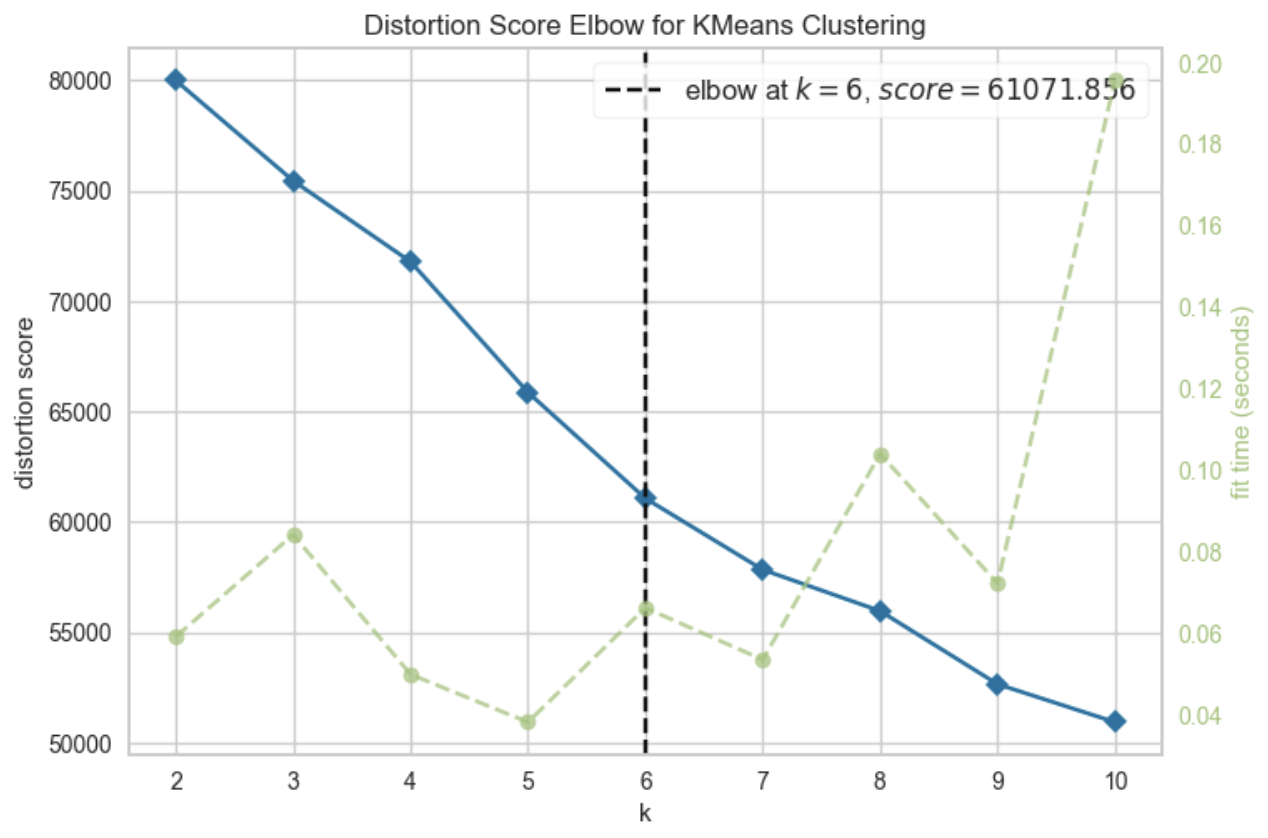
\includegraphics{kelbow.png}
\caption{Elbow Method for cluster}
\end{figure}

From this plot, it is possible to see the Eblow Plot produced by
`KElbowVisualizer'. This plot shows the distortion score on the y-axis
and the number of clusters (k) on the x-axis. The elbow is marked at k=6
with a dashed line, where the distortion score is around 61071.856,
indicating that 6 is the optimal number of clusters according to the
Elbow Method. The plot also shows the fit time for each k, which is less
relevant for determining the number of clusters but provides insight
into the computational cost.

It was also printed the centroids table that gives the average value of
each feature within each cluster, which helps in understanding the
profile of each clusters.

\begin{figure}
\centering
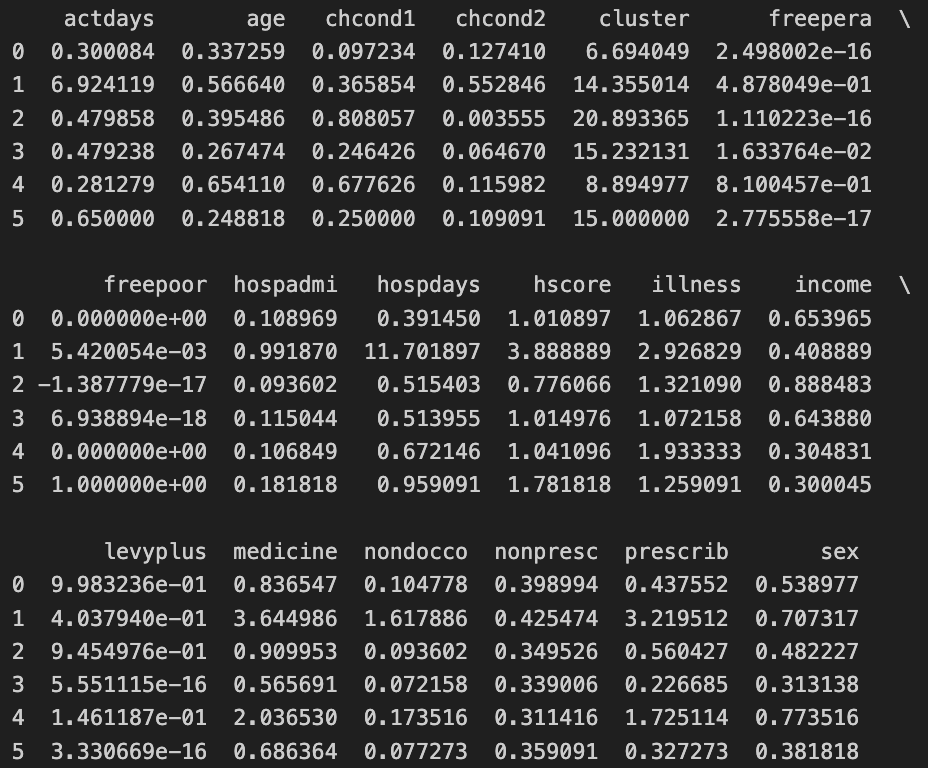
\includegraphics{centroids.png}
\caption{Centroids}
\end{figure}

For instance, Cluster 1 seems to be characterized by a higher average
`actdays' (activity limitation days) and a higher `hscore' (general
health questionnaire score), suggesting this cluster may represent
individuals with more health issues and limitations.

\subsubsection{Cluster profiling}\label{cluster-profiling}

To profile the clusters, it was examined the centroid values for each
clusters. These values gives an idea of the ``typical'' member of each
cluster.

\textbf{Cluster 0}: ``The Healthy Young Adults''

\begin{itemize}
\tightlist
\item
  Age: Younger age group.
\item
  Health: Relatively healthy with low actdays, chcond1, chcond2, and
  hscore.
\item
  Healthcare Utilization: Lower hospadmi and hospdays, indicating fewer
  hospital admissions and shorter stays.
\item
  Income: Higher than average income, possibly indicating better access
  to health resources.
\item
  Insurance: Almost all have private health insurance (levyplus).
\item
  Gender: Slightly more females than males (sex).
\end{itemize}

\textbf{Cluster 1}: ``The High-Needs Elderly''

\begin{itemize}
\tightlist
\item
  Age: Older age group.
\item
  Health: Higher actdays, chcond1, chcond2, indicating more chronic
  conditions and health issues.
\item
  Healthcare Utilization: Highest hospadmi and hospdays, suggesting
  frequent and longer hospital stays.
\item
  Income: Lower income, which could be related to retirement.
\item
  Insurance: Mixed insurance coverage.
\item
  Gender: More females than males.
\end{itemize}

\textbf{Cluster 2}: ``The Stable Middle-Aged''

\begin{itemize}
\tightlist
\item
  Age: Middle-aged group.
\item
  Health: High chcond1, but low chcond2, suggesting chronic conditions
  without severe limitations.
\item
  Healthcare Utilization: Low hospadmi and hospdays.
\item
  Income: Higher income, possibly at peak career stage.
\item
  Insurance: Mostly covered by private insurance.
\end{itemize}

\textbf{Cluster 3}: ``The Young and Occasionally Unwell''

\begin{itemize}
\tightlist
\item
  Age: Young, similar to Cluster 0.
\item
  Health: Moderate health issues, higher than Cluster 0 but less severe
  than other clusters.
\item
  Healthcare Utilization: Moderate hospadmi and hospdays.
\item
  Income: Similar to Cluster 0, relatively higher income.
\item
  Insurance: Lacks private health insurance.
\item
  Gender: More females than males.
\end{itemize}

\textbf{Cluster 4}: ``The Aging with Care Needs''

\begin{itemize}
\tightlist
\item
  Age: Older individuals, but not as old as Cluster 1.
\item
  Health: Many chronic conditions (chcond1 and chcond2).
\item
  Healthcare Utilization: Moderate hospadmi and higher hospdays.
\item
  Income: Lower income, which may impact their healthcare options.
\item
  Insurance: Some with private health insurance.
\item
  Gender: A higher proportion of females.
\end{itemize}

\textbf{Cluster 5}: ``The Economically Disadvantaged''

\begin{itemize}
\tightlist
\item
  Age: Younger, but with health issues.
\item
  Health: Moderate actdays, some chronic conditions.
\item
  Healthcare Utilization: Low to moderate hospadmi and hospdays.
\item
  Income: Low income, suggesting economic challenges.
\item
  Insurance: Lacks private health insurance, possibly relying on public
  assistance (freepoor).
\item
  Gender: Balanced gender distribution.
\end{itemize}

Each of these profiles suggests different needs and characteristics.
Strategic decisions can be made based on these insights. For example,
preventive health measures may be prioritized for clusters with chronic
conditions but not currently utilizing a lot of healthcare services
(like Cluster 2). On the other hand, policy makers may focus on
providing better economic support or healthcare access to clusters like
Cluster 5, who might be economically disadvantaged.

\subsubsection{Parallel Coordinates
Plot}\label{parallel-coordinates-plot}

The code for the following segment was done in Python (all code can be
found in the corresponding jupyter notebook).

Let's have a look at a parallel coordinates plot and see if there are
any visible patterns in the data.

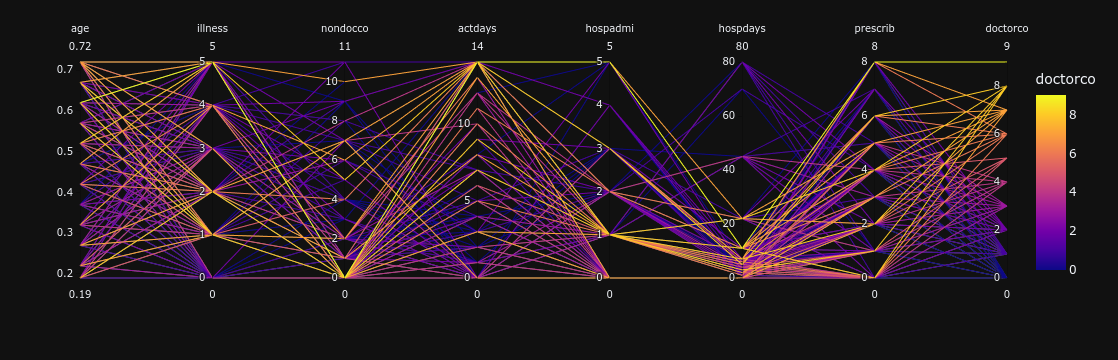
\includegraphics{pc_plot1.png}

We can take a closer look at the high values of doctors visits by
selecting just them:

\includegraphics{pc_plot2.png}

From the plots above we can draw a few conclusions. The most surprising
one is that people who visit the doctor a lot are not the same people
who stay in the hospital a lot. It seems that cases with a high number
of doctors visits may have a relatively normal length hospital stay,
after/before which they visit the doctor a lot. Interestingly, we can
also see that a lot of people with a high number of doctors visits do
get admitted to hospital at least once, if not multiple times.

Another observation is that all people with a high number of doctors
visits have been sick at least once in the past 2 weeks. We also don't
see any strong correlation between nondocco and doctorco which is
interesting. Age also doesn't seem to be a huge factor, although there
are more old people going to the doctor.

\subsubsection{Projecting the Data to 2
Dimensions}\label{projecting-the-data-to-2-dimensions}

In order to visualize the dataset with a plot, we need to reduce the
number of dimensions. It was used 2 methods for dimensionality
reduction:

\textbf{PCA}:

PCA works very well for continuous data, but our dataset is all
categorical variables, making PCA a little out of place. It should
however be interesting to see how it fares.

\textbf{MCA}:

MCA is basically PCA but for categorical data. It should work much
better for the categorical variables.

For most of this analysis, It was excluded doctors visits from the
downprojection, and instead encoding it using color. This provides a way
of analyzing how easy it may be to separate out high doctors visits from
the rest of the data.

\subsubsection{Explaining MCA}\label{explaining-mca}

MCA stands for ``Multiple Correspondence Analysis'', and is an extension
of Correspondence Analysis.

The procedure of MCA is as follows:

\begin{enumerate}
\def\labelenumi{\arabic{enumi}.}
\item
  Build an \emph{indicator matrix} (one-hot encoding of the data)
\item
  Perform CA on the indicator matrix.
\end{enumerate}

\subsubsection{Correspondence Analysis}\label{correspondence-analysis}

There are two explanations of how CA works in the context of MCA. One is
the actual regular theory, while the other is based on PCA. The regular
procedure is as follows:

\begin{enumerate}
\def\labelenumi{\arabic{enumi}.}
\tightlist
\item
  Let \(N\) be the sum of all entries in our indicator matrix \(X\).
\item
  \(Z=\frac{X}{N}\) (We're basically normalizing the data).
\item
  Let \(r\) be a vector containing the sums along the rows of \(Z\), and
  let \(c\) be the sum along all columns of \(Z\).
\item
  With this, perform the decomposition:
  \(M=diag(r)^{-\frac{1}{2}}(Z-rc^{T})diag(c)^{-\frac{1}{2}}\).
\item
  This gives you \(M=P\Delta Q^{T}\).
\end{enumerate}

\subsubsection{PCA Based Explanation}\label{pca-based-explanation}

This is the PCA based explanation:

\begin{enumerate}
\def\labelenumi{\arabic{enumi}.}
\tightlist
\item
  Let \(y_{ik}\) be a value in the indicator matrix and let \(p_{k}\) be
  the sum of row \(k\) in the indicator matrix.
\item
  We normalize the indicator matrix: \(x_{ik}=y_{ik}/p_{k} - 1\)
\item
  Apply un-standardized PCA to this matrix.
\end{enumerate}

Both of these approaches have been proven equivalent.

\subsubsection{Down-projecting with
PCA:}\label{down-projecting-with-pca}

Simply used normalized PCA on the dataset while excluding response
variable

\includegraphics{pca_down_2d.png}

The results aren't very good-looking, but it is clearly possible to see
that points with high amounts of doctors visits do stand out in some
areas. It's clear however that PCA isn't really meant for categorical
data.

\subsubsection{Down-Projecting with MCA}\label{down-projecting-with-mca}

After applying MCA, we can first have a look at the eigenvalues and
explained variance.

\begin{longtable}[]{@{}llll@{}}
\toprule\noalign{}
component & eigenvalue & \% of variance & \% of variance cumulative \\
\midrule\noalign{}
\endhead
\bottomrule\noalign{}
\endlastfoot
0 & 0.236 & 3.62\% & 3.62\% \\
1 & 0.134 & 2.05\% & 5.67\% \\
2 & 0.129 & 1.98\% & 7.64\% \\
3 & 0.115 & 1.76\% & 9.41\% \\
4 & 0.111 & 1.71\% & 11.11\% \\
5 & 0.111 & 1.70\% & 12.82\% \\
\end{longtable}

Looking at the \% of variance, this doesn't look overly promising. We
can visualize this better with a graph.

\includegraphics{mca_cumvar.png}

A note on the number of components in the graph, there are many more
components than there are dimensions in the data because when performing
MCA we have to one-hot encode the data, therefore increasing the number
of dimensions.

MCA is clearly able to remove some of the obviously correlated
dimensions such as age/agesq. However, there isn't any real elbow in the
plot. This means that reducing the number of dimensions past the very
correlated ones would lose a significant amount of information.

This is a little disappointing, however, if we were really looking to
reduce the amount of dimensions, we could choose around the 20 mark
where there is a slight bend in the curve.

\subsubsection{Visualizing the Data Using
MCA}\label{visualizing-the-data-using-mca}

\includegraphics{mca_doctors_2d.png}

This already looks a lot better than PCA, although it's difficult to see
exactly what's going on due to the overwhelming number of zero's.
Despite this, we can see that again the points with a high number of
doctors visit's do stand out a little.

\subsubsection{Looking at Different Principal
Components}\label{looking-at-different-principal-components}

Different PC's capture different elements of the data. We can explore
this by plotting them. Here we'll have a look at all combinations of the
first 3 principal components, which capture about 7.64\% percent of the
variance of the data.

\paragraph{Under-sampling the Data}\label{under-sampling-the-data}

In order to aid in visualization, was under-sampled all data by a factor
of 2, and additionally under-sampled 0's and 1's by a factor of 10. This
makes it much easier to see points with a high number of doctors visits.

\includegraphics{mca_pc_comb.png}

What is interesting about the plot above is that the best separation of
high numbers of doctors visits is being done by the 1st and 3rd
principal components. This is contrary to the fact that the 1st and 2nd
capture more variance in the data.

\subsubsection{3D Downprojection}\label{d-downprojection}

Lastly, we can also look at the projection in 3D space.

\includegraphics{mca_doctorco_3d.png}

In 3D we can clearly see that there do seem to be some clusters in the
data. However, they don't seem to be strictly related to doctors visits.

\subsubsection{Additional Data
Exploration}\label{additional-data-exploration}

In the following down-projections was included doctors visits in the
MCA. An important note is that no longer under sampling 0's and 1's
here. Instead, it is undersampling the entire dataset by a factor of 2.

\includegraphics{mca_2d_bunchofstuff.png}

The above plot's give some interesting insight into how illness, age and
income are related. We can see that the number of illnesses in the past
2 weeks is dramatically lower in young people. We can also see that
Income is much lower in older people. This makes sense as they are
probably in retirement and are not being paid a full time wage anymore.

The extreme points that seem like outliers are actually the ones with a
high number of doctors visits.

\subsubsection{Visualizing Higher Dimensional
Clusters}\label{visualizing-higher-dimensional-clusters}

The team has looked at clustering in higher dimensions, and this
down-projection gives us an opportunity to visualize these clusters.

\includegraphics{mca_clustering_vis.png}

Comparing with the previous plot's, it's interesting to be able to
directly see what kind of information these clusters have captured. For
example, the ``Aging with Care Needs'' cluster is exactly on top of
where the old population is in the dataset. This makes a lot of sense
and may even be obvious, but it's very interesting to be able to
visually see it.

We also see that a few clusters are on top of one another. This
illustrates the fact that our down-projection is inherently losing
information and is called ``overcrowding''. We knew this was a problem
based off of the explained variance presented earlier. While these
clusters may make sense in higher dimensions where there is extra
variance, they end up overlapping here.

Overcrowding is a common problem with dimensionality reduction, and it
would be interesting to be able to try some different algorithms like
t-SNE or ISOMAP, which take some extra measures over PCA to mitigate
this problem.

\section{Binary classification
problem}\label{binary-classification-problem}

We start by analyzing some models where the response variable
``doctorco'' is transformed into the binary response variable
``ifvisit''. This binary variable is equal to 0 if ``doctorco'' is 0,
and is equal to 1 otherwise. By doing so, we are modelling the number of
people that went to a doctor's visit at least once in the last two
weeks.

To start we import the data set and create the ``ifvisit'' variable.
From the following graph we can see the skewness of the data set
regarding this variable:

\includegraphics{GroupO_FinalProject_files/figure-latex/unnamed-chunk-69-1.pdf}

We can try fitting a GAM using the obtained data set:

\begin{Shaded}
\begin{Highlighting}[]
\NormalTok{model\_gam }\OtherTok{\textless{}{-}} \FunctionTok{gam}\NormalTok{(ifvisit }\SpecialCharTok{\textasciitilde{}} \FunctionTok{s}\NormalTok{(hospdays) }\SpecialCharTok{+} \FunctionTok{s}\NormalTok{(actdays) }\SpecialCharTok{+}\NormalTok{ age}\SpecialCharTok{*}\NormalTok{prescrib }\SpecialCharTok{+}\NormalTok{ freepoor }\SpecialCharTok{+}\NormalTok{ hscore }\SpecialCharTok{+}\NormalTok{ nonpresc }\SpecialCharTok{+}\NormalTok{ illness, }\AttributeTok{data =}\NormalTok{ train\_data, }\AttributeTok{family =} \FunctionTok{binomial}\NormalTok{(}\AttributeTok{link =} \StringTok{"logit"}\NormalTok{))}
\FunctionTok{summary}\NormalTok{(model\_gam)}
\end{Highlighting}
\end{Shaded}

\begin{verbatim}
## 
## Family: binomial 
## Link function: logit 
## 
## Formula:
## ifvisit ~ s(hospdays) + s(actdays) + age * prescrib + freepoor + 
##     hscore + nonpresc + illness
## 
## Parametric coefficients:
##              Estimate Std. Error z value Pr(>|z|)    
## (Intercept)  -2.72414    0.13763 -19.794  < 2e-16 ***
## age           1.52680    0.27834   5.485 4.13e-08 ***
## prescrib      0.91275    0.10486   8.704  < 2e-16 ***
## freepoor     -0.91922    0.30227  -3.041  0.00236 ** 
## hscore        0.06140    0.02004   3.064  0.00219 ** 
## nonpresc     -0.18891    0.06426  -2.940  0.00328 ** 
## illness       0.16493    0.03493   4.722 2.34e-06 ***
## age:prescrib -1.01709    0.17178  -5.921 3.20e-09 ***
## ---
## Signif. codes:  0 '***' 0.001 '**' 0.01 '*' 0.05 '.' 0.1 ' ' 1
## 
## Approximate significance of smooth terms:
##               edf Ref.df Chi.sq p-value    
## s(hospdays) 4.286  4.955  17.17 0.00514 ** 
## s(actdays)  3.259  3.931 172.31 < 2e-16 ***
## ---
## Signif. codes:  0 '***' 0.001 '**' 0.01 '*' 0.05 '.' 0.1 ' ' 1
## 
## R-sq.(adj) =  0.205   Deviance explained = 18.8%
## UBRE = -0.16331  Scale est. = 1         n = 4152
\end{verbatim}

Both the variables ``hospdays'' and ``actdays'' were considered as
splines after a top to bottom examination of the covariates. The summary
shows that we can account for approx. 19\% of explained deviance at
best, which is not a great result so far.

\begin{verbatim}
## [1] "AIC (GAM): 3473.93"
\end{verbatim}

\begin{verbatim}
## [1] "MAE (GAM): 0.1686"
\end{verbatim}

\begin{verbatim}
## [1] "Number of true ifvisit: 188"
\end{verbatim}

\begin{verbatim}
## [1] "Number of ifvisit predicted: 93"
\end{verbatim}

\includegraphics{GroupO_FinalProject_files/figure-latex/unnamed-chunk-71-1.pdf}

The sum of predicted ``ifvisit'' yealds a total of 93, against the true
value of 188, indicating that GAM isn't performing very well at
predicting the minority class `1'. To enhance it's abilities, we should
further manipulate the data set as shown in the following section.

\subsection{Balancing the data set with
ROSE}\label{balancing-the-data-set-with-rose}

Since we transformed the problem into a binary classification problem we
can use techniques to balance the data set. One option is to use ROSE
(Random Over-Sampling Examples), a method used for oversampling the
minority class in binary classification problems to balance the data
set. It involves generating synthetic examples from the existing
minority class instances. This can be achieved by randomly selecting a
minority class instance and introducing variations to create new
synthetic instances.

\begin{Shaded}
\begin{Highlighting}[]
\NormalTok{data.rose }\OtherTok{\textless{}{-}} \FunctionTok{ROSE}\NormalTok{(ifvisit }\SpecialCharTok{\textasciitilde{}}\NormalTok{ ., }\AttributeTok{data =}\NormalTok{ data, }\AttributeTok{seed =} \DecValTok{1}\NormalTok{, }\AttributeTok{hmult.majo =} \DecValTok{0}\NormalTok{)}\SpecialCharTok{$}\NormalTok{data}
\end{Highlighting}
\end{Shaded}

\includegraphics{GroupO_FinalProject_files/figure-latex/unnamed-chunk-73-1.pdf}

The ROSE method generated some data that were not suitable for the data
set, for ex. it generated negative data for variables that can only
obtain positive integer values. We solved this problem by taking the
absolute value of the data set after the data augmentation was done.

Here ROSE was first used to generate more data, then was considered the
absolute value of the dataset since the variables can't obtain negative
values, and then rounded accordingly so that every observation has
integers as values when the variable is a count.

\subsubsection{GAM with ROSE}\label{gam-with-rose}

We can try again fitting a GAM on this new balanced data set and see if
the performance improved:

\begin{Shaded}
\begin{Highlighting}[]
\NormalTok{model\_gam }\OtherTok{\textless{}{-}} \FunctionTok{gam}\NormalTok{(ifvisit }\SpecialCharTok{\textasciitilde{}} \FunctionTok{s}\NormalTok{(age) }\SpecialCharTok{+} \FunctionTok{s}\NormalTok{(actdays) }\SpecialCharTok{+} \FunctionTok{s}\NormalTok{(hscore) }\SpecialCharTok{+} \FunctionTok{s}\NormalTok{(nondocco) }\SpecialCharTok{+} \FunctionTok{s}\NormalTok{(medicine), }\AttributeTok{data=}\NormalTok{train\_data, }\AttributeTok{family =} \FunctionTok{binomial}\NormalTok{(}\AttributeTok{link =} \StringTok{"logit"}\NormalTok{))}
\FunctionTok{summary}\NormalTok{(model\_gam)}
\end{Highlighting}
\end{Shaded}

\begin{verbatim}
## 
## Family: binomial 
## Link function: logit 
## 
## Formula:
## ifvisit ~ s(age) + s(actdays) + s(hscore) + s(nondocco) + s(medicine)
## 
## Parametric coefficients:
##             Estimate Std. Error z value Pr(>|z|)   
## (Intercept)    40.91      13.05   3.135  0.00172 **
## ---
## Signif. codes:  0 '***' 0.001 '**' 0.01 '*' 0.05 '.' 0.1 ' ' 1
## 
## Approximate significance of smooth terms:
##               edf Ref.df Chi.sq p-value    
## s(age)      8.882  8.986 140.36  <2e-16 ***
## s(actdays)  8.626  8.860 596.54  <2e-16 ***
## s(hscore)   4.882  5.811  85.30  <2e-16 ***
## s(nondocco) 5.421  6.249 287.02  <2e-16 ***
## s(medicine) 6.930  7.430  49.68  <2e-16 ***
## ---
## Signif. codes:  0 '***' 0.001 '**' 0.01 '*' 0.05 '.' 0.1 ' ' 1
## 
## R-sq.(adj) =  0.843   Deviance explained = 79.4%
## UBRE = -0.69709  Scale est. = 1         n = 4152
\end{verbatim}

For this model five covariates were selected in order to predict the
response variable, those being ``actdays'', ``hscore'', ``age'',
``medicine'' and ``nondocco'', all five of them being considered as
splines. The selection was done by including all the variables and
sequentially cutting those not fit for the model.

We can appreciate a huge improvement over the previous model, getting to
a high value of approx. 80\% explained deviance.

We can see from the following plot the splines considered:

\includegraphics{GroupO_FinalProject_files/figure-latex/unnamed-chunk-76-1.pdf}

From the ``age'' spline we can infer that being ``young'' leads
generally to a moderate amount of visits, being ``adult'' leads to less
people going to the doctor, while being ``old'' implies a big chance of
going to a doctor's visit. This follows the common logic and experience,
so it's a good sign of the model working. Generally, high values of all
the covariates implies a high chance of going to the doctor, as can be
see in the previous plots.

\begin{verbatim}
## [1] "AIC (GAM): 1257.7"
\end{verbatim}

\begin{verbatim}
## [1] "MAE (GAM): 0.05491"
\end{verbatim}

\begin{verbatim}
## [1] "Number of true ifvisit: 529"
\end{verbatim}

\begin{verbatim}
## [1] "Number of ifvisit predicted: 512"
\end{verbatim}

\includegraphics{GroupO_FinalProject_files/figure-latex/unnamed-chunk-77-1.pdf}

As we can see from these results, the sum of predicted ``ifvisit'' gets
close to the true value while also maintaining a low MAE value, meaning
that the model is predicting correct values pretty consistently.

\subsubsection{GLM with ROSE}\label{glm-with-rose}

Now let's try fitting a GLM to the same balanced data set and see if it
can compete with the GAM one:

\begin{Shaded}
\begin{Highlighting}[]
\NormalTok{model\_glm }\OtherTok{\textless{}{-}} \FunctionTok{glm}\NormalTok{(ifvisit }\SpecialCharTok{\textasciitilde{}}\NormalTok{  hospadmi }\SpecialCharTok{+}\NormalTok{ nondocco }\SpecialCharTok{+}\NormalTok{ illness }\SpecialCharTok{+}\NormalTok{ actdays }\SpecialCharTok{+}\NormalTok{ prescrib }\SpecialCharTok{+}\NormalTok{ nonpresc, }\AttributeTok{data =}\NormalTok{ train\_data, }\AttributeTok{family =}\NormalTok{ binomial)}
\FunctionTok{summary}\NormalTok{(model\_glm)}
\end{Highlighting}
\end{Shaded}

\begin{verbatim}
## 
## Call:
## glm(formula = ifvisit ~ hospadmi + nondocco + illness + actdays + 
##     prescrib + nonpresc, family = binomial, data = train_data)
## 
## Coefficients:
##             Estimate Std. Error z value Pr(>|z|)    
## (Intercept) -2.58171    0.09089 -28.404  < 2e-16 ***
## hospadmi     0.95475    0.09502  10.048  < 2e-16 ***
## nondocco     1.22241    0.08169  14.965  < 2e-16 ***
## illness      0.11996    0.03324   3.609 0.000307 ***
## actdays      0.53808    0.02988  18.005  < 2e-16 ***
## prescrib     0.47077    0.03747  12.563  < 2e-16 ***
## nonpresc     0.25345    0.05829   4.348 1.37e-05 ***
## ---
## Signif. codes:  0 '***' 0.001 '**' 0.01 '*' 0.05 '.' 0.1 ' ' 1
## 
## (Dispersion parameter for binomial family taken to be 1)
## 
##     Null deviance: 5749.9  on 4151  degrees of freedom
## Residual deviance: 2947.5  on 4145  degrees of freedom
## AIC: 2961.5
## 
## Number of Fisher Scoring iterations: 6
\end{verbatim}

Firstly, we can see that the AIC is two times the AIC from the GAM
model. Furthermore, the explained deviance is at best around 50\%, which
is a better result but still not as good as GAM.

\begin{verbatim}
## [1] "MAE (GLM): 0.1021"
\end{verbatim}

\begin{verbatim}
## [1] "Number of true ifvisit: 529"
\end{verbatim}

\begin{verbatim}
## [1] "Number of ifvisit predicted: 499"
\end{verbatim}

\includegraphics{GroupO_FinalProject_files/figure-latex/unnamed-chunk-79-1.pdf}

From the obtained results we can see that GAM manages to find a good
approximation of the total number of visits while also keeping a low
value of MAE, meaning that the predictions are correct most of the
times.

On the other hand, GLM is a little worse at predicting the total number
of visits (sum of ``ifvisit'') and it scores double the MAE from GAM
meaning that the predictions are overall worse but still useful. GAM
manages to understand better the variable interactions but GLM is faster
and simpler to interpret.

From this analysis we can say that augmenting a skewed data set such as
the one we are analyzing can improve and ease the binary classification
problem, and also that the GAM model is much better, in this particular
data set, at accurately predicting if a person has gone to the doctor in
the past two weeks or not.

This concludes the binary classification digression, from now on all the
models will try to predict the whole ``doctorco'' variable.

\section{ZERO INFLATED NEGATIVE
BINOMIAL}\label{zero-inflated-negative-binomial}

Traditional Negative Binomial regression extends Poisson regression to
manage overdispersion in count data, but it fails when an unusually high
number of zero counts is present. The ZINB model is combining the
principles of NB regression with a mechanism to account for excess
zeros. Specifically, it differentiates between two sources of zeros:
those arising from the data's natural variability ``sampling zeros'' and
those that are structurally inherent or ``excess zeros.''

\[
P(Y_i = y_i) = \left\{
    \begin{array}{ll}
        \pi_i + (1 - \pi_i) \frac{\Gamma(r + y_i)}{\Gamma(r) y_i!} \left(\frac{r}{r + \mu_i}\right)^r \left(\frac{\mu_i}{r + \mu_i}\right)^{y_i} & \mbox{if } y_i = 0, \\
        (1 - \pi_i) \frac{\Gamma(r + y_i)}{\Gamma(r) y_i!} \left(\frac{r}{r + \mu_i}\right)^r \left(\frac{\mu_i}{r + \mu_i}\right)^{y_i} & \mbox{if } y_i > 0.
    \end{array}
\right.
\]

The ZINB model accounts for the excess of zeros through the component
\(\pi_i\), which represents the probability that an observation will
have a count of zero not due to the process described by the Negative
Binomial distribution but due to some other, external process. Another
key feature is the dispersion parameter \(r\) of the Negative Binomial
distribution, which is used to model overdispersion. Smaller values of
\(r\) indicate greater overdispersion relative to the Poisson
distribution.

We use the model `zeroinfl' that has two parts:

\begin{itemize}
\item left of the | symbol: Specifies the variables for the count model part. This part models the actual count of doctor visits based on predictors such as illness, actdays, hscore, chcond1, age:chcond2, hospadmi, prescrib, and nonpresc.
\item right of the | symbol: Specifies the variables for the zero-inflation model part. This part models the excess zeros, predicting which zeros are "true zeros". Here, predictors like levyplus, age:income:freepoor, freepera, and interactions are used.
\end{itemize}

\begin{Shaded}
\begin{Highlighting}[]
\NormalTok{ZINB\_model }\OtherTok{\textless{}{-}} \FunctionTok{zeroinfl}\NormalTok{(doctorco }\SpecialCharTok{\textasciitilde{}}\NormalTok{illness }\SpecialCharTok{*}\NormalTok{ actdays }\SpecialCharTok{+}\NormalTok{ hscore }\SpecialCharTok{+}\NormalTok{ chcond1 }\SpecialCharTok{+}\NormalTok{ age}\SpecialCharTok{:}\NormalTok{ chcond2 }
\SpecialCharTok{+}\NormalTok{ hospadmi  }\SpecialCharTok{+}\NormalTok{ prescrib }\SpecialCharTok{+}\NormalTok{ nonpresc}\SpecialCharTok{|}\NormalTok{levyplus }\SpecialCharTok{+}\NormalTok{ age}\SpecialCharTok{:}\NormalTok{income}\SpecialCharTok{:}\NormalTok{freepoor }\SpecialCharTok{+}\NormalTok{ freepera}
\SpecialCharTok{+}\NormalTok{ illness }\SpecialCharTok{*}\NormalTok{ actdays }\SpecialCharTok{+}\NormalTok{ prescrib, }\AttributeTok{data =}\NormalTok{ train\_data, }\AttributeTok{dist =} \StringTok{"negbin"}\NormalTok{)}

\FunctionTok{AIC}\NormalTok{(ZINB\_model)}
\end{Highlighting}
\end{Shaded}

\begin{verbatim}
## [1] 4908.415
\end{verbatim}

\begin{Shaded}
\begin{Highlighting}[]
\FunctionTok{summary}\NormalTok{(ZINB\_model)}
\end{Highlighting}
\end{Shaded}

\begin{verbatim}
## 
## Call:
## zeroinfl(formula = doctorco ~ illness * actdays + hscore + chcond1 + 
##     age:chcond2 + hospadmi + prescrib + nonpresc | levyplus + age:income:freepoor + 
##     freepera + illness * actdays + prescrib, data = train_data, dist = "negbin")
## 
## Pearson residuals:
##     Min      1Q  Median      3Q     Max 
## -1.2568 -0.4370 -0.2498 -0.1729 11.1233 
## 
## Count model coefficients (negbin with log link):
##                  Estimate Std. Error z value Pr(>|z|)    
## (Intercept)     -0.958567   0.132317  -7.244 4.34e-13 ***
## illness          0.097356   0.035625   2.733 0.006280 ** 
## actdays          0.101887   0.013337   7.640 2.18e-14 ***
## hscore           0.024368   0.013309   1.831 0.067112 .  
## chcond11        -0.149808   0.088641  -1.690 0.091017 .  
## hospadmi         0.185576   0.044157   4.203 2.64e-05 ***
## prescrib         0.082195   0.024279   3.385 0.000711 ***
## nonpresc        -0.151691   0.048728  -3.113 0.001852 ** 
## illness:actdays -0.007148   0.004526  -1.579 0.114245    
## age:chcond20    -0.209779   0.209290  -1.002 0.316183    
## age:chcond21    -0.624787   0.240798  -2.595 0.009469 ** 
## Log(theta)       0.893182   0.165991   5.381 7.41e-08 ***
## 
## Zero-inflation model coefficients (binomial with logit link):
##                      Estimate Std. Error z value Pr(>|z|)    
## (Intercept)            1.8827     0.2604   7.231 4.79e-13 ***
## levyplus1             -0.4330     0.2189  -1.978 0.047921 *  
## freepera1             -1.5382     0.3749  -4.103 4.07e-05 ***
## illness               -0.4317     0.1119  -3.856 0.000115 ***
## actdays               -2.3676     0.8194  -2.890 0.003857 ** 
## prescrib              -1.6775     0.2515  -6.669 2.57e-11 ***
## illness:actdays        0.4764     0.1719   2.772 0.005567 ** 
## age:income:freepoor0   0.2498     0.6597   0.379 0.704958    
## age:income:freepoor1  20.5385     8.8031   2.333 0.019643 *  
## ---
## Signif. codes:  0 '***' 0.001 '**' 0.01 '*' 0.05 '.' 0.1 ' ' 1 
## 
## Theta = 2.4429 
## Number of iterations in BFGS optimization: 72 
## Log-likelihood: -2433 on 21 Df
\end{verbatim}

There are significant variables that influence the number of doctor
visits. Notably, income factors (both middle and high income showing
lower visit rates compared to low-income counterparts), levyplus,
health-related variables like illness severity, active days, and
hospital admissions directly correlate with increased doctor visits,
emphasizing the link between health needs and healthcare demand.
Prescription medication requirements further elevate visit frequencies,
reflecting ongoing health management needs. Conversely, the use of
non-prescription medications is associated with fewer visits, hinting at
self-care practices for minor health concerns.

The interaction term age:income:freepoor1 and its significant positive
coefficient suggest that older individuals with higher income who
qualify for free healthcare are less likely to visit the doctor. This
pattern may arise from various factors such as improved health status,
access to alternative health resources, or specific policies that affect
their healthcare utilization differently. Additionally, the interaction
between illness and actdays demonstrates a significant positive effect,
indicating that individuals who are ill and experience more days of
activity restriction are more likely to seek medical attention, which
aligns with expectations.

In the zero-inflation part, variables like levyplus, freepera, illness,
actdays, and prescrib are significant, pointing to specific factors that
influence the propensity to have zero visits.

Theta is a parameter of the Negative Binomial distribution part of the
model it is inversely related to the variance; a smaller \(\theta\)
indicates more dispersion (more variability in count data than what a
Poisson model would suggest). Theta of 2.4 suggests some level of
overdispersion in the data, but not extremely high.

\begin{Shaded}
\begin{Highlighting}[]
\NormalTok{predicted\_counts\_zinb }\OtherTok{\textless{}{-}} \FunctionTok{round}\NormalTok{(}\FunctionTok{predict}\NormalTok{(ZINB\_model, }\AttributeTok{newdata =}\NormalTok{ test\_data, }\AttributeTok{type =} \StringTok{"response"}\NormalTok{))}
\NormalTok{predicted\_category\_zinb }\OtherTok{\textless{}{-}} \FunctionTok{ifelse}\NormalTok{(predicted\_counts\_zinb }\SpecialCharTok{\textless{}} \DecValTok{1}\NormalTok{, }\DecValTok{0}\NormalTok{,predicted\_counts\_zinb)}

\NormalTok{true\_counts }\OtherTok{\textless{}{-}}\NormalTok{ test\_data}\SpecialCharTok{$}\NormalTok{doctorco}
\NormalTok{mae\_zinb }\OtherTok{\textless{}{-}} \FunctionTok{mean}\NormalTok{(}\FunctionTok{abs}\NormalTok{(predicted\_counts\_zinb }\SpecialCharTok{{-}}\NormalTok{ true\_counts))}
\FunctionTok{cat}\NormalTok{(}\StringTok{"MAE:"}\NormalTok{, mae\_zinb, }\StringTok{"}\SpecialCharTok{\textbackslash{}n}\StringTok{"}\NormalTok{)}
\end{Highlighting}
\end{Shaded}

\begin{verbatim}
## MAE: 0.2649326
\end{verbatim}

\begin{Shaded}
\begin{Highlighting}[]
\NormalTok{rmse\_zinb }\OtherTok{\textless{}{-}} \FunctionTok{sqrt}\NormalTok{(}\FunctionTok{mean}\NormalTok{((predicted\_counts\_zinb }\SpecialCharTok{{-}}\NormalTok{ true\_counts)}\SpecialCharTok{\^{}}\DecValTok{2}\NormalTok{))}
\FunctionTok{cat}\NormalTok{(}\StringTok{"RMSE:"}\NormalTok{, rmse\_zinb, }\StringTok{"}\SpecialCharTok{\textbackslash{}n}\StringTok{"}\NormalTok{)}
\end{Highlighting}
\end{Shaded}

\begin{verbatim}
## RMSE: 0.6988843
\end{verbatim}

The modelsts Mean Absolute Error (MAE) is indicating a relatively
precise prediction capability given the context of count data; but still
has room for improvement, particularly in accurately predicting higher
counts of visits as seen from the Root Mean Squared Error (RMSE).

This section explores the examination of binary outcomes---specifically,
the presence or absence of doctor visits. By utilizing confusion
matrices and metrics such as balanced accuracy and AUC-ROC, we want to
evaluate the model's ability to accurately predict actual visits against
the backdrop of a skewed distribution.

\begin{verbatim}
## Confusion Matrix and Statistics
## 
##           Reference
## Prediction   0   1
##          0 778 104
##          1  72  84
##                                           
##                Accuracy : 0.8304          
##                  95% CI : (0.8062, 0.8528)
##     No Information Rate : 0.8189          
##     P-Value [Acc > NIR] : 0.17730         
##                                           
##                   Kappa : 0.3878          
##                                           
##  Mcnemar's Test P-Value : 0.01945         
##                                           
##             Sensitivity : 0.9153          
##             Specificity : 0.4468          
##          Pos Pred Value : 0.8821          
##          Neg Pred Value : 0.5385          
##              Prevalence : 0.8189          
##          Detection Rate : 0.7495          
##    Detection Prevalence : 0.8497          
##       Balanced Accuracy : 0.6811          
##                                           
##        'Positive' Class : 0               
## 
\end{verbatim}

\begin{verbatim}
## Balanced Accuracy: 0.5384615
\end{verbatim}

\begin{verbatim}
## Setting levels: control = 0, case = 1
\end{verbatim}

\begin{verbatim}
## Setting direction: controls < cases
\end{verbatim}

\begin{verbatim}
## AUC-ROC: 0.6810513
\end{verbatim}

The high accuracy indicates that almost all predictions made by the
model are correct. This is a relatively high overall accuracy rate. The
sensitivity of reflects the model's strong performance in predicting
non-visits accurately, a result of the data's inherent imbalance towards
this outcome.

However, the model's balanced accuracy and an AUC-ROC score suggest that
while the model is better than a dummy classifier, there is room for
improvement, particularly in correctly identifying actual visits.

By plotting distribution of both actual and predicted visits, we gain
insights into the model's performance in capturing the true distribution
of healthcare utilization. Additionally, examining the specific actual
versus predicted counts across visit frequencies enables us to identify
where the model performs well.

\begin{Shaded}
\begin{Highlighting}[]
\NormalTok{actual\_freq }\OtherTok{\textless{}{-}} \FunctionTok{table}\NormalTok{(true\_counts)}
\NormalTok{predicted\_freq\_zinb }\OtherTok{\textless{}{-}} \FunctionTok{table}\NormalTok{(predicted\_counts\_zinb)}

\FunctionTok{par}\NormalTok{(}\AttributeTok{mfrow=}\FunctionTok{c}\NormalTok{(}\DecValTok{1}\NormalTok{,}\DecValTok{2}\NormalTok{))}

\CommentTok{\# Bar plot for Actual Counts}
\FunctionTok{barplot}\NormalTok{(actual\_freq, }\AttributeTok{main=}\StringTok{"Actual Visits"}\NormalTok{, }\AttributeTok{xlab=}\StringTok{"Doctor Visits Count"}\NormalTok{,}
        \AttributeTok{ylab=}\StringTok{"Frequency"}\NormalTok{, }\AttributeTok{col=}\StringTok{"lightblue"}\NormalTok{)}

\CommentTok{\# Bar plot for Predicted Counts}
\FunctionTok{barplot}\NormalTok{(predicted\_freq\_zinb, }\AttributeTok{main=}\StringTok{"Predicted Visits"}\NormalTok{, }\AttributeTok{xlab=}\StringTok{"Predicted Visits Count"}\NormalTok{,}
        \AttributeTok{ylab=}\StringTok{"Frequency"}\NormalTok{, }\AttributeTok{col=}\StringTok{"darkblue"}\NormalTok{)}
\end{Highlighting}
\end{Shaded}

\includegraphics{GroupO_FinalProject_files/figure-latex/unnamed-chunk-84-1.pdf}

\begin{Shaded}
\begin{Highlighting}[]
\FunctionTok{par}\NormalTok{(}\AttributeTok{mfrow=}\FunctionTok{c}\NormalTok{(}\DecValTok{1}\NormalTok{,}\DecValTok{1}\NormalTok{))}


\ControlFlowTok{for}\NormalTok{ (i }\ControlFlowTok{in} \DecValTok{0}\SpecialCharTok{:}\DecValTok{9}\NormalTok{) \{}
\NormalTok{  actual\_ }\OtherTok{\textless{}{-}}\NormalTok{ true\_counts }\SpecialCharTok{==}\NormalTok{ i}
\NormalTok{  predicted\_ }\OtherTok{\textless{}{-}}\NormalTok{ predicted\_counts\_zinb }\SpecialCharTok{==}\NormalTok{ i}
\NormalTok{  actual\_count }\OtherTok{\textless{}{-}} \FunctionTok{sum}\NormalTok{(actual\_)}
\NormalTok{  predicted\_count}\OtherTok{\textless{}{-}} \FunctionTok{sum}\NormalTok{(predicted\_)}
  \FunctionTok{cat}\NormalTok{(}\StringTok{"Actual count for"}\NormalTok{, i, }\StringTok{"Visits:"}\NormalTok{, actual\_count, }\StringTok{"}\SpecialCharTok{\textbackslash{}n}\StringTok{"}\NormalTok{)}
  \FunctionTok{cat}\NormalTok{(}\StringTok{"Predicted count for"}\NormalTok{, i, }\StringTok{"Visits:"}\NormalTok{, predicted\_count, }\StringTok{"}\SpecialCharTok{\textbackslash{}n\textbackslash{}n}\StringTok{"}\NormalTok{)}
\NormalTok{\}}
\end{Highlighting}
\end{Shaded}

\begin{verbatim}
## Actual count for 0 Visits: 850 
## Predicted count for 0 Visits: 882 
## 
## Actual count for 1 Visits: 142 
## Predicted count for 1 Visits: 134 
## 
## Actual count for 2 Visits: 29 
## Predicted count for 2 Visits: 16 
## 
## Actual count for 3 Visits: 5 
## Predicted count for 3 Visits: 4 
## 
## Actual count for 4 Visits: 4 
## Predicted count for 4 Visits: 1 
## 
## Actual count for 5 Visits: 2 
## Predicted count for 5 Visits: 1 
## 
## Actual count for 6 Visits: 2 
## Predicted count for 6 Visits: 0 
## 
## Actual count for 7 Visits: 3 
## Predicted count for 7 Visits: 0 
## 
## Actual count for 8 Visits: 1 
## Predicted count for 8 Visits: 0 
## 
## Actual count for 9 Visits: 0 
## Predicted count for 9 Visits: 0
\end{verbatim}

The model does well at predicting when there are no doctor visits,
although it predicts slightly more zeros than there actually are.
However, as the number of visits goes up, the model does not do as well.
It is close when predicting one visit but starts to fall short with two
visits and struggles more as the visit numbers increase, not predicting
any visits of five or more at all. This gap between the actual and
predicted numbers, especially for higher counts of visits, suggests that
the model might need some improvements or additional data to better
predict these less common situations.

\section{HURDLE NEGATIVE BINOMIAL}\label{hurdle-negative-binomial}

The hurdle model offers a distinct approach to modeling count data,
unlike Zero-Inflated models, hurdle models decompose the prediction
process into two sequential components: a binary process for
distinguishing between zero and non-zero counts, followed by a truncated
count distribution model exclusively for the positive counts. This
structure creates a ``hurdle'' that separates zero predictions from
positive ones, meaning observations must first cross this hurdle before
they are considered for positive count predictions.

In the hurdle model framework, the probability of observing a zero count
(\(y_i = 0\)) is denoted by \(p_i\), while the distribution of positive
counts (\(y_i > 0\)) follows a truncated distribution, adjusted to
exclude the probability of zero counts. The mathematical representation
of the HNB model is as follows:

\[
P(Y_i = y_i) = 
\begin{cases} 
p_i & \text{if } y_i = 0, \\
(1 - p_i) \frac{p(y_i; \mu_i)}{1 - p(y_i = 0; \mu_i)} & \text{if } y_i > 0,
\end{cases}
\]

Here, \(p_i\) delineates the probability that an observation falls into
the zero count category, while \(p(y_i; \mu_i)\) denotes the probability
mass function (PMF) for positive counts, parameterized by \(\mu_i\),
within a Negative Binomial distribution managing the observed
overdispersion in the data.

The HNB model separates the prediction of no visits from the prediction
of one or more visits to better understand healthcare usage. It first
decides if a visit happens at all and then predicts how many visits will
happen if it does. The model uses different factors to predict both the
chance of no visits and the expected number of visits, helping us
understand what influences these outcomes.

The hurdle model implemented with the `pscl' library in R is designed
dividing the modeling process into two distinct parts separated by
`\textbar{}'.

\begin{Shaded}
\begin{Highlighting}[]
\NormalTok{hurdle\_model }\OtherTok{\textless{}{-}} \FunctionTok{hurdle}\NormalTok{(doctorco }\SpecialCharTok{\textasciitilde{}}\NormalTok{ illness }\SpecialCharTok{+}\NormalTok{ actdays }\SpecialCharTok{+}\NormalTok{ hospadmi}\SpecialCharTok{|}\NormalTok{income}\SpecialCharTok{:}\NormalTok{freepoor }\SpecialCharTok{+} 
\NormalTok{                         actdays }\SpecialCharTok{*}\NormalTok{illness }\SpecialCharTok{+}\NormalTok{ sex}\SpecialCharTok{*}\NormalTok{hscore }\SpecialCharTok{+}\NormalTok{ hospadmi }\SpecialCharTok{+}\NormalTok{ prescrib }\SpecialCharTok{+}\NormalTok{ nonpresc,}
                       \AttributeTok{data =}\NormalTok{ train\_data, }\AttributeTok{dist =}\StringTok{"negbin"}\NormalTok{)}

\FunctionTok{AIC}\NormalTok{(hurdle\_model)}
\end{Highlighting}
\end{Shaded}

\begin{verbatim}
## [1] 4980.611
\end{verbatim}

\begin{Shaded}
\begin{Highlighting}[]
\CommentTok{\#summary(hurdle\_model)}

\CommentTok{\#hurdle with factors}
\NormalTok{hurdle\_model2 }\OtherTok{\textless{}{-}} \FunctionTok{hurdle}\NormalTok{(doctorco }\SpecialCharTok{\textasciitilde{}}\NormalTok{ income\_factor}\SpecialCharTok{+}\NormalTok{illness }\SpecialCharTok{+}\NormalTok{  actdays}\SpecialCharTok{+}\NormalTok{ hospadmi}\SpecialCharTok{|}
\NormalTok{                          income}\SpecialCharTok{:}\NormalTok{freepoor }\SpecialCharTok{+}\NormalTok{ actdays }\SpecialCharTok{*}\NormalTok{illness }\SpecialCharTok{+}\NormalTok{ sex}\SpecialCharTok{*}\NormalTok{hscore }\SpecialCharTok{+}\NormalTok{ hospadmi }\SpecialCharTok{+}
\NormalTok{                          age\_factor}\SpecialCharTok{*}\NormalTok{prescrib }\SpecialCharTok{+}\NormalTok{ nonpresc,}
                        \AttributeTok{data =}\NormalTok{ train\_data, }\AttributeTok{dist =} \StringTok{"negbin"}\NormalTok{)}

\FunctionTok{AIC}\NormalTok{(hurdle\_model2)}
\end{Highlighting}
\end{Shaded}

\begin{verbatim}
## [1] 4921.703
\end{verbatim}

Key findings from the model coefficients suggest that factors such as
income level, illness severity, the number of activity days, hospital
admissions, and prescription medication usage significantly influence
both the likelihood of making any doctor visit and the frequency of
those visits among patients who do.

Notably, the interaction terms, such sex with health score, underscore
how the combined effect of these variables can either increase or
decrease the likelihood of seeking medical care. For instance, the
significant negative coefficient for the interaction between income and
freepoor1 suggests that patients from lower-income brackets with access
to free poor services are less likely to have zero visits, indicating
targeted healthcare access among vulnerable populations.

The theta value, reported as 0.1933 in the count model, is indicative of
the degree of overdispersion relative to what a Poisson distribution
would predict. A theta value significantly lower than 1 points towards
high overdispersion, validating the choice of a negative binomial
distribution over a Poisson.

\begin{Shaded}
\begin{Highlighting}[]
\NormalTok{predicted\_counts\_hurdle }\OtherTok{\textless{}{-}} \FunctionTok{round}\NormalTok{(}\FunctionTok{predict}\NormalTok{(hurdle\_model2, }\AttributeTok{newdata=}\NormalTok{test\_data, }\AttributeTok{type =} \StringTok{"response"}\NormalTok{))}
\NormalTok{predicted\_category\_hnb }\OtherTok{\textless{}{-}} \FunctionTok{ifelse}\NormalTok{(predicted\_counts\_hurdle}\SpecialCharTok{\textless{}} \DecValTok{1}\NormalTok{, }\DecValTok{0}\NormalTok{, predicted\_counts\_hurdle)}


\NormalTok{true\_counts }\OtherTok{\textless{}{-}}\NormalTok{ test\_data}\SpecialCharTok{$}\NormalTok{doctorco}
\NormalTok{mae\_hurdle }\OtherTok{\textless{}{-}} \FunctionTok{mean}\NormalTok{(}\FunctionTok{abs}\NormalTok{(predicted\_counts\_hurdle}\SpecialCharTok{{-}}\NormalTok{ true\_counts))}
\FunctionTok{cat}\NormalTok{(}\StringTok{"MAE:"}\NormalTok{, mae\_hurdle, }\StringTok{"}\SpecialCharTok{\textbackslash{}n}\StringTok{"}\NormalTok{)}
\end{Highlighting}
\end{Shaded}

\begin{verbatim}
## MAE: 0.283237
\end{verbatim}

\begin{Shaded}
\begin{Highlighting}[]
\NormalTok{rmse\_hurdle }\OtherTok{\textless{}{-}} \FunctionTok{sqrt}\NormalTok{(}\FunctionTok{mean}\NormalTok{((predicted\_counts\_hurdle }\SpecialCharTok{{-}}\NormalTok{ true\_counts)}\SpecialCharTok{\^{}}\DecValTok{2}\NormalTok{))}
\FunctionTok{cat}\NormalTok{(}\StringTok{"RMSE:"}\NormalTok{, rmse\_hurdle, }\StringTok{"}\SpecialCharTok{\textbackslash{}n}\StringTok{"}\NormalTok{)}
\end{Highlighting}
\end{Shaded}

\begin{verbatim}
## RMSE: 0.7602859
\end{verbatim}

The MAE indicates a relatively small deviation, suggesting that the
model's predictions are, on average, close to the true number of visits.
The RMSE, which penalizes larger errors more heavily, is higher,
suggesting that there are some instances of larger prediction errors,
but overall, the model demonstrates a decent level of accuracy.

Also for the hurdle model, we evaluate alternative metrics for the
binary outcome, focusing on the dichotomy of having or not having doctor
visits. Employing confusion matrices, balanced accuracy, and AUC-ROC,
this analysis aims to assess the model's precision in distinguishing
actual visits in a dataset significantly skewed towards non-visits.

\begin{Shaded}
\begin{Highlighting}[]
\NormalTok{actual\_binary }\OtherTok{\textless{}{-}} \FunctionTok{ifelse}\NormalTok{(true\_counts }\SpecialCharTok{\textgreater{}} \DecValTok{0}\NormalTok{, }\DecValTok{1}\NormalTok{, }\DecValTok{0}\NormalTok{)}
\NormalTok{predicted\_binary }\OtherTok{\textless{}{-}} \FunctionTok{ifelse}\NormalTok{(predicted\_counts\_hurdle }\SpecialCharTok{\textgreater{}} \DecValTok{0}\NormalTok{, }\DecValTok{1}\NormalTok{, }\DecValTok{0}\NormalTok{)}
\NormalTok{conf\_matrix }\OtherTok{\textless{}{-}} \FunctionTok{table}\NormalTok{(}\AttributeTok{Actual =}\NormalTok{ actual\_binary, }\AttributeTok{Predicted =}\NormalTok{ predicted\_binary)}
\FunctionTok{confusionMatrix}\NormalTok{(}\FunctionTok{as.factor}\NormalTok{(predicted\_binary), }\FunctionTok{as.factor}\NormalTok{(actual\_binary))}
\end{Highlighting}
\end{Shaded}

\begin{verbatim}
## Confusion Matrix and Statistics
## 
##           Reference
## Prediction   0   1
##          0 788 124
##          1  62  64
##                                           
##                Accuracy : 0.8208          
##                  95% CI : (0.7961, 0.8437)
##     No Information Rate : 0.8189          
##     P-Value [Acc > NIR] : 0.4552          
##                                           
##                   Kappa : 0.3069          
##                                           
##  Mcnemar's Test P-Value : 7.722e-06       
##                                           
##             Sensitivity : 0.9271          
##             Specificity : 0.3404          
##          Pos Pred Value : 0.8640          
##          Neg Pred Value : 0.5079          
##              Prevalence : 0.8189          
##          Detection Rate : 0.7592          
##    Detection Prevalence : 0.8786          
##       Balanced Accuracy : 0.6337          
##                                           
##        'Positive' Class : 0               
## 
\end{verbatim}

\begin{Shaded}
\begin{Highlighting}[]
\CommentTok{\# Balanced accuracy}
\NormalTok{balanced\_accuracy }\OtherTok{\textless{}{-}}\NormalTok{ (}\FunctionTok{sensitivity}\NormalTok{(conf\_matrix, }\AttributeTok{positive =} \StringTok{"1"}\NormalTok{) }\SpecialCharTok{+}
                        \FunctionTok{specificity}\NormalTok{(conf\_matrix, }\AttributeTok{positive =} \StringTok{"1"}\NormalTok{)) }\SpecialCharTok{/} \DecValTok{2}
\FunctionTok{cat}\NormalTok{(}\StringTok{"Balanced Accuracy:"}\NormalTok{, balanced\_accuracy, }\StringTok{"}\SpecialCharTok{\textbackslash{}n}\StringTok{"}\NormalTok{)}
\end{Highlighting}
\end{Shaded}

\begin{verbatim}
## Balanced Accuracy: 0.5079365
\end{verbatim}

\begin{Shaded}
\begin{Highlighting}[]
\CommentTok{\# AUC{-}ROC}
\NormalTok{roc\_result }\OtherTok{\textless{}{-}} \FunctionTok{roc}\NormalTok{(actual\_binary, }\FunctionTok{as.numeric}\NormalTok{(predicted\_binary) }\SpecialCharTok{{-}} \DecValTok{1}\NormalTok{)}
\end{Highlighting}
\end{Shaded}

\begin{verbatim}
## Setting levels: control = 0, case = 1
\end{verbatim}

\begin{verbatim}
## Setting direction: controls < cases
\end{verbatim}

\begin{Shaded}
\begin{Highlighting}[]
\NormalTok{auc\_roc }\OtherTok{\textless{}{-}} \FunctionTok{auc}\NormalTok{(roc\_result)}
\FunctionTok{cat}\NormalTok{(}\StringTok{"AUC{-}ROC:"}\NormalTok{, auc\_roc, }\StringTok{"}\SpecialCharTok{\textbackslash{}n}\StringTok{"}\NormalTok{)}
\end{Highlighting}
\end{Shaded}

\begin{verbatim}
## AUC-ROC: 0.6337422
\end{verbatim}

The confusion matrix generated from this analysis revealed that the
model correctly predicted 788 instances with no visits and 66 instances
where visits occurred, against 62 false positives and 122 false
negatives. This resulted in a high accuracy rate, a figure slightly
higher than the no information rate, indicating the model's predictive
capability beyond random chance, albeit with room for improvement,
particularly in correctly identifying positive instances.

The model demonstrated a high sensitivity, indicating a strong ability
to correctly identify true negatives, but a lower specificity,
reflecting challenges in accurately predicting true positives. The
balanced accuracy, an average of sensitivity and specificity is
suggesting a need to enhance the model's ability to balance both types
of correct predictions. The Area Under the Receiver Operating
Characteristic curve (AUC-ROC) is showcasing the model's fair
discrimination ability between zero and non-zero visit

The model is adept at identifying a significant portion of the
non-visits (as evidenced by high sensitivity), it struggles more with
accurately predicting actual visits (reflected in lower specificity and
NPV). This can happen if the model better captures the zero-inflation
aspect but less so the count distribution among the positive outcomes.
in the following part we will take a look at how the model predicts the
count part of the model.

\begin{Shaded}
\begin{Highlighting}[]
\NormalTok{actual\_freq }\OtherTok{\textless{}{-}} \FunctionTok{table}\NormalTok{(true\_counts)}
\NormalTok{predicted\_freq }\OtherTok{\textless{}{-}} \FunctionTok{table}\NormalTok{(predicted\_counts\_hurdle)}

\FunctionTok{par}\NormalTok{(}\AttributeTok{mfrow=}\FunctionTok{c}\NormalTok{(}\DecValTok{1}\NormalTok{,}\DecValTok{2}\NormalTok{))}

\CommentTok{\# Bar plot for Actual Counts}
\FunctionTok{barplot}\NormalTok{(actual\_freq, }\AttributeTok{main=}\StringTok{"Actual Visits"}\NormalTok{, }\AttributeTok{xlab=}\StringTok{"Doctor Visits Count"}\NormalTok{,}
        \AttributeTok{ylab=}\StringTok{"Frequency"}\NormalTok{, }\AttributeTok{col=}\StringTok{"lightblue"}\NormalTok{)}

\CommentTok{\# Bar plot for Predicted Counts}
\FunctionTok{barplot}\NormalTok{(predicted\_freq, }\AttributeTok{main=}\StringTok{"Predicted Visits"}\NormalTok{, }\AttributeTok{xlab=}\StringTok{"Predicted Visits Count"}\NormalTok{, }
        \AttributeTok{ylab=}\StringTok{"Frequency"}\NormalTok{, }\AttributeTok{col=}\StringTok{"darkblue"}\NormalTok{)}
\end{Highlighting}
\end{Shaded}

\includegraphics{GroupO_FinalProject_files/figure-latex/unnamed-chunk-87-1.pdf}

\begin{Shaded}
\begin{Highlighting}[]
\FunctionTok{par}\NormalTok{(}\AttributeTok{mfrow=}\FunctionTok{c}\NormalTok{(}\DecValTok{1}\NormalTok{,}\DecValTok{1}\NormalTok{))}

\ControlFlowTok{for}\NormalTok{ (i }\ControlFlowTok{in} \DecValTok{0}\SpecialCharTok{:}\DecValTok{9}\NormalTok{) \{}
\NormalTok{  actual\_ }\OtherTok{\textless{}{-}}\NormalTok{ true\_counts }\SpecialCharTok{==}\NormalTok{ i}
\NormalTok{  predicted\_ }\OtherTok{\textless{}{-}}\NormalTok{ predicted\_counts\_hurdle }\SpecialCharTok{==}\NormalTok{ i}
\NormalTok{  actual\_count }\OtherTok{\textless{}{-}} \FunctionTok{sum}\NormalTok{(actual\_)}
\NormalTok{  predicted\_count }\OtherTok{\textless{}{-}} \FunctionTok{sum}\NormalTok{(predicted\_)}
  \FunctionTok{cat}\NormalTok{(}\StringTok{"Actual count for"}\NormalTok{, i, }\StringTok{"Visits:"}\NormalTok{, actual\_count, }\StringTok{"}\SpecialCharTok{\textbackslash{}n}\StringTok{"}\NormalTok{)}
  \FunctionTok{cat}\NormalTok{(}\StringTok{"Predicted count for"}\NormalTok{, i, }\StringTok{"Visits:"}\NormalTok{, predicted\_count, }\StringTok{"}\SpecialCharTok{\textbackslash{}n\textbackslash{}n}\StringTok{"}\NormalTok{)}
\NormalTok{\}}
\end{Highlighting}
\end{Shaded}

\begin{verbatim}
## Actual count for 0 Visits: 850 
## Predicted count for 0 Visits: 912 
## 
## Actual count for 1 Visits: 142 
## Predicted count for 1 Visits: 98 
## 
## Actual count for 2 Visits: 29 
## Predicted count for 2 Visits: 21 
## 
## Actual count for 3 Visits: 5 
## Predicted count for 3 Visits: 3 
## 
## Actual count for 4 Visits: 4 
## Predicted count for 4 Visits: 2 
## 
## Actual count for 5 Visits: 2 
## Predicted count for 5 Visits: 1 
## 
## Actual count for 6 Visits: 2 
## Predicted count for 6 Visits: 0 
## 
## Actual count for 7 Visits: 3 
## Predicted count for 7 Visits: 0 
## 
## Actual count for 8 Visits: 1 
## Predicted count for 8 Visits: 0 
## 
## Actual count for 9 Visits: 0 
## Predicted count for 9 Visits: 0
\end{verbatim}

The hurdle model shows a good ability to predict no doctor visits, with
a prediction slightly higher than the actual numbers. For one visit, the
model underpredicts, indicating some difficulty in accurately
forecasting lower visit counts. This trend of underprediction continues
for two visits and becomes more noticeable for higher visit counts, with
the model predicting fewer visits than actually occurred, and failing to
predict any instances of five or more visits, except for a single
prediction for seven visits. This pattern suggests that while the hurdle
model can effectively identify cases with no visits, its performance in
predicting actual visit counts, especially for rarer higher visit
counts, is limited.

\section{Zero Inflated VS Hurdle}\label{zero-inflated-vs-hurdle}

Both models demonstrate strength in predicting no visits, with the
hurdle model predicting slightly more no-visit cases than the
zero-inflated model. However, when it comes to predicting actual visits,
both models struggle with higher counts, underestimating the actual
occurrences. The zero-inflated model appears to provide a closer
approximation for one visit but also fails to predict visits of five or
more. In contrast, the hurdle model underpredicts across most visit
counts more significantly, including one visit, and barely predicts
higher visit counts.

Zero-inflated and hurdle models address excess zeros in count data
differently. The ZINB model is particularly useful when the data include
both `structural zeros'---instances where no visits occur due to lack of
necessity or access---and `sampling zeros,' where visits could have
occurred but did not. This model separates the data into two processes:
one that models the probability of excess zeros and another that models
the count of visits among those expected to have them, using a negative
binomial distribution to account for overdispersion.

The HNB model treats all zeros as coming from a single process but
separates the analysis into two stages: a binary outcome predicting the
occurrence of any visits and a truncated count model for the number of
visits among those who have at least one. This approach is effective
when the focus is on distinguishing between non-use and use of
healthcare services. The interpretation of a hurdle model is more
straightforward, focusing on the hurdle of initiating healthcare service
use before addressing the frequency of use among those who cross that
hurdle.

The fact that the ZINB model has a lower AIC indicates that it provides
a better fit to the data, suggesting that the additional complexity of
separating the zero observations into those that are structurally zero
and those that are zeros due to sampling is justified by the data. The
lower MAE suggests that the ZINB model is more accurate in predicting
the actual number of doctor visits, including accurately predicting the
absence of visits. It indicates that a significant portion of the zero
visits can be attributed to individuals who are not just non-users of
healthcare services by chance but are systematically different from
those who do visit doctors.

The choice of the Negative Binomial distribution over the Poisson
distribution for both models is crucial due to the observed
overdispersion in the data---where. The Negative Binomial distribution
introduces an additional parameter to model the variance, providing a
more flexible and accurate fit for count data that cannot be adequately
modeled by the Poisson distribution's equal mean and variance
assumption.

\#Naive Bayes

The Naive Bayes model is a simple probabilistic classifier based on
applying Bayes' theorem with strong independence assumptions. It is a
popular method for text classification, but it can be used for any type
of data. The model is trained by estimating the probability of each
class given the input data, and then it uses these probabilities to
predict the class of new data points. The Naive Bayes model is known for
its simplicity and speed, and it is often used as a baseline for
comparison with more complex models.

The model is based on the assumption that the features are independent.
In our case, as shown by our analysis, this assumption is not realistic,
but we are still interested in the performance of the Naive Bayes model
as a baseline for comparison with more complex models.

\begin{Shaded}
\begin{Highlighting}[]

\KeywordTok{def}\NormalTok{ training(verbose}\OperatorTok{=}\VariableTok{False}\NormalTok{, plot}\OperatorTok{=}\VariableTok{False}\NormalTok{, random\_state}\OperatorTok{=}\VariableTok{None}\NormalTok{, title}\OperatorTok{=}\StringTok{\textquotesingle{}Naive Bayes\textquotesingle{}}\NormalTok{):}
\NormalTok{    data }\OperatorTok{=}\NormalTok{ Data()}
\NormalTok{    data.x\_to\_one\_hot()}
\NormalTok{    data.y\_to\_one\_hot()}

    \CommentTok{\# keep only some columns}
\NormalTok{    names }\OperatorTok{=}\NormalTok{ [}\StringTok{\textquotesingle{}actdays\_0\textquotesingle{}}\NormalTok{, }\StringTok{\textquotesingle{}actdays\_10\textquotesingle{}}\NormalTok{, }\StringTok{\textquotesingle{}actdays\_14\textquotesingle{}}\NormalTok{, }\StringTok{\textquotesingle{}age\_0.27\textquotesingle{}}\NormalTok{,}
             \StringTok{\textquotesingle{}hscore\_0\textquotesingle{}}\NormalTok{, }\StringTok{\textquotesingle{}illness\_0\textquotesingle{}}\NormalTok{, }\StringTok{\textquotesingle{}income\_0.55\textquotesingle{}}\NormalTok{]}

\NormalTok{    data.keep\_cols(names)}

\NormalTok{    x\_train, x\_test, y\_train, y\_test }\OperatorTok{=}\NormalTok{ data.train\_test\_split(random\_state}\OperatorTok{=}\NormalTok{random\_state)}

\NormalTok{    y\_train\_values }\OperatorTok{=}\NormalTok{ np.argmax(y\_train.values, axis}\OperatorTok{=}\DecValTok{1}\NormalTok{)}

\NormalTok{    model }\OperatorTok{=}\NormalTok{ MultinomialNB()}
\NormalTok{    model.fit(x\_train, y\_train\_values)}
\NormalTok{    y\_pred }\OperatorTok{=}\NormalTok{ model.predict\_proba(x\_test)}

    \ControlFlowTok{return}\NormalTok{ evaluate(y\_train, y\_test, y\_pred, verbose}\OperatorTok{=}\NormalTok{verbose, plot}\OperatorTok{=}\NormalTok{plot, title}\OperatorTok{=}\NormalTok{title)}
\end{Highlighting}
\end{Shaded}

\includegraphics{naive_bayes.png}

\begin{verbatim}
Performance

avg_rmse           0.190
avg_mabse          0.292
std_rmse           0.004
std_mabse          0.026
avg_dummy_rmse     0.194
avg_dummy_mabse    0.303
avg_training_time  0.079 s
std_training_time  0.004 s
\end{verbatim}

These results have been obtained on a subsample of features, carefully
selected to maximize the performance of the model.

\section{Lookup model}\label{lookup-model}

This very simple model makes prediction by averaging the values of the
target variables that match the features of the input data-point.
Despite it's simplicity, it can be a good baseline to compare with more
complex models.

This model's weakness is that it can't predict unseen data-points, as it
requires the exact same features to be present. Therefore, it is unable
to generalize, and it can handle only few features at the time.

\begin{Shaded}
\begin{Highlighting}[]

\KeywordTok{class}\NormalTok{ Model(}\BuiltInTok{dict}\NormalTok{):}

    \KeywordTok{def}\NormalTok{ train(}\VariableTok{self}\NormalTok{, x\_train, y\_train, }
\NormalTok{              names}\OperatorTok{=}\NormalTok{(}\StringTok{\textquotesingle{}actdays\_0\textquotesingle{}}\NormalTok{, }\StringTok{\textquotesingle{}actdays\_14\textquotesingle{}}\NormalTok{, }
                     \StringTok{\textquotesingle{}prescrib\_0\textquotesingle{}}\NormalTok{, }\StringTok{\textquotesingle{}hospdays\_0\textquotesingle{}}\NormalTok{, }\StringTok{\textquotesingle{}hospadmi\_0\textquotesingle{}}\NormalTok{)):}
        \VariableTok{self}\NormalTok{[}\StringTok{\textquotesingle{}names\textquotesingle{}}\NormalTok{] }\OperatorTok{=}\NormalTok{ names}
        \VariableTok{self}\NormalTok{[}\StringTok{\textquotesingle{}y\_size\textquotesingle{}}\NormalTok{] }\OperatorTok{=}\NormalTok{ y\_train.shape[}\DecValTok{1}\NormalTok{]}
        \VariableTok{self}\NormalTok{[}\StringTok{\textquotesingle{}x\_train\textquotesingle{}}\NormalTok{] }\OperatorTok{=}\NormalTok{ x\_train}
        \VariableTok{self}\NormalTok{[}\StringTok{\textquotesingle{}y\_train\textquotesingle{}}\NormalTok{] }\OperatorTok{=}\NormalTok{ y\_train}

    \KeywordTok{def}\NormalTok{ predict(}\VariableTok{self}\NormalTok{, x\_test):}
        \CommentTok{"""}
\CommentTok{        The model outputs the average y\_train of the x\_train data{-}points}
\CommentTok{        with the correct values for the features}
\CommentTok{        """}
\NormalTok{        out }\OperatorTok{=}\NormalTok{ np.zeros((}\BuiltInTok{len}\NormalTok{(x\_test), }\VariableTok{self}\NormalTok{[}\StringTok{\textquotesingle{}y\_size\textquotesingle{}}\NormalTok{]))}
\NormalTok{        names }\OperatorTok{=} \VariableTok{self}\NormalTok{[}\StringTok{\textquotesingle{}names\textquotesingle{}}\NormalTok{]}
        \ControlFlowTok{for}\NormalTok{ i, (index, x) }\KeywordTok{in} \BuiltInTok{enumerate}\NormalTok{(x\_test.iterrows()):}
\NormalTok{            indices }\OperatorTok{=}\NormalTok{ np.ones(}\BuiltInTok{len}\NormalTok{(}\VariableTok{self}\NormalTok{[}\StringTok{\textquotesingle{}x\_train\textquotesingle{}}\NormalTok{]), dtype}\OperatorTok{=}\BuiltInTok{bool}\NormalTok{)}
            \ControlFlowTok{for}\NormalTok{ name }\KeywordTok{in}\NormalTok{ names:}
\NormalTok{                indices }\OperatorTok{*=} \VariableTok{self}\NormalTok{[}\StringTok{\textquotesingle{}x\_train\textquotesingle{}}\NormalTok{][name] }\OperatorTok{==}\NormalTok{ x[name]}
\NormalTok{            out[i] }\OperatorTok{=} \VariableTok{self}\NormalTok{[}\StringTok{\textquotesingle{}y\_train\textquotesingle{}}\NormalTok{][indices].mean(axis}\OperatorTok{=}\DecValTok{0}\NormalTok{)}
        \ControlFlowTok{return}\NormalTok{ out}


\KeywordTok{def}\NormalTok{ training(verbose}\OperatorTok{=}\VariableTok{False}\NormalTok{, plot}\OperatorTok{=}\VariableTok{False}\NormalTok{, random\_state}\OperatorTok{=}\VariableTok{None}\NormalTok{, title}\OperatorTok{=}\StringTok{\textquotesingle{}Lookup Model\textquotesingle{}}\NormalTok{):}
\NormalTok{    data }\OperatorTok{=}\NormalTok{ Data()}
\NormalTok{    data.x\_to\_one\_hot()}
\NormalTok{    data.y\_to\_one\_hot()}

\NormalTok{    x\_train, x\_test, y\_train, y\_test }\OperatorTok{=}\NormalTok{ data.train\_test\_split(random\_state}\OperatorTok{=}\NormalTok{random\_state)}

\NormalTok{    model }\OperatorTok{=}\NormalTok{ Model()}
\NormalTok{    model.train(x\_train, y\_train)}
\NormalTok{    y\_pred }\OperatorTok{=}\NormalTok{ model.predict(x\_test)}

    \ControlFlowTok{return}\NormalTok{ evaluate(y\_train, y\_test, y\_pred,}
\NormalTok{                    verbose}\OperatorTok{=}\NormalTok{verbose, plot}\OperatorTok{=}\NormalTok{plot, title}\OperatorTok{=}\NormalTok{title)}
\end{Highlighting}
\end{Shaded}

\begin{figure}
\centering
\includegraphics{figures/lookup_model.png}
\caption{Lookup model examples from the test set}
\end{figure}

\begin{verbatim}
Performance

avg_rmse           0.173
avg_mabse          0.288
std_rmse           0.004
std_mabse          0.021
avg_dummy_rmse     0.184
avg_dummy_mabse    0.296
avg_training_time  0.905 s
std_training_time  0.039 s
\end{verbatim}

An extensive search for the best features shows that the following dummy
features yield a model with comparatively decent performance:
\emph{actdays==0, actdays==14, prescrib==0, hospdays==0, hospadmi==0}.

\section{Random Forest}\label{random-forest}

The random forest is an ensemble method that aggregates the predictions
of several individual decision trees. Each tree is trained on a random
subset of the data. Random forest uses a technique called bagging, that
trains independently multiple decision trees by randomly sampling the
training data with replacement.

\begin{Shaded}
\begin{Highlighting}[]

\KeywordTok{def}\NormalTok{ training(verbose}\OperatorTok{=}\VariableTok{False}\NormalTok{, plot}\OperatorTok{=}\VariableTok{False}\NormalTok{, random\_state}\OperatorTok{=}\VariableTok{None}\NormalTok{, title}\OperatorTok{=}\StringTok{\textquotesingle{}Random Forest\textquotesingle{}}\NormalTok{):}
\NormalTok{    data }\OperatorTok{=}\NormalTok{ Data()}
\NormalTok{    data.x\_to\_one\_hot()}
\NormalTok{    data.y\_to\_one\_hot()}

    \CommentTok{\# keep only some columns}
\NormalTok{    names }\OperatorTok{=}\NormalTok{ [}\StringTok{\textquotesingle{}actdays\_0\textquotesingle{}}\NormalTok{, }\StringTok{\textquotesingle{}actdays\_14\textquotesingle{}}\NormalTok{, }\StringTok{\textquotesingle{}actdays\_6\textquotesingle{}}\NormalTok{, }\StringTok{\textquotesingle{}age\_0.22\textquotesingle{}}\NormalTok{,}
             \StringTok{\textquotesingle{}age\_0.32\textquotesingle{}}\NormalTok{, }\StringTok{\textquotesingle{}age\_0.42\textquotesingle{}}\NormalTok{, }\StringTok{\textquotesingle{}age\_0.52\textquotesingle{}}\NormalTok{, }\StringTok{\textquotesingle{}hospadmi\_0\textquotesingle{}}\NormalTok{,}
             \StringTok{\textquotesingle{}hospadmi\_1\textquotesingle{}}\NormalTok{, }\StringTok{\textquotesingle{}hscore\_0\textquotesingle{}}\NormalTok{, }\StringTok{\textquotesingle{}hscore\_8\textquotesingle{}}\NormalTok{, }\StringTok{\textquotesingle{}income\_0.06\textquotesingle{}}\NormalTok{,}
             \StringTok{\textquotesingle{}prescrib\_0\textquotesingle{}}\NormalTok{]}
\NormalTok{    data.x }\OperatorTok{=}\NormalTok{ data.x[names]}

\NormalTok{    x\_train, x\_test, y\_train, y\_test }\OperatorTok{=}\NormalTok{ data.train\_test\_split(random\_state}\OperatorTok{=}\NormalTok{random\_state)}

\NormalTok{    y\_train\_values }\OperatorTok{=}\NormalTok{ np.argmax(y\_train.values, axis}\OperatorTok{=}\DecValTok{1}\NormalTok{)}

\NormalTok{    model }\OperatorTok{=}\NormalTok{ RandomForestClassifier(random\_state}\OperatorTok{=}\DecValTok{1}\NormalTok{)}
\NormalTok{    model.fit(x\_train, y\_train\_values)}

\NormalTok{    y\_pred }\OperatorTok{=}\NormalTok{ model.predict\_proba(x\_test)}

    \ControlFlowTok{return}\NormalTok{ evaluate(y\_train, y\_test, y\_pred, verbose}\OperatorTok{=}\NormalTok{verbose, plot}\OperatorTok{=}\NormalTok{plot, title}\OperatorTok{=}\NormalTok{title)}
\end{Highlighting}
\end{Shaded}

\begin{figure}
\centering
\includegraphics{figures/random_forest.png}
\caption{Random forest examples from the test set}
\end{figure}

\begin{verbatim}
Performance

avg_rmse           0.186
avg_mabse          0.298
std_rmse           0.003
std_mabse          0.019
avg_dummy_rmse     0.194
avg_dummy_mabse    0.303
avg_training_time  0.187 s
std_training_time  0.006 s
\end{verbatim}

Also for this model, features were carefully selected, as the model
tends to learn spurious patterns from the limited data provided.

\section{Neural Network}\label{neural-network}

\begin{Shaded}
\begin{Highlighting}[]

\KeywordTok{class}\NormalTok{ Model(}\BuiltInTok{dict}\NormalTok{):}
    \CommentTok{"""naive bayes"""}
    \KeywordTok{def}\NormalTok{ fit(}\VariableTok{self}\NormalTok{, x\_train, y\_train, random\_state}\OperatorTok{=}\DecValTok{42}\NormalTok{, verbose}\OperatorTok{=}\VariableTok{True}\NormalTok{):}
\NormalTok{        y\_train\_values }\OperatorTok{=}\NormalTok{ np.argmax(y\_train, axis}\OperatorTok{=}\DecValTok{1}\NormalTok{)}
        \VariableTok{self}\NormalTok{[}\StringTok{\textquotesingle{}model\textquotesingle{}}\NormalTok{] }\OperatorTok{=}\NormalTok{ MLPClassifier(hidden\_layer\_sizes}\OperatorTok{=}\NormalTok{(}\DecValTok{200}\NormalTok{, }\DecValTok{100}\NormalTok{),}
\NormalTok{                                      activation}\OperatorTok{=}\StringTok{"relu"}\NormalTok{,}
\NormalTok{                                      alpha}\OperatorTok{=}\FloatTok{0.001}\NormalTok{,}
\NormalTok{                                      learning\_rate\_init}\OperatorTok{=}\FloatTok{1e{-}5}\NormalTok{,}
\NormalTok{                                      max\_iter}\OperatorTok{=}\DecValTok{500}\NormalTok{,}
\NormalTok{                                      random\_state}\OperatorTok{=}\NormalTok{random\_state,}
\NormalTok{                                      tol}\OperatorTok{=}\FloatTok{1e{-}4}\NormalTok{,}
\NormalTok{                                      verbose}\OperatorTok{=}\NormalTok{verbose,}
\NormalTok{                                      n\_iter\_no\_change}\OperatorTok{=}\DecValTok{20}\NormalTok{,}
\NormalTok{                                      beta\_1}\OperatorTok{=}\FloatTok{0.99}\NormalTok{,}
\NormalTok{                                      beta\_2}\OperatorTok{=}\FloatTok{0.9}\NormalTok{)}
        \VariableTok{self}\NormalTok{[}\StringTok{\textquotesingle{}model\textquotesingle{}}\NormalTok{].fit(x\_train, y\_train\_values)}

    \KeywordTok{def}\NormalTok{ predict(}\VariableTok{self}\NormalTok{, x\_test):}
        \ControlFlowTok{return} \VariableTok{self}\NormalTok{[}\StringTok{\textquotesingle{}model\textquotesingle{}}\NormalTok{].predict\_proba(x\_test)}


\KeywordTok{def}\NormalTok{ training(verbose}\OperatorTok{=}\VariableTok{False}\NormalTok{, plot}\OperatorTok{=}\VariableTok{False}\NormalTok{, random\_state}\OperatorTok{=}\VariableTok{None}\NormalTok{, title}\OperatorTok{=}\StringTok{\textquotesingle{}Neural Network\textquotesingle{}}\NormalTok{):}
\NormalTok{    data }\OperatorTok{=}\NormalTok{ Data()}
\NormalTok{    data.keep\_cols([}\StringTok{\textquotesingle{}actdays\textquotesingle{}}\NormalTok{, }\StringTok{\textquotesingle{}prescrib\textquotesingle{}}\NormalTok{, }\StringTok{\textquotesingle{}hospadmi\textquotesingle{}}\NormalTok{, }\StringTok{\textquotesingle{}illness\textquotesingle{}}\NormalTok{, }\StringTok{\textquotesingle{}hscore\textquotesingle{}}\NormalTok{, }\StringTok{\textquotesingle{}nondocco\textquotesingle{}}\NormalTok{])}
\NormalTok{    data.x\_to\_one\_hot()}
\NormalTok{    data.y\_to\_one\_hot()}

\NormalTok{    x\_train, x\_test, y\_train, y\_test }\OperatorTok{=}\NormalTok{ data.train\_test\_split(random\_state}\OperatorTok{=}\NormalTok{random\_state)}

\NormalTok{    model }\OperatorTok{=}\NormalTok{ Model()}
\NormalTok{    model.fit(x\_train, y\_train, random\_state}\OperatorTok{=}\NormalTok{random\_state, verbose}\OperatorTok{=}\NormalTok{verbose)}

\NormalTok{    y\_pred }\OperatorTok{=}\NormalTok{ model.predict(x\_test)}

    \ControlFlowTok{return}\NormalTok{ evaluate(y\_train, y\_test, y\_pred, verbose}\OperatorTok{=}\NormalTok{verbose, plot}\OperatorTok{=}\NormalTok{plot, title}\OperatorTok{=}\NormalTok{title)}
\end{Highlighting}
\end{Shaded}

\begin{figure}
\centering
\includegraphics{figures/neural_net.png}
\caption{Neural network examples from the test set}
\end{figure}

\begin{verbatim}
Performance

avg_rmse           0.182
avg_mabse          0.287
std_rmse           0.003
std_mabse          0.019
avg_dummy_rmse     0.195
avg_dummy_mabse    0.305
avg_training_time  44.66 s
std_training_time  9.656 s
\end{verbatim}

Neural networks were able to reasonably minimize the mean absolute error
of the prediction, even without a careful feature selection. In fact,
the features used by this model are simply the ones with highest
correlation with the target variable.

\section{Poisson regression}\label{poisson-regression}

Poisson regression is a statistical method used to model response
variables that involve count data. It helps revealing which explanatory
variables impact the target variable, making it particularly useful. It
has been extensively researched and refined over time to address various
practical scenarios.

\begin{Shaded}
\begin{Highlighting}[]

\KeywordTok{class}\NormalTok{ Model(}\BuiltInTok{dict}\NormalTok{):}
    \CommentTok{"""naive bayes"""}
    \KeywordTok{def}\NormalTok{ fit(}\VariableTok{self}\NormalTok{, x\_train, y\_train, random\_state}\OperatorTok{=}\DecValTok{42}\NormalTok{, verbose}\OperatorTok{=}\VariableTok{True}\NormalTok{):}
\NormalTok{        y\_train\_values }\OperatorTok{=}\NormalTok{ np.argmax(y\_train, axis}\OperatorTok{=}\DecValTok{1}\NormalTok{)}
        \VariableTok{self}\NormalTok{[}\StringTok{\textquotesingle{}model\textquotesingle{}}\NormalTok{] }\OperatorTok{=}\NormalTok{ PoissonRegressor(max\_iter}\OperatorTok{=}\DecValTok{1000}\NormalTok{)}
        \VariableTok{self}\NormalTok{[}\StringTok{\textquotesingle{}model\textquotesingle{}}\NormalTok{].fit(x\_train, y\_train\_values)}

    \KeywordTok{def}\NormalTok{ predict(}\VariableTok{self}\NormalTok{, x\_test):}
\NormalTok{        y\_pred }\OperatorTok{=} \VariableTok{self}\NormalTok{[}\StringTok{\textquotesingle{}model\textquotesingle{}}\NormalTok{].predict(x\_test)}
\NormalTok{        y\_pred }\OperatorTok{=}\NormalTok{ np.clip(y\_pred, }\DecValTok{0}\NormalTok{, }\DecValTok{8}\NormalTok{)}

        \CommentTok{\# convert y\_pred to one{-}hot}
\NormalTok{        y\_pred }\OperatorTok{=}\NormalTok{ np.eye(}\DecValTok{9}\NormalTok{)[y\_pred.astype(}\BuiltInTok{int}\NormalTok{)]}

        \ControlFlowTok{return}\NormalTok{ y\_pred}


\KeywordTok{def}\NormalTok{ training(verbose}\OperatorTok{=}\VariableTok{False}\NormalTok{, plot}\OperatorTok{=}\VariableTok{False}\NormalTok{, random\_state}\OperatorTok{=}\VariableTok{None}\NormalTok{, title}\OperatorTok{=}\StringTok{\textquotesingle{}Poisson regression\textquotesingle{}}\NormalTok{):}
\NormalTok{    data }\OperatorTok{=}\NormalTok{ Data()}
\NormalTok{    data.keep\_cols([}\StringTok{\textquotesingle{}actdays\textquotesingle{}}\NormalTok{, }\StringTok{\textquotesingle{}prescrib\textquotesingle{}}\NormalTok{, }\StringTok{\textquotesingle{}hospadmi\textquotesingle{}}\NormalTok{, }
                    \StringTok{\textquotesingle{}illness\textquotesingle{}}\NormalTok{, }\StringTok{\textquotesingle{}hscore\textquotesingle{}}\NormalTok{, }\StringTok{\textquotesingle{}nondocco\textquotesingle{}}\NormalTok{])}
\NormalTok{    data.x\_to\_one\_hot()}
\NormalTok{    data.y\_to\_one\_hot()}

\NormalTok{    x\_train, x\_test, y\_train, y\_test }\OperatorTok{=}\NormalTok{ data.train\_test\_split(random\_state}\OperatorTok{=}\NormalTok{random\_state)}

\NormalTok{    model }\OperatorTok{=}\NormalTok{ Model()}
\NormalTok{    model.fit(x\_train, y\_train, random\_state}\OperatorTok{=}\NormalTok{random\_state, verbose}\OperatorTok{=}\NormalTok{verbose)}

\NormalTok{    y\_pred }\OperatorTok{=}\NormalTok{ model.predict(x\_test)}

    \ControlFlowTok{return}\NormalTok{ evaluate(y\_train, y\_test, y\_pred, }
\NormalTok{                    verbose}\OperatorTok{=}\NormalTok{verbose, plot}\OperatorTok{=}\NormalTok{plot, title}\OperatorTok{=}\NormalTok{title)}
\end{Highlighting}
\end{Shaded}

\begin{figure}
\centering
\includegraphics{figures/poisson_regression.png}
\caption{Poisson examples from the test set}
\end{figure}

\begin{verbatim}
Performance

avg_rmse           0.212
avg_mabse          0.302
std_rmse           0.006
std_mabse          0.029
avg_dummy_rmse     0.194
avg_dummy_mabse    0.302
avg_training_time  0.038 s
std_training_time  0.025 s
\end{verbatim}

The Poisson regression on its own fails to make useful predictions due
to the unbalanced nature of the data.

\section{Logistic regression}\label{logistic-regression}

Logistic regression is a statistical model commonly used for
classification and predictive analytics. It estimates the probability of
an event occurring based on a given dataset of independent variables.
Logistic regression focuses on predicting binary outcomes, but can be
extended to handle multiclass classification.

\begin{Shaded}
\begin{Highlighting}[]

\KeywordTok{class}\NormalTok{ Model(}\BuiltInTok{dict}\NormalTok{):}
    \CommentTok{"""naive bayes"""}
    \KeywordTok{def}\NormalTok{ fit(}\VariableTok{self}\NormalTok{, x\_train, y\_train, random\_state}\OperatorTok{=}\DecValTok{42}\NormalTok{, verbose}\OperatorTok{=}\VariableTok{True}\NormalTok{):}
\NormalTok{        y\_train\_values }\OperatorTok{=}\NormalTok{ np.argmax(y\_train, axis}\OperatorTok{=}\DecValTok{1}\NormalTok{)}
        \VariableTok{self}\NormalTok{[}\StringTok{\textquotesingle{}model\textquotesingle{}}\NormalTok{] }\OperatorTok{=}\NormalTok{ LogisticRegression(random\_state}\OperatorTok{=}\NormalTok{random\_state, max\_iter}\OperatorTok{=}\DecValTok{1000}\NormalTok{)}
        \VariableTok{self}\NormalTok{[}\StringTok{\textquotesingle{}model\textquotesingle{}}\NormalTok{].fit(x\_train, y\_train\_values)}

    \KeywordTok{def}\NormalTok{ predict(}\VariableTok{self}\NormalTok{, x\_test):}
        \ControlFlowTok{return} \VariableTok{self}\NormalTok{[}\StringTok{\textquotesingle{}model\textquotesingle{}}\NormalTok{].predict\_proba(x\_test)}


\KeywordTok{def}\NormalTok{ training(verbose}\OperatorTok{=}\VariableTok{False}\NormalTok{, plot}\OperatorTok{=}\VariableTok{False}\NormalTok{, random\_state}\OperatorTok{=}\VariableTok{None}\NormalTok{, title}\OperatorTok{=}\StringTok{\textquotesingle{}Logistic Regression\textquotesingle{}}\NormalTok{):}
\NormalTok{    data }\OperatorTok{=}\NormalTok{ Data()}
\NormalTok{    data.keep\_cols([}\StringTok{\textquotesingle{}actdays\textquotesingle{}}\NormalTok{, }\StringTok{\textquotesingle{}prescrib\textquotesingle{}}\NormalTok{, }\StringTok{\textquotesingle{}hospadmi\textquotesingle{}}\NormalTok{, }\StringTok{\textquotesingle{}illness\textquotesingle{}}\NormalTok{, }\StringTok{\textquotesingle{}hscore\textquotesingle{}}\NormalTok{, }\StringTok{\textquotesingle{}nondocco\textquotesingle{}}\NormalTok{])}
\NormalTok{    data.x\_to\_one\_hot()}
\NormalTok{    data.y\_to\_one\_hot()}

\NormalTok{    x\_train, x\_test, y\_train, y\_test }\OperatorTok{=}\NormalTok{ data.train\_test\_split(random\_state}\OperatorTok{=}\NormalTok{random\_state)}

\NormalTok{    model }\OperatorTok{=}\NormalTok{ Model()}
\NormalTok{    model.fit(x\_train, y\_train, random\_state}\OperatorTok{=}\NormalTok{random\_state, verbose}\OperatorTok{=}\NormalTok{verbose)}

\NormalTok{    y\_pred }\OperatorTok{=}\NormalTok{ model.predict(x\_test)}

    \ControlFlowTok{return}\NormalTok{ evaluate(y\_train, y\_test, y\_pred, verbose}\OperatorTok{=}\NormalTok{verbose, plot}\OperatorTok{=}\NormalTok{plot, title}\OperatorTok{=}\NormalTok{title)}
\end{Highlighting}
\end{Shaded}

\begin{figure}
\centering
\includegraphics{figures/logistic_regression.png}
\caption{Logistic examples from the test set}
\end{figure}

\begin{verbatim}
Performance

avg_rmse           0.181
avg_mabse          0.289
std_rmse           0.005
std_mabse          0.026
avg_dummy_rmse     0.195
avg_dummy_mabse    0.305
avg_training_time  0.172 s
std_training_time  0.018 s
\end{verbatim}

\section{MCA-KNN}\label{mca-knn}

The MCA-KNN model is a combination of two methods: Multiple
Correspondence Analysis (MCA) and K-Nearest Neighbors (KNN).

The purpose of MCA is to reduce the dimensionality the data. It is
analogous to PCA, but specifically designed for categorical data. The
output of MCA is a latent representation of the data, which is then used
as input to the KNN model. In this form, the data points belonging to
different classes are expected to be more separable.

The KNN model is a non-parametric method used for classification. It is
based on the idea that similar data points are likely to belong to the
same class. The model is trained by storing the training data, and then
it classifies new data points based on their similarity to the training
data. The model is simple and intuitive, but it can be sensitive to the
choice of the number of neighbors and the distance metric. A big number
of neighbors ``k'' can lead to underfitting, especially for categories
with a low number of samples. On the other hand, a small number of
neighbors can lead to overfitting.

\begin{Shaded}
\begin{Highlighting}[]


\KeywordTok{class}\NormalTok{ Model(}\BuiltInTok{dict}\NormalTok{):}
    \CommentTok{"""naive bayes"""}
    \KeywordTok{def}\NormalTok{ fit(}\VariableTok{self}\NormalTok{, x\_train, y\_train, n\_neighbors}\OperatorTok{=}\DecValTok{10}\NormalTok{, }
\NormalTok{            n\_components}\OperatorTok{=}\DecValTok{5}\NormalTok{, random\_state}\OperatorTok{=}\DecValTok{42}\NormalTok{, verbose}\OperatorTok{=}\VariableTok{True}\NormalTok{):}

        \CommentTok{\# learn a function to reduce dimensionality}
        \VariableTok{self}\NormalTok{[}\StringTok{\textquotesingle{}mca\textquotesingle{}}\NormalTok{] }\OperatorTok{=}\NormalTok{ MCA(n\_components}\OperatorTok{=}\NormalTok{n\_components,}
\NormalTok{                          copy}\OperatorTok{=}\VariableTok{True}\NormalTok{,}
\NormalTok{                          check\_input}\OperatorTok{=}\VariableTok{True}\NormalTok{,}
\NormalTok{                          engine}\OperatorTok{=}\StringTok{\textquotesingle{}sklearn\textquotesingle{}}\NormalTok{,}
\NormalTok{                          random\_state}\OperatorTok{=}\NormalTok{random\_state,}
\NormalTok{                          one\_hot}\OperatorTok{=}\VariableTok{False}
\NormalTok{                          )}

        \VariableTok{self}\NormalTok{[}\StringTok{\textquotesingle{}mca\textquotesingle{}}\NormalTok{] }\OperatorTok{=} \VariableTok{self}\NormalTok{[}\StringTok{\textquotesingle{}mca\textquotesingle{}}\NormalTok{].fit(x\_train)}
\NormalTok{        reduced\_x }\OperatorTok{=} \VariableTok{self}\NormalTok{[}\StringTok{\textquotesingle{}mca\textquotesingle{}}\NormalTok{].row\_coordinates(x\_train).to\_numpy()}

        \VariableTok{self}\NormalTok{[}\StringTok{\textquotesingle{}model\textquotesingle{}}\NormalTok{] }\OperatorTok{=}\NormalTok{ KNeighborsClassifier(n\_neighbors}\OperatorTok{=}\NormalTok{n\_neighbors,}
\NormalTok{                                             weights}\OperatorTok{=}\StringTok{"uniform"}\NormalTok{,}
\NormalTok{                                             algorithm}\OperatorTok{=}\StringTok{"auto"}\NormalTok{,}
\NormalTok{                                             leaf\_size}\OperatorTok{=}\DecValTok{30}\NormalTok{,}
\NormalTok{                                             p}\OperatorTok{=}\DecValTok{2}\NormalTok{,}
\NormalTok{                                             metric}\OperatorTok{=}\StringTok{"minkowski"}\NormalTok{)}

\NormalTok{        y\_train\_values }\OperatorTok{=}\NormalTok{ np.argmax(y\_train, axis}\OperatorTok{=}\DecValTok{1}\NormalTok{)}

        \VariableTok{self}\NormalTok{[}\StringTok{\textquotesingle{}model\textquotesingle{}}\NormalTok{].fit(reduced\_x, y\_train\_values)}

    \KeywordTok{def}\NormalTok{ predict(}\VariableTok{self}\NormalTok{, x\_test):}
\NormalTok{        reduced\_data }\OperatorTok{=} \VariableTok{self}\NormalTok{[}\StringTok{\textquotesingle{}mca\textquotesingle{}}\NormalTok{].row\_coordinates(x\_test).to\_numpy()}
\NormalTok{        y\_pred }\OperatorTok{=} \VariableTok{self}\NormalTok{[}\StringTok{\textquotesingle{}model\textquotesingle{}}\NormalTok{].predict\_proba(reduced\_data)}
        \ControlFlowTok{return}\NormalTok{ y\_pred}


\KeywordTok{def}\NormalTok{ training(verbose}\OperatorTok{=}\VariableTok{False}\NormalTok{, plot}\OperatorTok{=}\VariableTok{False}\NormalTok{, random\_state}\OperatorTok{=}\VariableTok{None}\NormalTok{, title}\OperatorTok{=}\StringTok{\textquotesingle{}MCA{-}KNN\textquotesingle{}}\NormalTok{,}
\NormalTok{             n\_neighbors}\OperatorTok{=}\DecValTok{5}\NormalTok{, n\_components}\OperatorTok{=}\DecValTok{10}\NormalTok{, n\_ones\_min}\OperatorTok{=}\DecValTok{5}\NormalTok{):}
\NormalTok{    data }\OperatorTok{=}\NormalTok{ Data()}
\NormalTok{    data.keep\_cols([}\StringTok{\textquotesingle{}actdays\textquotesingle{}}\NormalTok{, }\StringTok{\textquotesingle{}prescrib\textquotesingle{}}\NormalTok{, }\StringTok{\textquotesingle{}hospadmi\textquotesingle{}}\NormalTok{, }\StringTok{\textquotesingle{}illness\textquotesingle{}}\NormalTok{, }\StringTok{\textquotesingle{}nondocco\textquotesingle{}}\NormalTok{])}
\NormalTok{    data.x\_to\_one\_hot()}
\NormalTok{    data.y\_to\_one\_hot()}

    \CommentTok{\# remove columns with not enough 1s}
\NormalTok{    remove\_cols }\OperatorTok{=}\NormalTok{ data.x.columns[(data.x.}\BuiltInTok{sum}\NormalTok{() }\OperatorTok{\textless{}=}\NormalTok{ n\_ones\_min)]}
\NormalTok{    data.remove\_cols(remove\_cols)}

    \ControlFlowTok{if}\NormalTok{ verbose:}
        \BuiltInTok{print}\NormalTok{(}\SpecialStringTok{f\textquotesingle{}Columns with less than }\SpecialCharTok{\{}\NormalTok{n\_ones\_min}\SpecialCharTok{\}}\SpecialStringTok{ ones removed:\textquotesingle{}}\NormalTok{)}
        \BuiltInTok{print}\NormalTok{(remove\_cols)}

\NormalTok{    x\_train, x\_test, y\_train, y\_test }\OperatorTok{=}\NormalTok{ data.train\_test\_split(random\_state}\OperatorTok{=}\NormalTok{random\_state)}

\NormalTok{    model }\OperatorTok{=}\NormalTok{ Model()}
\NormalTok{    model.fit(x\_train, y\_train,}
\NormalTok{              n\_neighbors}\OperatorTok{=}\NormalTok{n\_neighbors, n\_components}\OperatorTok{=}\NormalTok{n\_components,}
\NormalTok{              random\_state}\OperatorTok{=}\NormalTok{random\_state, verbose}\OperatorTok{=}\NormalTok{verbose)}

\NormalTok{    y\_pred }\OperatorTok{=}\NormalTok{ model.predict(x\_test)}

    \ControlFlowTok{return}\NormalTok{ evaluate(y\_train, y\_test, y\_pred, verbose}\OperatorTok{=}\NormalTok{verbose, plot}\OperatorTok{=}\NormalTok{plot, title}\OperatorTok{=}\NormalTok{title)}
\end{Highlighting}
\end{Shaded}

\begin{figure}
\centering
\includegraphics{figures/mca_knn.png}
\caption{MCA-KNN examples from the test set}
\end{figure}

\begin{verbatim}
Performance

avg_rmse           0.189
avg_mabse          0.297
std_rmse           0.005
std_mabse          0.028
avg_dummy_rmse     0.194
avg_dummy_mabse    0.303
avg_training_time  0.102 s
std_training_time  0.038 s
\end{verbatim}

This method could benefit from a better latent representation of the
data. The main limitation in our case is that not many options exist
when dealing with mostly categorical data. That is exactly what the next
method tries to implement.

\section{Trained distance}\label{trained-distance}

This method consists on using neural networks to learn a distance
between two data points, based on the difference between the values of
the respective target features. During prediction, the new data point is
compared to all the training data points, and the k closest data points
are used to calculate the average of the target features.

\begin{Shaded}
\begin{Highlighting}[]

\KeywordTok{class}\NormalTok{ Model(}\BuiltInTok{dict}\NormalTok{):}
    \CommentTok{"""Trained proximity knn model}
\CommentTok{    the model learns a distance between two data points}
\CommentTok{    """}

    \KeywordTok{def}\NormalTok{ fit(}\VariableTok{self}\NormalTok{, x\_train, y\_train, }
\NormalTok{            random\_state}\OperatorTok{=}\DecValTok{42}\NormalTok{, data\_size}\OperatorTok{=}\DecValTok{20\_000}\NormalTok{, epsilon}\OperatorTok{=}\FloatTok{0.1}\NormalTok{):}
        \BuiltInTok{print}\NormalTok{(}\StringTok{\textquotesingle{}}\CharTok{\textbackslash{}n}\StringTok{Building dataset}\CharTok{\textbackslash{}n}\StringTok{\textquotesingle{}}\NormalTok{)}
        \VariableTok{self}\NormalTok{[}\StringTok{\textquotesingle{}x\_train\textquotesingle{}}\NormalTok{] }\OperatorTok{=}\NormalTok{ x\_train}
        \VariableTok{self}\NormalTok{[}\StringTok{\textquotesingle{}y\_train\_onehot\textquotesingle{}}\NormalTok{] }\OperatorTok{=}\NormalTok{ y\_train}
\NormalTok{        y\_train\_values }\OperatorTok{=}\NormalTok{ np.argmax(y\_train, axis}\OperatorTok{=}\DecValTok{1}\NormalTok{)}
        \VariableTok{self}\NormalTok{[}\StringTok{\textquotesingle{}y\_train\_values\textquotesingle{}}\NormalTok{] }\OperatorTok{=}\NormalTok{ y\_train\_values}

        \CommentTok{\# create an empty matrix with the same number of columns as x\_train}
\NormalTok{        x\_diff }\OperatorTok{=}\NormalTok{ np.zeros((}\DecValTok{0}\NormalTok{, x\_train.shape[}\DecValTok{1}\NormalTok{]))}
\NormalTok{        y\_diff }\OperatorTok{=}\NormalTok{ []}

        \ControlFlowTok{for}\NormalTok{ \_ }\KeywordTok{in} \BuiltInTok{range}\NormalTok{(data\_size):}
            \ControlFlowTok{if}\NormalTok{ \_ }\OperatorTok{\%} \DecValTok{10\_000} \OperatorTok{==} \DecValTok{0}\NormalTok{:}
                \BuiltInTok{print}\NormalTok{(}\SpecialStringTok{f\textquotesingle{}building dataset }\SpecialCharTok{\{}\NormalTok{\_}\SpecialCharTok{\}}\SpecialStringTok{/}\SpecialCharTok{\{}\NormalTok{data\_size}\SpecialCharTok{\}}\SpecialStringTok{\textquotesingle{}}\NormalTok{)}
\NormalTok{            i }\OperatorTok{=}\NormalTok{ np.random.randint(}\DecValTok{0}\NormalTok{, x\_train.shape[}\DecValTok{0}\NormalTok{])}
\NormalTok{            j }\OperatorTok{=}\NormalTok{ np.random.randint(}\DecValTok{0}\NormalTok{, x\_train.shape[}\DecValTok{0}\NormalTok{])}

            \ControlFlowTok{if}\NormalTok{ \_ }\OperatorTok{\%} \DecValTok{10} \OperatorTok{==} \DecValTok{0}\NormalTok{:}
\NormalTok{                i }\OperatorTok{=}\NormalTok{ j}

\NormalTok{            x\_i, x\_j }\OperatorTok{=}\NormalTok{ x\_train.iloc[i], x\_train.iloc[j]}
\NormalTok{            x\_abs\_diff }\OperatorTok{=}\NormalTok{ np.}\BuiltInTok{abs}\NormalTok{(x\_i }\OperatorTok{{-}}\NormalTok{ x\_j)}
\NormalTok{            y\_abs\_diff }\OperatorTok{=}\NormalTok{ np.}\BuiltInTok{abs}\NormalTok{(y\_train\_values[i] }\OperatorTok{{-}}\NormalTok{ y\_train\_values[j])}

\NormalTok{            x\_diff }\OperatorTok{=}\NormalTok{ np.vstack((x\_diff, x\_abs\_diff))}
\NormalTok{            y\_diff.append(y\_abs\_diff)}

\NormalTok{        y\_diff }\OperatorTok{=}\NormalTok{ np.array(y\_diff)}
\NormalTok{        y\_diff }\OperatorTok{=}\NormalTok{ np.log(y\_diff }\OperatorTok{+}\NormalTok{ epsilon)}

\NormalTok{        x\_diff\_train }\OperatorTok{=}\NormalTok{ pd.DataFrame(x\_diff, columns}\OperatorTok{=}\NormalTok{x\_train.columns)}
\NormalTok{        y\_diff\_train }\OperatorTok{=}\NormalTok{ pd.DataFrame(y\_diff, columns}\OperatorTok{=}\NormalTok{[}\StringTok{\textquotesingle{}y\_diff\textquotesingle{}}\NormalTok{])}
\NormalTok{        y\_diff\_train }\OperatorTok{=}\NormalTok{ np.ravel(y\_diff\_train)}

        \BuiltInTok{print}\NormalTok{(}\SpecialStringTok{f\textquotesingle{}}\CharTok{\textbackslash{}n}\SpecialStringTok{Training model with }\SpecialCharTok{\{}\NormalTok{data\_size}\SpecialCharTok{\}}\SpecialStringTok{ samples}\CharTok{\textbackslash{}n}\SpecialStringTok{\textquotesingle{}}\NormalTok{)}
        \CommentTok{\# the model learns the distance between two data points}
        \VariableTok{self}\NormalTok{[}\StringTok{\textquotesingle{}model\textquotesingle{}}\NormalTok{] }\OperatorTok{=}\NormalTok{ MLPRegressor(hidden\_layer\_sizes}\OperatorTok{=}\NormalTok{(}\DecValTok{200}\NormalTok{, }\DecValTok{100}\NormalTok{),}
\NormalTok{                                     activation}\OperatorTok{=}\StringTok{"relu"}\NormalTok{,}
\NormalTok{                                     batch\_size}\OperatorTok{=}\StringTok{"auto"}\NormalTok{,}
\NormalTok{                                     learning\_rate}\OperatorTok{=}\StringTok{"constant"}\NormalTok{,}
\NormalTok{                                     max\_iter}\OperatorTok{=}\DecValTok{200}\NormalTok{,}
\NormalTok{                                     random\_state}\OperatorTok{=}\NormalTok{random\_state,}
\NormalTok{                                     tol}\OperatorTok{=}\FloatTok{1e{-}3}\NormalTok{,}
\NormalTok{                                     verbose}\OperatorTok{=}\VariableTok{True}
\NormalTok{                                     )}
        \VariableTok{self}\NormalTok{[}\StringTok{\textquotesingle{}model\textquotesingle{}}\NormalTok{].fit(x\_diff\_train, y\_diff\_train)}

    \KeywordTok{def}\NormalTok{ predict(}\VariableTok{self}\NormalTok{, x\_test, k}\OperatorTok{=}\DecValTok{5}\NormalTok{):}
        \CommentTok{"""}
\CommentTok{        check each row in x\_test against each row in x\_train, and}
\CommentTok{        return the average of y\_train of the closest data points}
\CommentTok{        """}
\NormalTok{        y\_pred }\OperatorTok{=}\NormalTok{ []}
\NormalTok{        y\_train\_onehot }\OperatorTok{=} \VariableTok{self}\NormalTok{[}\StringTok{\textquotesingle{}y\_train\_onehot\textquotesingle{}}\NormalTok{].to\_numpy()}

        \ControlFlowTok{for}\NormalTok{ i }\KeywordTok{in} \BuiltInTok{range}\NormalTok{(x\_test.shape[}\DecValTok{0}\NormalTok{]):}

            \ControlFlowTok{if}\NormalTok{ i }\OperatorTok{\%} \DecValTok{100} \OperatorTok{==} \DecValTok{0}\NormalTok{:}
                \BuiltInTok{print}\NormalTok{(}\SpecialStringTok{f\textquotesingle{}predicting }\SpecialCharTok{\{}\NormalTok{i}\SpecialCharTok{\}}\SpecialStringTok{/}\SpecialCharTok{\{}\NormalTok{x\_test}\SpecialCharTok{.}\NormalTok{shape[}\DecValTok{0}\NormalTok{]}\SpecialCharTok{\}}\SpecialStringTok{\textquotesingle{}}\NormalTok{)}

            \CommentTok{\# compute the distance (y\_proba) between x\_test[i] }
            \CommentTok{\# and each x\_train[j]}
\NormalTok{            x\_i }\OperatorTok{=}\NormalTok{ x\_test.iloc[i]}
\NormalTok{            x\_diff }\OperatorTok{=}\NormalTok{ np.}\BuiltInTok{abs}\NormalTok{(}\VariableTok{self}\NormalTok{[}\StringTok{\textquotesingle{}x\_train\textquotesingle{}}\NormalTok{] }\OperatorTok{{-}}\NormalTok{ x\_i)}
\NormalTok{            x\_diff }\OperatorTok{=}\NormalTok{ pd.DataFrame(x\_diff, columns}\OperatorTok{=}\NormalTok{x\_test.columns)}
\NormalTok{            y\_proba }\OperatorTok{=} \VariableTok{self}\NormalTok{[}\StringTok{\textquotesingle{}model\textquotesingle{}}\NormalTok{].predict(x\_diff)}

            \CommentTok{\# join the distance with the y\_train\_values, then sort by distance, }
            \CommentTok{\# take the k closest data points}
\NormalTok{            v }\OperatorTok{=} \BuiltInTok{list}\NormalTok{(}\BuiltInTok{zip}\NormalTok{(y\_proba, y\_train\_onehot))}
\NormalTok{            v.sort(key}\OperatorTok{=}\KeywordTok{lambda}\NormalTok{ x: x[}\DecValTok{0}\NormalTok{])}
\NormalTok{            v }\OperatorTok{=}\NormalTok{ v[:k]}

            \CommentTok{\# take the average of the k closest data points}
\NormalTok{            new\_y }\OperatorTok{=}\NormalTok{ np.mean([x[}\DecValTok{1}\NormalTok{] }\ControlFlowTok{for}\NormalTok{ x }\KeywordTok{in}\NormalTok{ v], axis}\OperatorTok{=}\DecValTok{0}\NormalTok{)}
\NormalTok{            y\_pred.append(new\_y)}

        \ControlFlowTok{return}\NormalTok{ np.array(y\_pred)}


\KeywordTok{def}\NormalTok{ training(verbose}\OperatorTok{=}\VariableTok{False}\NormalTok{, plot}\OperatorTok{=}\VariableTok{False}\NormalTok{, title}\OperatorTok{=}\StringTok{\textquotesingle{}Trained distance\textquotesingle{}}\NormalTok{, k}\OperatorTok{=}\DecValTok{5}\NormalTok{):}
\NormalTok{    data }\OperatorTok{=}\NormalTok{ Data()}

    \CommentTok{\# keep only some columns}
\NormalTok{    data.keep\_cols([}\StringTok{\textquotesingle{}actdays\textquotesingle{}}\NormalTok{, }\StringTok{\textquotesingle{}prescrib\textquotesingle{}}\NormalTok{, }\StringTok{\textquotesingle{}hospadmi\textquotesingle{}}\NormalTok{, }\StringTok{\textquotesingle{}illness\textquotesingle{}}\NormalTok{, }\StringTok{\textquotesingle{}hscore\textquotesingle{}}\NormalTok{])}

    \CommentTok{\# normalize data}
    \ControlFlowTok{for}\NormalTok{ name }\KeywordTok{in}\NormalTok{ data.x.columns:}
\NormalTok{        data.x[name] }\OperatorTok{/=}\NormalTok{ data.x[name].}\BuiltInTok{max}\NormalTok{()}

\NormalTok{    data.x\_to\_one\_hot()}
\NormalTok{    data.y\_to\_one\_hot()}

\NormalTok{    x\_train, x\_test, y\_train, y\_test }\OperatorTok{=}\NormalTok{ data.train\_test\_split()}

\NormalTok{    model }\OperatorTok{=}\NormalTok{ Model()}
\NormalTok{    model.fit(x\_train, y\_train)}

\NormalTok{    y\_pred }\OperatorTok{=}\NormalTok{ model.predict(x\_test, k}\OperatorTok{=}\NormalTok{k)}

    \ControlFlowTok{return}\NormalTok{ evaluate(y\_train, y\_test, y\_pred, verbose}\OperatorTok{=}\NormalTok{verbose, }
\NormalTok{                    plot}\OperatorTok{=}\NormalTok{plot, title}\OperatorTok{=}\NormalTok{title }\OperatorTok{+} \StringTok{\textquotesingle{} k=\textquotesingle{}} \OperatorTok{+} \BuiltInTok{str}\NormalTok{(k))}
\end{Highlighting}
\end{Shaded}

\begin{figure}
\centering
\includegraphics{figures/trained_distance.png}
\caption{examples from the test set}
\end{figure}

\begin{verbatim}
Performance

avg_rmse           0.197
avg_mabse          0.350
std_rmse           0.003
std_mabse          0.004
avg_dummy_rmse     0.193
avg_dummy_mabse    0.350
avg_training_time  84.11 s
std_training_time  15.50 s
\end{verbatim}

The poor performance of this method can be attributed to the fact that
the noise in the data makes it really hard for the neural network to
learn a meaningful distance among data points.

\section{References:}\label{references}

\begin{itemize}
\item
  \url{https://www.health.gov.au/medicare-turns-40/history\#}:\textasciitilde:text=The\%20Australian\%20Government\%2C\%20under\%20Prime,Australian\%20Labor\%20Party\%20formed\%20government
\item
  \url{https://www.nma.gov.au/defining-moments/resources/medicare\#}:\textasciitilde:text=The\%20incoming\%20Fraser\%20government\%20modified,had\%20blocked\%20while\%20in\%20opposition
\item
  Young DS, Roemmele ES, Yeh P. Zero-inflated modeling part I:
  Traditional zero-inflated count regression models, their applications,
  and computational tools. WIREs Comput Stat. 2022; 14:e1541.
  \url{https://doi.org/10.1002/wics.1541}
\item
  Lambert, Diane. 1992. ``Zero-Inflated Poisson Regression, with an
  Application to Defects in Manufacturing.'' Technometrics 34 (1).
\item
  Fletcher, David \& MacKenzie, Darryl \& Villouta Stengl, Eduardo.
  (2005). Modelling skewed data with many zeros: A simple approach
  combining ordinary and logistic regression. Environmental and
  Ecological Statistics. 12. 45-54. 10.1007/s10651-005-6817-1
  (\url{https://www.researchgate.net/publication/226071827_Modelling_skewed_data_with_many_zeros_A_simple_approach_combining_ordinary_and_logistic_regression})
\item
  Farbmacher, Helmut. ``Estimation of hurdle models for overdispersed
  count data.'' The Stata Journal 11.1 (2011): 82-94.
\item
  Ana Gonzalez-Blanks, Jessie M. Bridgewater \& Tuppett M. Yates (2020)
  Statistical Approaches for Highly Skewed Data: Evaluating Relations
  between Maltreatment and Young Adults' Non-Suicidal Self-injury,
  Journal of Clinical Child \& Adolescent Psychology, 49:2, 147-161,
  DOI: 10.1080/15374416.2020.1724543
\item
  Dixit SK, Sambasivan M. A review of the Australian healthcare system:
  A policy perspective. SAGE Open Medicine. 2018;6.
  \url{doi:10.1177/2050312118769211}
\item
  C. Ford, 2016. ``Getting started with Hurdle Models.'' UVA Library,
  StatLab.
  \url{https://library.virginia.edu/data/articles/getting-started-with-hurdle-models}
\item
  Feng, C.X. A comparison of zero-inflated and hurdle models for
  modeling zero-inflated count data. J Stat Distrib App 8, 8 (2021).
  \url{https://doi.org/10.1186/s40488-021-00121-4}
\item
  Packages used: ggplot2, Hmisc, mgcv, pROC, PRROC, pscl, reticulate,
  ROSE, tidyverse, base, datasets, dplyr, forcats, graphics, grDevices,
  lattice, lubridate, MASS, methods, nlme, purrr, readr, rlang, stats,
  stringr, tibble, tidyr, utils.
\end{itemize}

\end{document}
